%                                                                 aa.dem
% AA vers. 9.1, LaTeX class for Astronomy & Astrophysics
% demonstration file
%                                                       (c) EDP Sciences
%-----------------------------------------------------------------------
%
%\documentclass[referee]{aa} % for a referee version
%\documentclass[onecolumn]{aa} % for a paper on 1 column  
%\documentclass[longauth]{aa} % for the long lists of affiliations 
%\documentclass[letter]{aa} % for the letters 
%\documentclass[bibyear]{aa} % if the references are not structured 
%                              according to the author-year natbib style

%
\documentclass[draft]{aa}
% \documentclass{aa}

%
\usepackage{graphicx}
%%%%%%%%%%%%%%%%%%%%%%%%%%%%%%%%%%%%%%%%
\usepackage{txfonts}
%%%%%%%%%%%%%%%%%%%%%%%%%%%%%%%%%%%%%%%%
%\usepackage[options]{hyperref}
% To add links in your PDF file, use the package "hyperref"
% with options according to your LaTeX or PDFLaTeX drivers.
%
\usepackage[]{hyperref}
\hypersetup{colorlinks=true, urlcolor=blue, citecolor=cyan, pdfborder={0 0 0}}

\begin{document} 


\title{An analysis of the most distant catalogued open clusters}
\subtitle{Re-assessing fundamental parameters with Gaia EDR3 and \texttt{ASteCA}}

\author{G. I. Perren\inst{1}
      \and
      M. S. Pera\inst{1}
      \and
      H. Navone\inst{2}
      \and
      R. A. Vázquez\inst{1,3}
      % \fnmsep\thanks{Just to show the usage
      % of the elements in the author field}
}

\institute{Instituto de Astrof\'isica de La Plata (IALP-CONICET), La Plata,
Argentina\\
\email{gabrielperren@gmail.com}
\and
Facultad de Ciencias Exactas, Ingeniería y Agrimensura (UNR-IFIR-CONICET),
Rosario, Argentina
\and
Facultad de Ciencias Astronómicas y Geofísicas (UNLP-IALP-CONICET), 1900 La
Plata, Argentina
% \thanks{The university of heaven temporarily does not
%         accept e-mails}
}
\date{Received September 15, 2021; accepted December 16, 2021}

% \abstract{}{}{}{}{} 
% 5 {} token are mandatory
 
\abstract
% context heading (optional)
% {} leave it empty if necessary  
{Several studies have been presented in the last few years applying some kind of
automatic processing of data to estimate the fundamental parameters of open
clusters. These parameters are later on employed in larger scale analyses, for
example the structure of the Galaxy's spiral arms.
The distance is one of the more straightforward parameters to estimate, yet
enormous differences can still be found among published data. This is
particularly true for open clusters located more than a few Kpc away.}
% aims heading (mandatory)
{
We cross-matched several published catalogues and selected the twenty-five most
distant open clusters ($>$9000 Kpc). We then performed a detailed analysis of
their fundamental parameters, with emphasis on their distances, to determine the
agreement between catalogues and our estimates.}
% methods heading (mandatory)
{Photometric and astrometric data from the Gaia EDR3 survey was employed. The
data was processed with our own membership analysis code (pyUPMASK), and our
package for automatic fundamental cluster's parameters estimation
(\texttt{ASteCA}).}
% results heading (mandatory)
{We find differences in the estimated distances of up to several Kpc
between our results and those catalogued, even for the catalogues that show the
best matches with \texttt{ASteCA} values. Large differences are also found for
the age estimates.}
% conclusions heading (optional), leave it empty if necessary 
{Caution is thus strongly recommended when using catalogued parameters of open
clusters to infer large-scale properties of the Galaxy, particularly for those
located more than a few Kpc away.}

\keywords{
  Methods: statistical --
  Galaxies: star clusters: general --
  (Galaxy:) open clusters and associations: general --
  Techniques: photometric--
  Parallaxes --
  Proper motions
}

\maketitle


% =============================================================================
\section{Introduction}

 The unprecedented amount of high precision data for parallaxes, proper motions,
 and photometry provided by the Gaia mission in successive
 deliveries~\citep[DR2 and EDR3,][]{Gaia_2016,Gaia_EDR3} offers us a unique
 opportunity to estimate the fundamental parameters, age, distance, the observed
 mass and the metal content of open clusters (OC).
 Indeed, the arrival of new techniques for
 analyzing massive data combined with the increasing data precision promise
 more reliable results than those obtained with the old techniques mostly
 based on the visual inspection of their color-magnitude diagrams and
 isochrone fittings \citep{Phelps1994} or on direct comparison with HR diagrams
 of synthetic clusters \citep{Siess1997}. Automated processes such as the one
 applied by \cite{Kharchenko_2012} have also played an important role in
 determining cluster parameters in a massive way. But the continuous increase
 of high quality data is a defying circumstance where a variety of analysis are
 being considered even including artificial neural networks
 \citep{Cantat_2020} combined with new strategies for determining cluster
 memberships \citep{Krone2014,Cantat2018} or fractal analysis as the one applied
 by \citep{Gregorio_2015}.

 %
 The intrinsic value of studying OCs has been profusely described in several
 opportunities and we are not going to repeat them here. However a brief
 enumeration of the importance of these object is appropriate: the oldest OCs
 allow us to investigate the extension in height and radial extension of the
 galactic disk; old OCs tell us about the chemical history, the mixing processes
 and the processes of OCs destruction by interaction with other populations of
 the galaxy as well as the age-metallicity relationship 
 \citep{Friel1995,Tosi_2004,Hayes_2015}. The youngest OCs, on the other hand, are
 not only used as laboratories to investigate stellar evolution~\citep[they allow
 studying in detail the boundary conditions necessary to create new generations
 of stars, ][]{Lada2003} but are also routinely employed too in the analysis
 of the Milky Way's
 structure~\citep{Loktin_1992,Moitinho_2006,Vazquez2008,Moitinho_2010}
 becoming particularly useful in the tracing of spiral
 arms~\citep{carraro_2013,Molina_2018}.
 %
 Young OCs are mainly arranged along the galactic disk where the strong visual
 absorption and the contamination by field stars very often prevent observing
 stars in the lower part of the sequence of these objects.
 In this sense, the situation is not much better for the older OCs which do not
 have very luminous stars in the main sequence, although they do in the giant
 branch. Stars in the lower part of their sequences, as well as those belonging
 to the giant branch, share similar photometric characteristics with field stars
 making it quite difficult to unravel to which population each star
 belongs~\citep{Hayes_2015}.
 %
 The situation worsens as the distance to the older OCs increases because the
 limiting magnitude increases, which results in only a small portion of
 the lower part being visible. But it is not only the photometric
 space that is disturbed by distance. The proper motions of distant OCs are
 extremely difficult to separate clearly from those characterizing the field
 population against which we see them projected, therefore introducing an
 additional degree of confusion in determining memberships.

 Our interest in this current article is twofold. On the one hand, it is focused
 on reexamining the distances and properties of the most distant OCs cataloged
 so far in our Galaxy. A total of 25 such distant clusters were found
 inspecting four different recognized databases that satisfy this requirement as
 we will explain below. However, these bases show enormous differences in the
 parameters determined for them, both in distances and in ages. In part, the
 differences in the parameters for the same object may be
 due to the different techniques used to obtain them combined with the problem
 of the very large distance at which they are located.
 %
 It is of great interest that the ages for most of these OCs included in recent
 catalogs, estimated with advanced analysis techniques, are presumed to be
 larger than one billion years. But in other catalogs these same clusters have
 relatively small ages and shorter distances as well. We want to
 contribute with our analysis to resolve the origin of these differences.
 %
 On the other hand, we want to test our new membership estimation technique
 pyUPMASK\footnote{\url{https://github.com/msolpera/pyUPMASK}}~\citep{Pera_2021}
 in combination with
 \texttt{ASteCA}\footnote{\url{http://asteca.github.io/}}~\citep{Perren_2015},
 on clusters with proper motions that are
 not easily distinguishable from that of surrounding stars, made up by a small
 number of members, and with non-trivial sequences in the photometric space.\\


 This article is structured as follows. In Sect~\ref{sec:cat_clust_data} we
 introduce the stellar cluster catalogues, the clusters selected to be
 analyzed (crossed-matched from those catalogues), and the photometric and
 astrometric data used to perform the analysis.
 Sect~\ref{sec:clust_analy} presents the methods employed in the study of all the
 clusters. The comparison of the estimated parameters with the catalogued
 values for each cluster is done in Sect~\ref{sec:results}. Finally,
 conclusions are highlighted in Sect~\ref{sec:conclusions}.





% =============================================================================
\section{Catalogues, clusters, and data}
 \label{sec:cat_clust_data}

 We selected four catalogues to cross-match and subsequently identify the most
 distant clusters: \citet[][New Catalog of Optically Visible Open Clusters and
 Candidates, hereinafter OC02]{Dias_2002},~\citet[][WEBDA,\footnote{
 \url{https://webda.physics.muni.cz/}}]{Netopil_2012},
 \citet[][Milky Way Star Clusters Catalog, hereinafter MWSC]{Kharchenko_2012},
 and~\citet[][hereinafter CG20]{Cantat_2020}.
 %
 The first two (OC02 and WEBDA) are compilations of open clusters' fundamental
 parameters from the literature. They contain around 1700 (WEBDA) and 2100 
 (OC02) entries, and are heavily used in the field of open cluster research.
 The parameter values in both catalogues are heterogeneous, being compiled from
 various sources.
 The WEBDA catalog is the largest one ($\sim$3000 entries) and, similarly to the CG20
 catalog ($\sim$2000 entries), is composed of homogeneous fundamental parameter
 values obtained for all its entries. The method employed by the authors of the
 MWSC catalog is a semi-automated isochrone fit, while the CG20 catalog was
 generated employing an artificial neural network (trained on parameter values
 taken from the literature).

 Since we are interested in the open clusters most distant from the Sun, we
 select from these cross-matched catalogues those that are located at a
 distance of 9000 pc or more in either of them. This is an arbitrary value that
 results in enough clusters to draw general conclusions, but not too many that
 would impede their detailed analysis. The final twenty-five clusters that were
 studied in this work are shown in Table~\ref{tab:clusters}.\\

 \begin{table*}
 \caption{Selected open clusters with a catalogued distance $\geq$9000 pc,
 ordered by right ascension. The ages are expressed as the logarithm, and the
 distances are in parsec. In parenthesis, the short names used for the clusters
 throughout the article in tables and figures. Clusters with no distances below
 the 9000 pc limit in any of the catalogs are marked with boldface.}
 \label{tab:clusters}
 \centering
 % \begin{tabular}{lllllllllll}
 \begin{tabular}{lcccccccccc}
 \hline\hline
 Cluster & $\alpha_{2000}$  & $\delta_{2000}$ & \multicolumn{2}{c}{OC02} &
 \multicolumn{2}{c}{CG20} & \multicolumn{2}{c}{WEBDA} & \multicolumn{2}{c}
 {MWSC}\\
   &  &  & age & dist & age & dist & age & dist & age & dist \\
 \hline
 Berkeley 73 (BER73)     & 95.5   & -6.35     & 9.18  & 9800  & 9.15  & 6158  &
 9.36 & 6850 & 9.15  & 7881  \\
 Berkeley 25 (BER25)     & 100.25 & -16.52    & 9.7   & 11400 & 9.39  & 6780  &
 9.6   & 11300 &  9.7   & 11400 \\
 Berkeley  75 (BER75)     & 102.25 & -24       & 9.6   & 9100  & 9.23  &  8304 
 & 9.48  & 9800  & 9.3   & 6273  \\
 Berkeley  26 (BER26)     & 102.58 & 5.75      & 9.6   & 12589 & -   & -   & 9.6
 & 4300  & 8.71  & 2724  \\
 Berkeley  29 (\textbf{BER29})     & 103.27 & 16.93     & 9.025 & 14871 & 9.49  & 12604 &
 9.025 & 14871 & 9.1   & 10797 \\
 Tombaugh 2 (TOMB2)     & 105.77 & -20.82    & 9.01  & 6080  & 9.21  & 9316  &
 9.01 & 13260 & 9.01  & 6565  \\
 Berkeley 76 (BER76)     & 106.67 & -11.73    & 9.18  & 12600 & 9.22  & 4746  &
 9.18 & 12600 & 8.87  & 2360  \\
 FSR 1212 (F1212)   & 106.94 & -14.15    & -   & -   & 9.14  & 9682  & -   & -
 & 8.65  & 1780  \\
 Saurer 1 (\textbf{SAU1})   & 110.23 & 1.81      & 9.7   & 13200 & -   & -   & 9.85  &
 13200 & 9.6   & 13719 \\
 Czernik 30 (CZER30)    & 112.83 & -9.97     & 9.4   & 9120  & 9.46  & 6647  &
 9.4 & 6200  & 9.2   & 6812  \\
 Arp-Madore 2 (\textbf{ARPM2})     & 114.69 & -33.84    & 9.335 & 13341 & 9.48  & 11751 &
 9.335 & 13341 & 9.335 & 13338 \\
 vd Bergh-Hagen 4 (\textbf{BH4})     & 114.43 & -36.07    & -   & -   & -   & -  
 & 8.3   & 19300 & -   & -   \\
 FSR 1419 (F1419)   & 124.71 & -47.79    & -   & -   & 9.21  & 11165 & -   & -   & 8.375 & 7746  \\
 vd Bergh-Hagen 37 (BH37)    & 128.95 & -43.62    & 8.84  & 11220 & 8.24 
 & 4038  & 8.85  & 2500  & 7.5   & 5202  \\
 ESO 092 05 (E9205)  & 150.81 & -64.75    & 9.3   & 5168  & 9.65  & 12444 &
 9.78  & 10900 & 9.3   & 5168  \\
 ESO 092 18 (E9218)  & 153.74 & -64.61    & 9.024 & 10607 & 9.46  & 9910  &
 9.024 & 607   & 9.15  & 9548  \\
 Saurer 3 (SAU3)   & 160.35 & -55.31    & 9.3   & 9550  & -   & -   & 9.45  &
 8830 & 9.3   & 7075  \\
 Kronberger 39 (KRON39)    & 163.56 & -61.74    & -   & 11100 & -   & -   & -   &
 -   & 6     & 4372  \\
 ESO 093 08 (E9308)  & 169.92 & -65.22    & 9.74  & 14000 & -   & -   & 9.65  &
 3700  & 9.8   & 13797 \\
 vd Bergh-Hagen 144 (BH144)   & 198.78 & -65.92    & 8.9   & 12000 & 9.17
 & 9649  & 8.9   & 12000 & 9     & 7241  \\
 vd Bergh-Hagen 176 (BH176)   & 234.85 & -50.05    & -   & -   & -   & - 
 & -   & 13400 & 9.8   & 18887 \\
 Kronberger 31 (\textbf{KRON31})    & 295.05 & 26.26     & -   & 11900 & -   & -   & -   &
 -   & 8.5   & 12617 \\
 Saurer 6 (SAU6)   & 297.76 & 32.24     & 9.29  & 9330  & -   & -   & 9.29  &
 9330 & 9.2   & 7329  \\
 Berkeley 56 (\textbf{BER56})     & 319.43 & 41.83     & 9.6   & 12100 & 9.47  & 9516  &
 9.6 & 12100 & 9.4   & 13180 \\
 Berkeley 102 (BER102)    & 354.66 & 56.64     & 9.5   & 9638  & 9.59  & 10519 &
 8.78  & 2600  & 9.14  & 4900 \\
 \hline
 \end{tabular}
 \end{table*}

 Our full list initially consisted of thirty-eight open clusters. Eleven of
 these were found only in the MWSC catalog with distances larger than 9000 pc.
 These are either listed with substantially smaller distances in the other
 catalogs, or too sparse and or dubious. Hence these clusters were removed from
 the cross-matched list.
 %
 Two other clusters were also removed: Shorlin 1 ($\alpha_{2000}$=166.44,
 $\delta_{2000}$=-61.23) and FSR0338
 ($\alpha_{2000}$=327.93, $\delta_{2000}$=55.33). The latter appears in WEBDA and
 MWSC at a distance of 12600 pc and 5600 pc respectively, while the former is
 listed only in MWSC with a distance of 14655 pc. Shorlin1 is studied
 in~\cite{Carraro_2009} and~\cite{Turner_2012}; in both cases the authors
 conclude that this is not a real cluster but a grouping of young stars.
 % Shorlin 1
 %
 % Carraro & Costa (2009)
 % > We also present evidence that this extremely distant group, formerly assumed
 % to be a star cluster (Shorlin 1), is a diffuse, young population, typically
 % found in spiral galaxies.
 %
 % Turner (2012)
 % > ...star counts also imply that Shorlin 1 is unlikely to represent a true
 % cluster, but is instead merely the trapezium-like remains of a previously-
 % bound cluster with an implied age of only a few Myr, according to the likely
 % presence of O-type stars within its boundaries.
 %
 FSR0338 is analyzed in~\cite{Froebrich_2010} where a distance of 6000 pc is
 assigned, but with large uncertainties.
 % Froebrich et al. (2010)
 % > Th high probability members of this newly identified cluster seem to indicate
 % an object with an age of 0.4 Gyrs at a distance of 6 kpc. The scatter in the
 % data points suggests larger than normal uncertainties for the parameters.
 %
 In both cases we find no evidence of a true stellar cluster in these regions.
 We base our conclusion on two findings. First, the large proper motions
 dispersion of the stars that occupy the overdensity around the central
 coordinates assigned to either object. Second, the lack of a clear sequence in
 their respective color-magnitude diagrams (CMD hereinafter). These two clusters
 are thus also discarded from further analysis.\\

 Most of the twenty-five selected clusters are located in the Third Quadrant
 with all of them in the latitude range of $\left[-12^{\circ}, 8^{\circ}\right]$,
 relatively close to the galactic plane. The final list thus contains 24
 clusters in the MWSC catalog, 21 in WEBDA, 19 in OC, and 16 in CG20.

 There are two other major works where a large catalog of analyzed open clusters
 is presented: \cite{Lui_2019} and \cite{Dias_2021}. The latter does not contain
 clusters with such large distances, and was hence not used. The former lists
 only four clusters that are also present in our set of twenty-five selected
 clusters. None of their distances comply with our selection filter, hence this
 database was not included. This fact notwithstanding, their distance values will
 be mentioned in the discussion of the results in Sect.~\ref{sec:results}.\\

 Data from Gaia EDR3~\citep{Gaia_2016,Gaia_EDR3} was retrieved for a box of 20
 arcmin of length around the central coordinates for all the clusters. We
 employed equatorial coordinates, parallax, proper motions, and photometry
 ($G$, $G_{BP}-G_{RP}$) from these survey.
 %
 In Fig~\ref{fig:MWmap} we show the twenty-five selected clusters for each of
 the four catalogues, positioned on the face-on view of the Galaxy (top), and
 two edge on views (center, bottom). The spiral arms are those presented
 in~\cite{Momany_2006}. The large dispersion for the distances
 assigned to each cluster in different catalogs is clearly visible, where
 ideally the position of all the clusters would overlap for the four catalogs.\\

 In what follows we will only show the figures for a single representative
 cluster (Berkeley 29) to avoid the clutter and improve the readability of the
 article. The plots for the remaining clusters can be found in the Appendix.

 \begin{figure*}
  \resizebox{\hsize}{!}{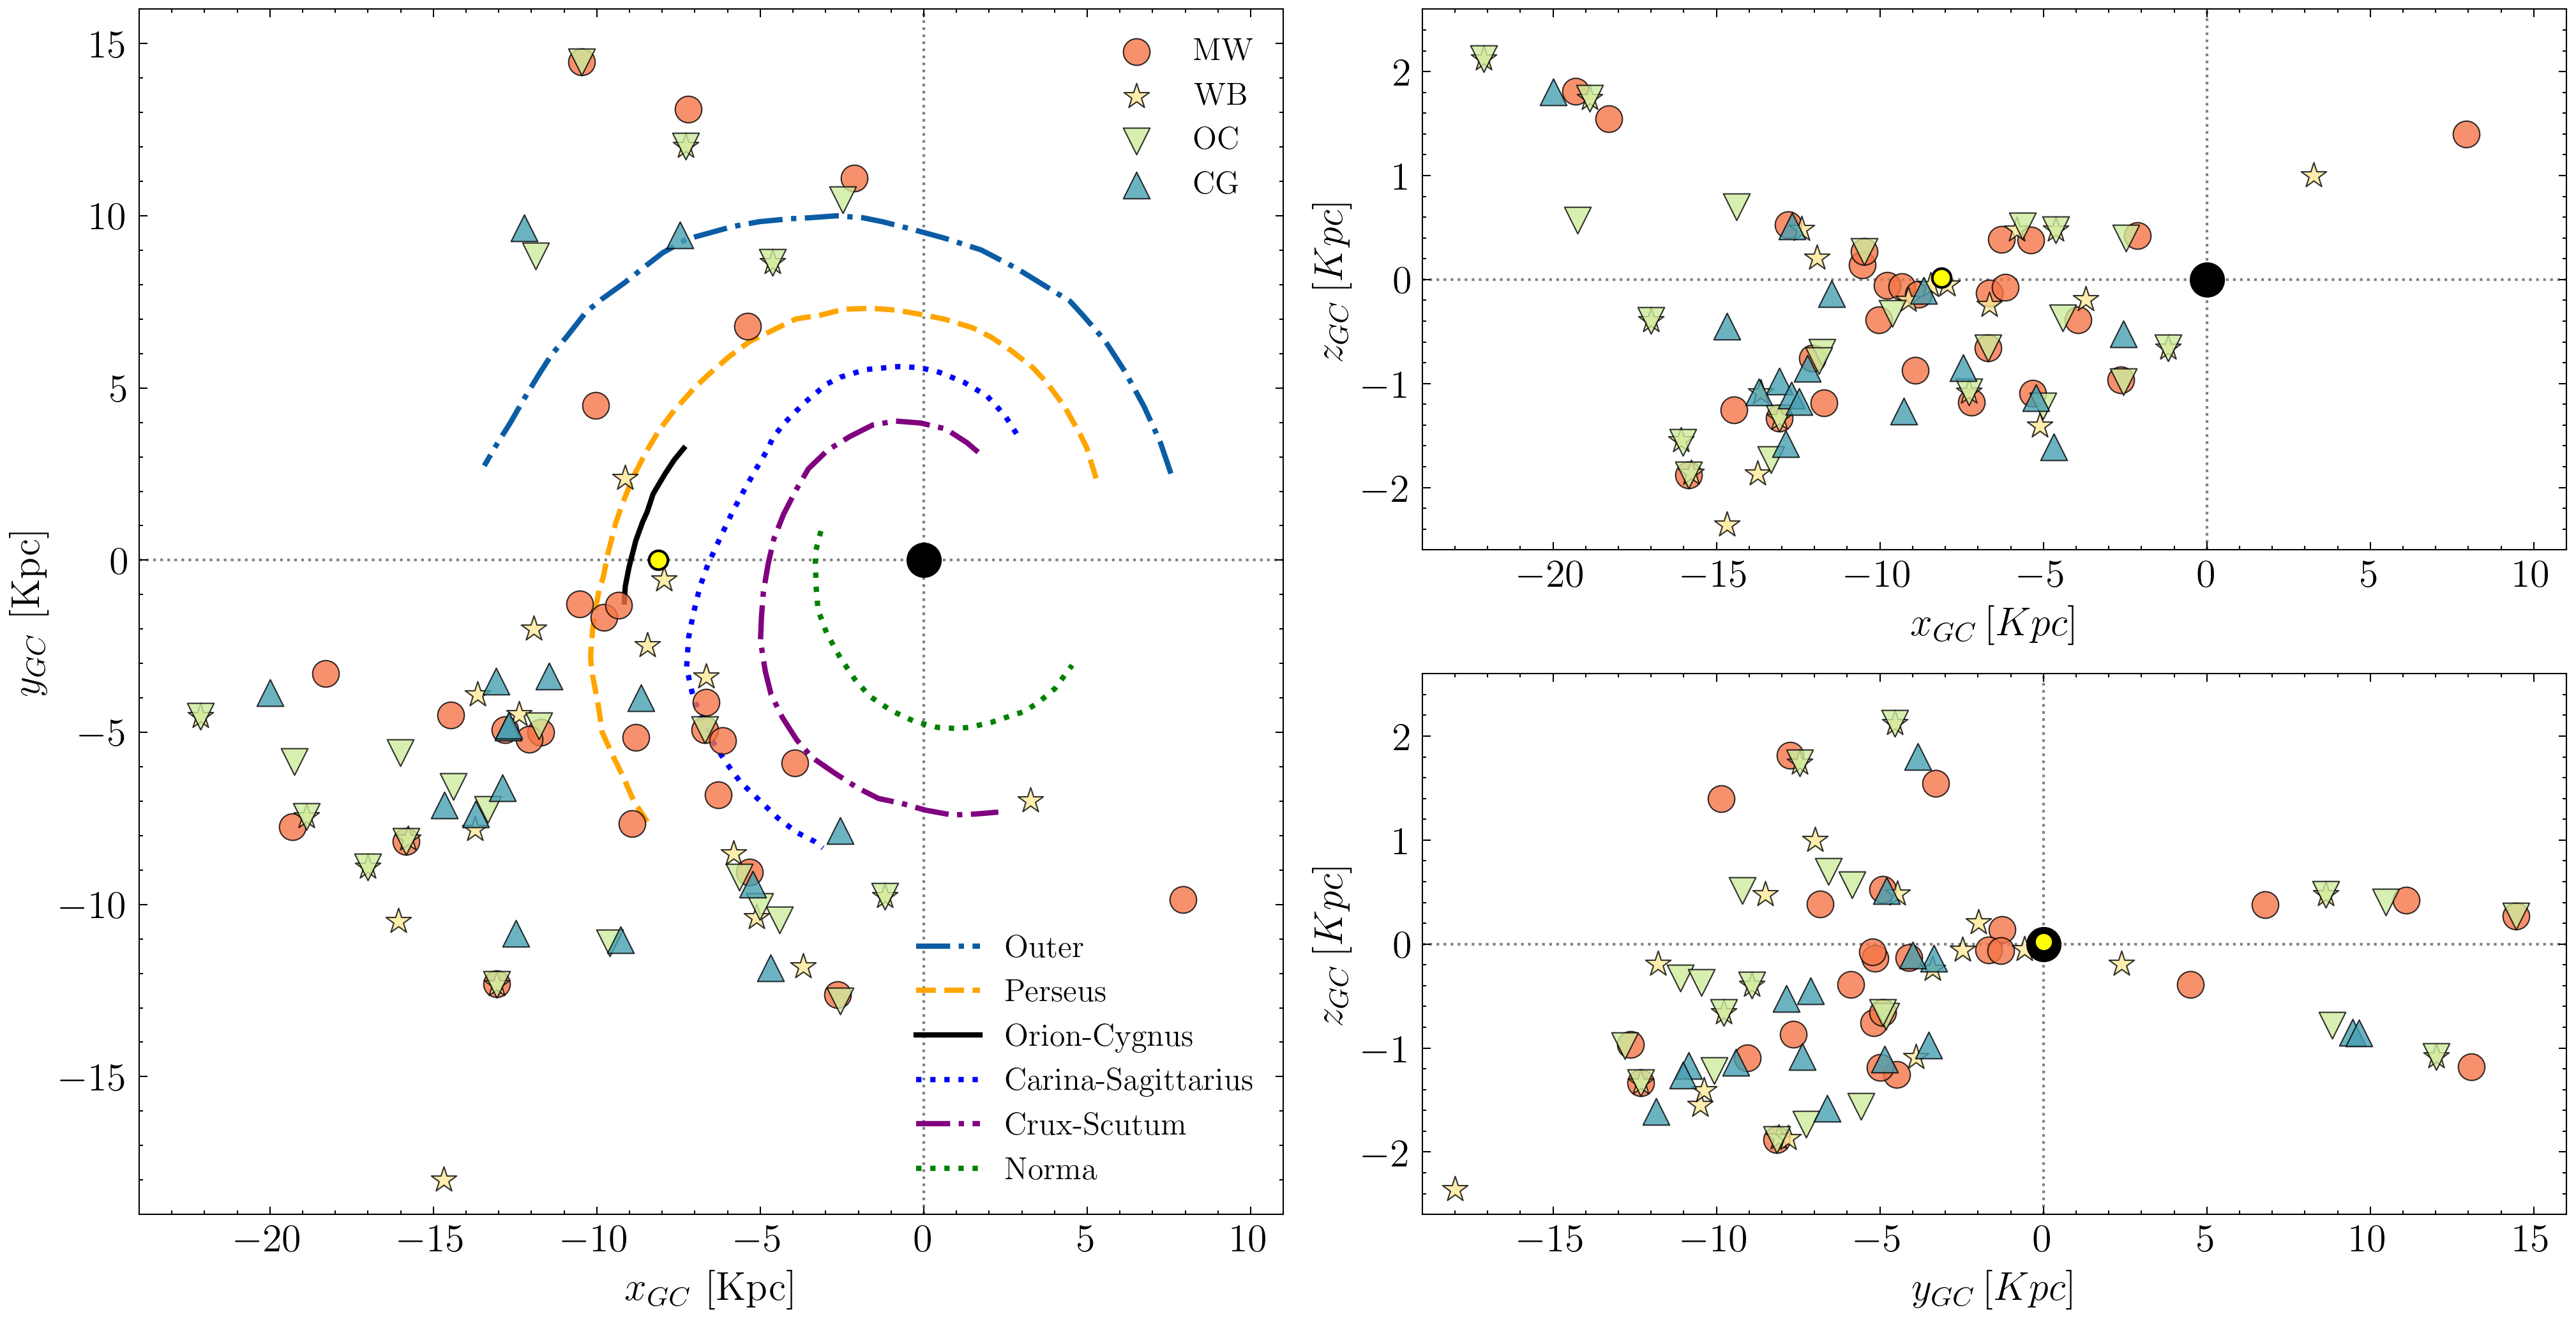
\includegraphics[]{figs/MWmap.png}}
  \caption{Right: position of the twenty-five clusters selected from the four
  catalogs mentioned in the text, on a face-on view of the Milky Way. The Sun
  and the center of the Galaxy are marked with a yellow filled circle and a
  black filled circle, respectively. Left, top and bottom: edge-on views,
  same color and marker conventions as above.}
  \label{fig:MWmap}
 \end{figure*}





% =============================================================================
\section{Cluster analysis}
 \label{sec:clust_analy}

 \subsection{Structural analysis}

  The first step in the cluster analysis is the estimation of their structural
  properties, i.e. center coordinates and limiting radius. Although centers and
  diameters are present in (some of) the catalogues, not all of these values are
  correct. We use our \texttt{ASteCA} package
  \citep{Perren_2015}\footnote{\url{http://asteca.github.io/}} throughout this
  work to perform the structural and fundamental parameters analysis. We have
  applied this tool to the study of hundreds of clusters in previous articles,
  with excellent results~\citep{Perren_2017,Perren_2020}.

  The center values are obtained applying a two-dimensional kernel density
  analysis (KDE) on each of the cluster's coordinates. This method assigns the
  center of the cluster to the point with the largest density in the frame. As
  shown in previous articles \citep{Perren_2015,Perren_2017,Perren_2020}, this
  approach is robust even when applied on frames with star densities that
  are very much non-uniform. See for example the case of van den Bergh-Hagen 37,
  shown in Fig.~\ref{fig:12struct}.

  A King's profile~\citep{King_1962} fit is performed on the radial
  density profile of each cluster to estimate their core and tidal radii
  ($r_{c}$, $r_{t}$). The adopted radius $r_{a}$ is the limiting distance from
  the center used to define the studied cluster region for each cluster. These
  radii are estimated applying a process that compares the ratio of the
  approximated number of true members for increasing radii values, with the
  number of stars in a concentric ring centered on each radius. The
  approximated number of members is obtained as the total number of stars within
  the radius, minus the expected number (field density times circle area). This
  method produces an overdensity around the value where the radial density
  approaches the field density, maximizing the contrast between members included
  within the radius and contaminating field stars. The method is also useful
  for heavily contaminated cluster, and/or clusters with very few true
  members. All radii values are shown in Table~\ref{tab:radii}.\\

  The adopted radius $r_{a}$ is on average 50\% smaller than the
  tidal radius (see Table~\ref{tab:radii}). This allows us to alleviate the
  issue of field star contamination, while ensuring that only a small number of
  true members (cluster stars located as far from the center as the tidal
  radius) are lost.
  The fraction of lost members can be estimated integrating King's profile. This
  fraction depends on the concentration of the cluster ($r_{t}/r_{c}$) and the
  value of the adopted radius as a fraction of the tidal radius ($r_{a}/r_{t}$).
  In our case, less than 20\% of the members could be lost in a worst case
  scenario. Since these are clusters that are strongly contaminated 
  (particularly in the parallax and proper motions spaces), the trade off
  between losing a small portion of members and improving the contrast of the
  true members over the field noise, is positive.

  The $r_{a}$ values used in our analysis being smaller than the tidal radius,
  means that the total estimated mass for each cluster shown in
  Sect.~\ref{sec:results} must be thought of as a lower limit.\\

  In Fig.~\ref{fig:BER29_struct} we show the structural analysis, center and
  radii estimation processes, for the cluster Berkeley 29. The asterisks in the
  equatorial coordinates of the left plot indicate that these were shifted
  and transformed so that the center of the frame is located at (0, 0) and to
  remove projection artifacts. The right plot shows the radial density analysis
  where the dashed green line and the shaded green area are the King profile fit
  and its 16th-84th uncertainty region, respectively. The green dotted vertical
  line, solid red vertical line, and solid green vertical line, are the core 
  ($r_{c}$), adopted ($r_{a}$), and tidal ($r_{t}$) radii, respectively. The
  dashed and dotted horizontal black lines are the field density estimate and
  its $\pm1\sigma$ region, respectively. The plots for the remaining cluster can
  be seen in Appendix~\ref{app:struct_analysis}.

  \begin{figure*}
   \resizebox{\hsize}{!}{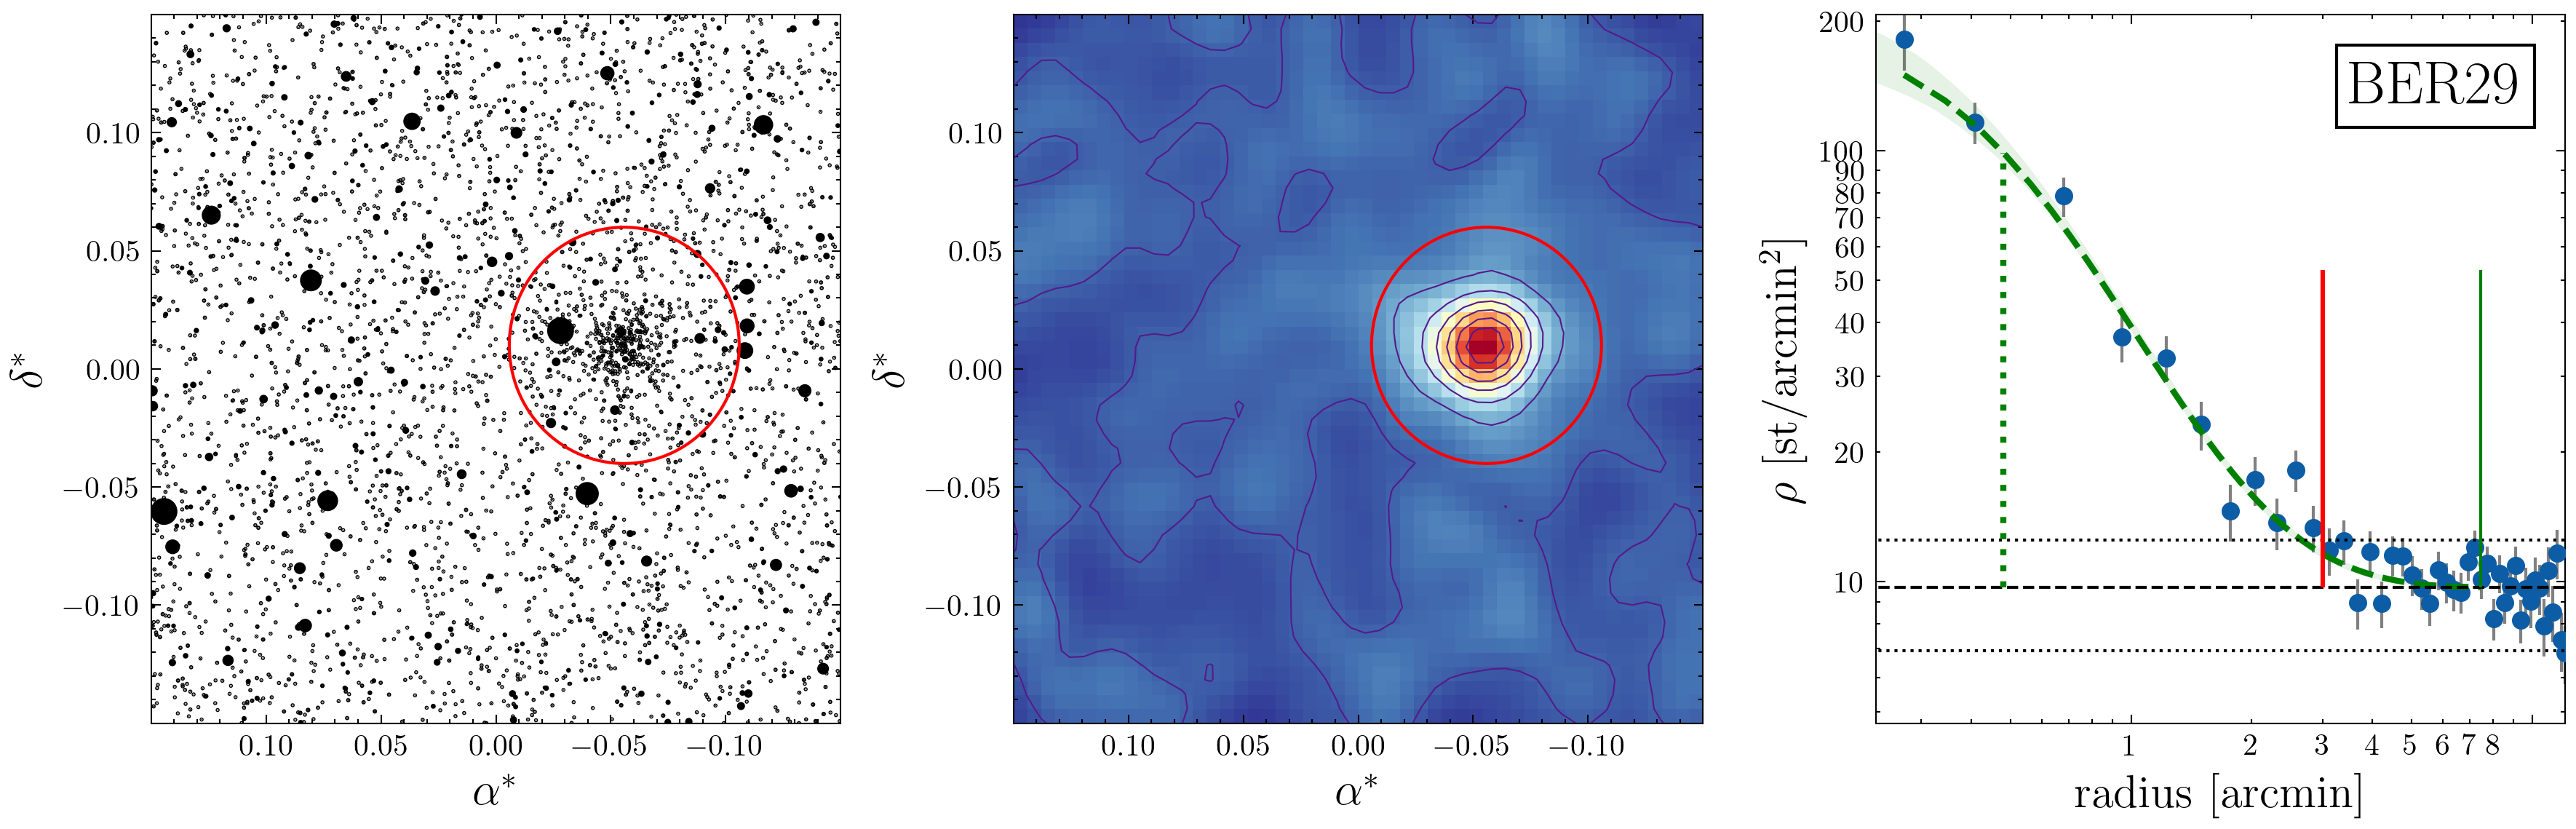
\includegraphics[]{figs/BER29_struct.png}}
   \caption{Left: analyzed $20^{\prime} \times 20^{\prime}$ arcmin frame with the
   estimated cluster region enclosed in a red circle. Center: same frame but
   shown as as two-dimensional density map. Right: radial density plot in
   logarithmic axis. Details in the body of the article.}
   \label{fig:BER29_struct}
  \end{figure*}




 \subsection{Membership and fundamental parameters}
  \label{ssec:fund_pars}

  \begin{figure*}
   \resizebox{\hsize}{!}{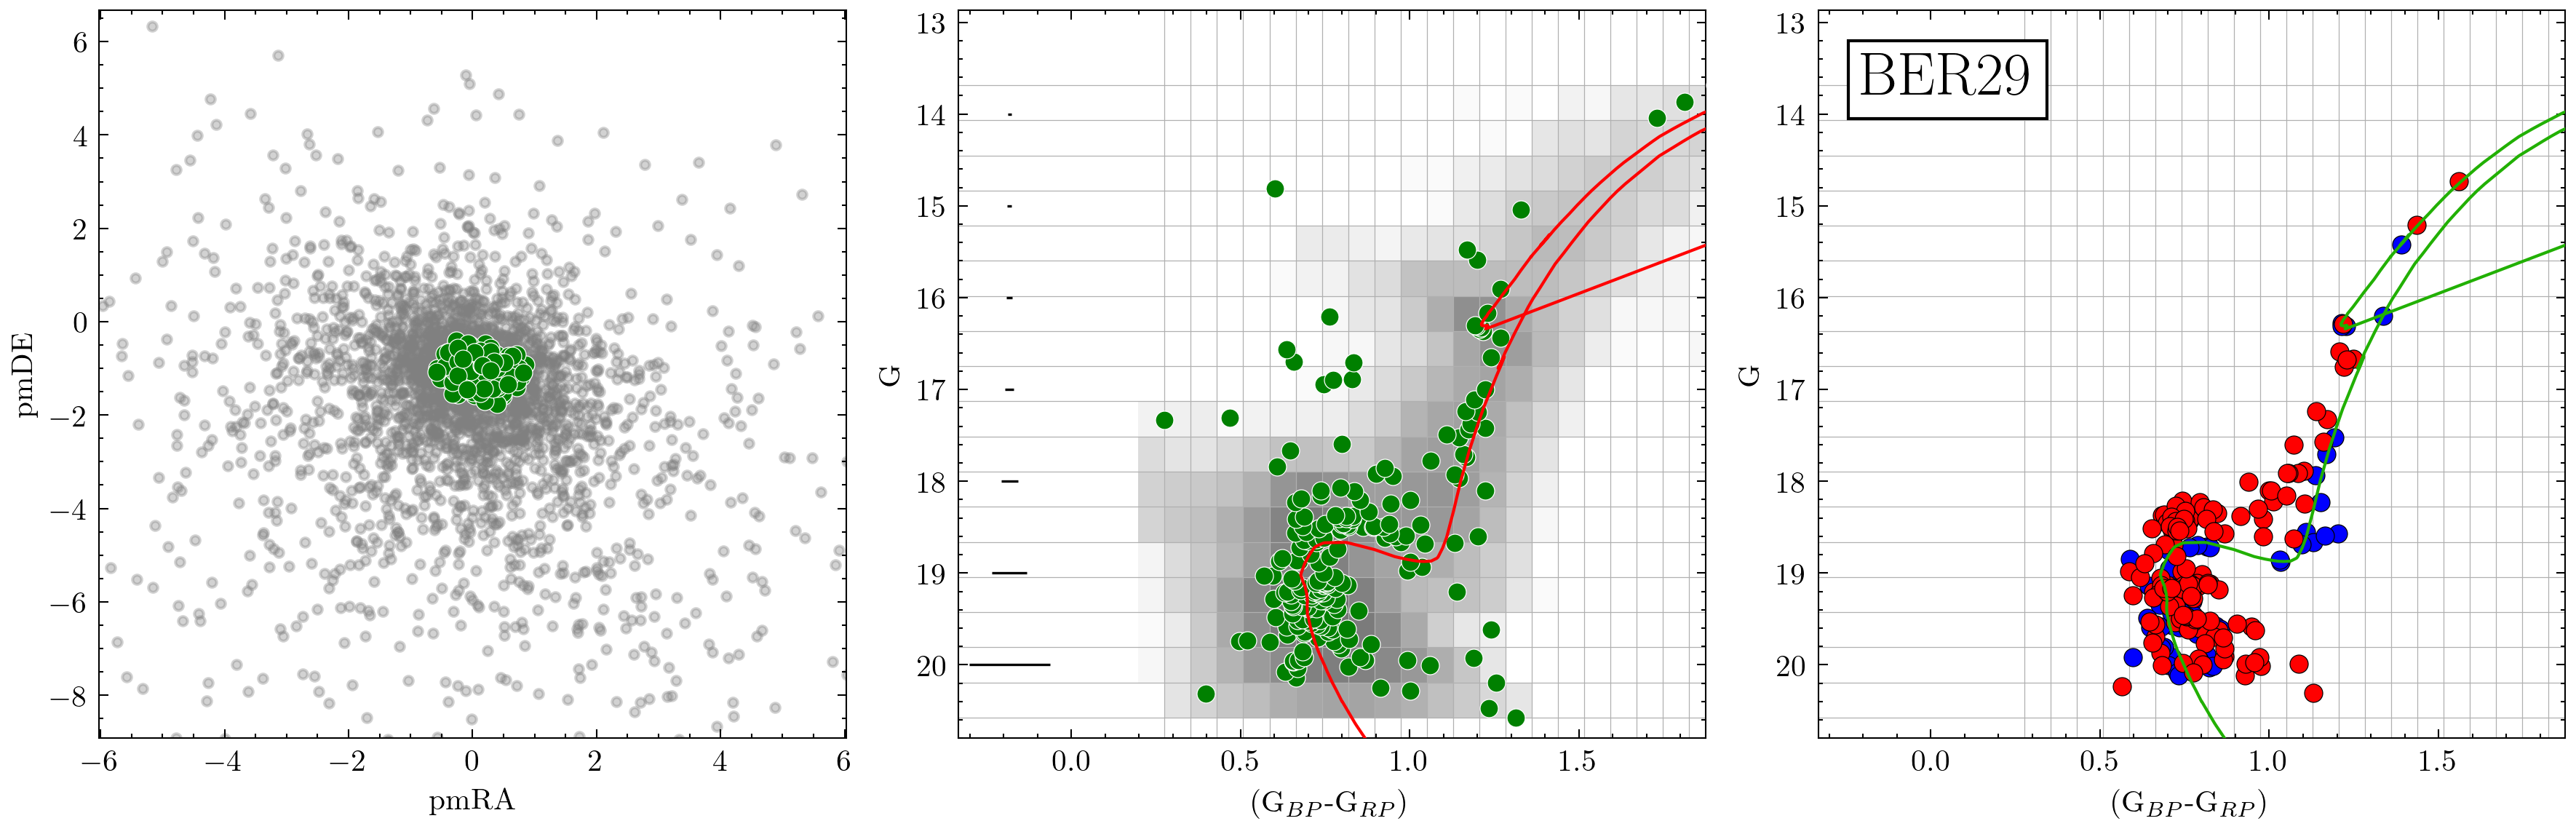
\includegraphics[]{figs/BER29_fpars.png}}
   \caption{Left: VPD for stars in the analyzed Berkeley 29
    frame; green and grey circles show the selected true members and the field
    stars, respectively.
    Center: CMD for the cluster's members with the isochrone associated to the
    best synthetic cluster fit drawn in red to guide the eye. The grey region
    represents the uncertainty in the fit.
    Right: best synthetic cluster fit found by \texttt{ASteCA} with the same
    isochrone now show in green. Blue and red circles are single and binary
    systems, respectively.}
   \label{fig:BER29_fpars}
  \end{figure*}

  Before we can estimate the fundamental parameters with \texttt{ASteCA}, we
  need to select the set of most probable members for each cluster. For this
  task we employed our recently developed pyUPMASK algorithm which demonstrated
  a great performance even for very contaminated clusters, outperforming
  UPMASK~\citep{Krone2014} as demonstrated in~\cite{Pera_2021}.

  pyUPMASk requires an input data set composed of $(\alpha, \delta)$ coordinates
  and at least two dimensions of data of any type to estimate the membership
  probabilities. We chose to make use of the proper motion data dimensions only,
  thus excluding photometric and parallax data.
  We made the decision of leaving out these extra data dimensions because,
  although they can be sometimes useful in the process of singling out the most
  probable members, for these type of very distant clusters they tend to add
  more noise than information.
  This is particularly true for the parallax data which
  rapidly tends to zero for stars beyond $\sim$2 kpc, where the parallax values
  for the cluster members become almost indistinguishable from the contaminating
  field stars. The selected clustering method in pyPMASK was a Gaussian Mixture
  Model, which demonstrated to have the best performance in~\cite{Pera_2021} 
  (see Sect. 4).

  Once pyUPMASK has assigned membership probabilities to all the stars in the
  frame, we must select the set of stars that most likely belong to the
  cluster (i.e., the true members). This step is usually handled by selecting
  an arbitrary cut-off probability value; in~\cite{Cantat_2020} for example
  the authors fix this value to P=70\%. Instead of setting an ad-hoc value, we
  performed an analysis that combines the membership probabilities with the
  stellar density inside and outside of the cluster region. This allows us to
  estimate the number of cluster members expected within the cluster region.
  Combining this number with the membership probabilities given by pyUPMASK we
  select those stars with the largest probabilities within the cluster region,
  such that the resulting total number of members is as close as possible as the
  expected one (i.e., the one obtained through the stellar density analysis).
  Using a physically reasonable number of members not only reduces the
  probability of excluding true members (by only selecting those with the
  largest membership probabilities), it also ensures that the estimation of the
  total mass parameter is properly performed by \texttt{ASteCA}.\\

  After selecting the set of true members for all the clusters as described
  above, we apply our \texttt{ASteCA} package to estimate the fundamental
  parameters: metallicity, age, total mass, fraction of binary systems,
  distance, and extinction. The code uses the ptemcee parallel tempering
  Bayesian inference algorithm~\citep{ptemcee} to sample the fundamental
  parameters' distributions. The likelihood function employed to asses the fit
  between the observed cluster and the synthetic clusters is the Bayesian
  Poisson ratio defined in~\cite{Tremmel_2013}.
  The theoretical isochrones used to generate the
  synthetic clusters used to match the observed clusters are the PARSEC
  tracks~\citep{Bressan_2012}. Priors are uniform for all the parameters using
  the following limiting ranges:

  \begin{itemize}
   \item metallicity (z): [0.001, 0.03]
   \item logarithmic age: [8, 10.1]
   \item total mass: [1e2, 2e5] $M_{\odot}$
   \item binarity fraction: [0, 1]
   \item distance modulus: [10, 20] mag
   \item $E_{BV}$ extinction: [0, $E_{BV}^{max}$]
  \end{itemize}

  \noindent The maximum value for the extinction priors, $E_{BV}^{max}$, was set
  on a per-cluster basis selecting the values given by the~\cite{Schlegel_1998}
  extinction maps with the re-calibration by~\cite{Schlafly_2011}.
  
  In Fig.~\ref{fig:BER29_fpars} we show the result of the membership
  probabilities estimation done with pyUPMASK, plus the fundamental parameters
  estimation performed by \texttt{ASteCA}. We only show here the plots for
  the cluster Berkeley 29, the remaining clusters can be seen in
  Appendix~\ref{app:fundam_params}.
  The plot on the left shows the vector point diagram (VPD) with the proper
  motion distributions for both the selected clusters members, and the field
  stars. The members are clearly very much embedded within the field stars
  distribution, which is expected for distant clusters. The center plot shows
  the CMD traced by the selected members, and the right plot a sampling of the
  best fit synthetic cluster obtained. The isochrone is associated with the
  synthetic cluster but it is there merely to guide the eye, the fit is
  performed for the CMD of the observed cluster versus the CMD of synthetic
  clusters, not versus theoretical isochrones~\citep[this is further
  explained in:][]{Perren_2015,Perren_2017,Perren_2020}.\\








% =============================================================================
\section{Results and discussion}
 \label{sec:results}

 This section is divided as follows.
 In Sect.~\ref{ssec:databases} we show the general results for the
 fundamental parameters. These are contrasted with values taken from the
 aforementioned databases, with particular emphasis on the distances.
 %
 Following that, in Sect.~\ref{ssec:indiv_clusters} we discuss each cluster
 individually. We comment on the most relevant studies published in the
 literature and how these compare to the results obtained in this article.
 %
 Finally, in Sect.~\ref{ssec:met_gradient} we analyze our results in the context
 of the radial metallicity gradient and the age vs metallicity relation.\\

 Henceforth we employ the default values for the Galactocentric coordinate
 frame given by the astropy
 package\footnote{\url{https://docs.astropy.org/en/stable/coordinates/galactocentric.html}}:

 \begin{itemize}
  \item ICRS coordinates of the Galactic center: (266.4051$^{\circ}$,\\
  -28.936175$^{\circ}$)
  \item Distance from the sun to the Galactic center: 8.122 pc
  \item Distance from the sun to the Galactic midplane: 20.8 pc
  \item Velocity of the sun in the Galactocentric frame as Cartesian velocity
  components: (12.9, 245.6, 7.78) km/s
 \end{itemize}




  \subsection{Comparision with databases}
  \label{ssec:databases}

  \begin{table*}
  \caption{Fundamental parameters estimated with \texttt{ASteCA} for the
  twenty-five analyzed clusters. Sub and supra indexes indicate the 16th
  and 84th percentiles, respectively. The last column indicates the number of
  true members used in the analysis.}
  \label{tab:results}
  \centering
  \begin{tabular}{lccccccc}
  \hline\hline
  Cluster & $z$ & $\log{age}$ & $E_{BV}$ & dm$_{\odot}$ & M (M$_{\odot}$) & b$_
  {fr}$ & N\\
  \hline %\\[.2cm]
  BER73 & 0.0051$_{0.0009}^{0.0153}$ & 9.76$_{9.30}^{9.93}$ & 0.23$_{0.10}^{0.32}$ &
  13.45$_{13.16}^{14.13}$ & 2.7E+03$_{1.9E+03}^{4.8E+03}$ & 0.44$_{0.21}^{0.75}$
  & 105\\[.2cm]
  BER25 &  0.0157$_{0.0079}^{0.0173}$ & 9.78$_{9.69}^{9.81}$ & 0.34$_{0.32}^{0.41}$ &
  14.29$_{14.12}^{14.39}$ & 1.4E+04$_{9.0E+03}^{2.3E+04}$ & 0.76$_{0.51}^{0.93}$
  & 220 \\[.2cm]
  BER75 & 0.0084$_{0.0019}^{0.0187}$ & 9.78 $_{9.59}^{9.93 }$ & 0.10$_{0.03}^{0.15}$ &
  14.50$_{14.16}^{14.82}$ & 7.0E+03$_{2.9E+03}^{1.3E+04}$ & 0.79$_{0.21}^{0.96}$ &
  99 \\[.2cm]
  BER26 & 0.0215$_{0.0125}^{0.0277}$ & 9.91 $_{9.72}^{10.05}$ & 0.55$_{0.50}^{0.58}$ &
  13.38$_{12.98}^{13.81}$ & 4.7E+03$_{2.3E+03}^{8.1E+03}$ & 0.76$_{0.46}^{0.94}$ &
  79 \\[.2cm]
  BER29 & 0.0108$_{0.0051}^{0.0174}$ & 9.60 $_{9.55}^{9.65 }$ & 0.05$_{0.01}^{0.11}$ &
  15.76$_{15.64}^{15.88}$ & 1.1E+04$_{7.3E+03}^{2.0E+04}$ & 0.60$_{0.34}^{0.83}$ &
  218 \\[.2cm]
  TOMB2 & 0.0068$_{0.0057}^{0.0070}$ & 9.30 $_{9.29}^{9.31 }$ & 0.38$_{0.38}^{0.41}$ &
  14.75$_{14.72}^{14.76}$ & 1.7E+04$_{1.6E+04}^{1.9E+04}$ & 0.38$_{0.34}^{0.43}$ &
  907 \\[.2cm]
  BER76 & 0.0155$_{0.0099}^{0.0208}$ & 9.25 $_{9.22}^{9.30 }$ & 0.58$_{0.54}^{0.63}$ &
  13.70$_{13.56}^{13.85}$ & 4.6E+03$_{2.9E+03}^{6.7E+03}$ & 0.65$_{0.44}^{0.80}$ &
  160 \\[.2cm]
  F1212 & 0.0162$_{0.0088}^{0.0250}$ & 9.08 $_{9.01}^{9.14 }$ & 0.65$_{0.59}^{0.71}$ &
  15.03$_{14.85}^{15.32}$ & 4.6E+03$_{3.3E+03}^{8.3E+03}$ & 0.47$_{0.30}^{0.76}$ &
  100 \\[.2cm]
  SAU1  & 0.0211$_{0.0125}^{0.0261}$ & 9.81 $_{9.66}^{9.95 }$ & 0.09$_{0.05}^{0.15}$ &
  15.48$_{15.23}^{15.75}$ & 9.7E+03$_{4.7E+03}^{1.7E+04}$ & 0.81$_{0.48}^{0.95}$ &
  90 \\[.2cm]
  CZER30 & 0.0100$_{0.0044}^{0.0216}$ & 9.54 $_{9.44}^{9.67 }$ & 0.27$_{0.18}^{0.36}$ &
  14.09$_{13.93}^{14.22}$ & 7.2E+03$_{4.4E+03}^{1.2E+04}$ & 0.78$_{0.56}^{0.93}$ &
  120 \\[.2cm]
  ARPM2 & 0.0087$_{0.0039}^{0.0120}$ & 9.59 $_{9.53}^{9.68 }$ & 0.62$_{0.59}^{0.68}$ &
  15.20$_{15.11}^{15.31}$ & 8.8E+03$_{6.7E+03}^{1.3E+04}$ & 0.30$_{0.16}^{0.54}$ &
  200 \\[.2cm]
  BH4 & 0.0079$_{0.0017}^{0.0245}$ & 9.14 $_{8.75}^{9.42 }$ & 0.42$_{0.08}^{0.48}$ &
  14.48$_{13.90}^{15.32}$ & 1.9E+03$_{1.0E+03}^{3.5E+03}$ & 0.62$_{0.29}^{0.86}$ &
  70 \\[.2cm]
  F1419 & 0.0243$_{0.0123}^{0.0279}$ & 9.60 $_{9.52}^{9.78 }$ & 0.52$_{0.49}^{0.59}$ &
  14.85$_{14.57}^{15.00}$ & 9.4E+03$_{6.4E+03}^{1.7E+04}$ & 0.56$_{0.30}^{0.85}$ &
  150 \\[.2cm]
  BH37 & 0.0163$_{0.0043}^{0.0241}$ & 8.90 $_{8.61}^{9.68 }$ & 1.21$_{0.80}^{1.34}$ &
  12.22$_{10.97}^{12.86}$ & 2.4E+03$_{1.4E+03}^{4.1E+03}$ & 0.51$_{0.29}^{0.79}$ &
  90 \\[.2cm]
  E9205 & 0.0202$_{0.0124}^{0.0210}$ & 9.74 $_{9.72}^{9.78 }$ & 0.06$_{0.05}^{0.12}$ &
  15.57$_{15.52}^{15.62}$ & 3.3E+04$_{2.4E+04}^{4.1E+04}$ & 0.72$_{0.61}^{0.82}$ &
  400 \\[.2cm]
  E9218 & 0.0178$_{0.0125}^{0.0184}$ & 9.74 $_{9.73}^{9.78 }$ & 0.16$_{0.15}^{0.19}$ &
  15.24$_{15.21}^{15.29}$ & 4.5E+04$_{4.0E+04}^{5.4E+04}$ & 0.57$_{0.47}^{0.67}$ &
  823 \\[.2cm]
  SAU3 & 0.0207$_{0.0078}^{0.0277}$ & 9.64 $_{9.53}^{9.88 }$ & 0.69$_{0.66}^{0.76}$ &
  14.10$_{13.82}^{14.49}$ & 1.5E+04$_{7.8E+03}^{2.1E+04}$ & 0.89$_{0.61}^{0.96}$ &
  160 \\[.2cm]
  KRON39 & 0.0151$_{0.0074}^{0.0251}$ & 9.46 $_{9.34}^{9.69 }$ & 0.75$_{0.67}^{0.84}$ &
  15.54$_{15.20}^{15.80}$ & 1.2E+04$_{5.9E+03}^{2.5E+04}$ & 0.72$_{0.36}^{0.93}$ &
  80 \\[.2cm]
  E9308 & 0.0073$_{0.0023}^{0.0182}$ & 9.93 $_{9.54}^{10.05}$ & 0.67$_{0.58}^{0.79}$ &
  15.61$_{15.37}^{15.83}$ & 3.4E+04$_{1.5E+04}^{6.7E+04}$ & 0.66$_{0.31}^{0.89}$ &
  65 \\[.2cm]
  BH144 & 0.0034$_{0.0031}^{0.0057}$ & 9.02 $_{8.93}^{9.10 }$ & 0.82$_{0.78}^{0.88}$ &
  14.90$_{14.83}^{15.06}$ & 6.6E+03$_{5.7E+03}^{8.0E+03}$ & 0.36$_{0.27}^{0.45}$ &
  400 \\[.2cm]
  % BH176 & 0.0116$_{0.0054}^{0.0177}$ & 10.03$_{9.81}^{10.06}$ & 0.58$_{0.51}^{0.64}$ &
  % 15.93$_{15.88}^{15.98}$ & 1.7E+05$_{1.4E+05}^{1.9E+05}$ & 0.39$_{0.17}^{0.54}$\\[.2cm]
  BH176 & 0.0256$_{0.0122}^{0.0272}$ & 9.71$_{9.68}^{9.77}$ & 0.44$_{0.42}^{0.50}$ &
  16.48$_{16.42}^{16.53}$ & 1.7E+05$_{1.4E+05}^{1.9E+05}$ & 0.46$_{0.29}^{0.60}$ &
  333 \\[.2cm]
  KRON31 & 0.0155$_{0.0068}^{0.0243}$ & 8.99 $_{8.91}^{9.07 }$ & 1.24$_{1.18}^{1.32}$ &
  14.59$_{14.31}^{14.80}$ & 8.2E+03$_{5.5E+03}^{1.3E+04}$ & 0.78$_{0.61}^{0.92}$ &
  150 \\[.2cm]
  SAU6 & 0.0149$_{0.0065}^{0.0248}$ & 9.15 $_{9.05}^{9.53 }$ & 0.92$_{0.81}^{1.03}$ &
  14.85$_{14.11}^{15.15}$ & 4.9E+03$_{3.3E+03}^{7.5E+03}$ & 0.52$_{0.33}^{0.72}$ &
  153 \\[.2cm]
  BER56 & 0.0181$_{0.0065}^{0.0265}$ & 9.75 $_{9.72}^{9.76 }$ & 0.42$_{0.38}^{0.51}$ &
  15.21$_{15.16}^{15.25}$ & 5.9E+04$_{4.8E+04}^{7.1E+04}$ & 0.66$_{0.57}^{0.74}$ &
  900 \\[.2cm]
  BER102 & 0.0111$_{0.0059}^{0.0228}$ & 9.69 $_{9.57}^{9.82 }$ & 0.44$_{0.37}^{0.51}$ &
  14.43$_{14.19}^{14.61}$ & 6.2E+03$_{4.1E+03}^{9.4E+03}$ & 0.59$_{0.38}^{0.78}$ &
  160 \\[.2cm]
  \hline
  \end{tabular}
  \end{table*}

  Table~\ref{tab:results} shows the fundamental parameters along with their
  uncertainties estimated by \texttt{ASteCA}. The Bayesian inference process was
  allowed to run for enough steps to achieve convergence.
  As shown in the table all the analyzed clusters are rather old, with the
  youngest one (vd Bergh-Hagen 37) assigned an age of $\sim1$ Gyr; although
  notice the very large uncertainty associated to it. It is worth noting
  that only about half of the clusters are truly beyond the 9 kpc ($\sim$14.8
  mag) limit originally used to perform the selection from the published
  databases.\\

  In a recent study~\citep{Anders_2021} per-star parameters such as distance,
  extinction, metallicity, and age were estimated. Comparing the results
  from this analysis with those from \cite{Cantat_2020}, the authors find
  differences in the distance values larger than 3 kpc for clusters located at
  6 kpc or more from the Sun. We find even larger discrepancies between our
  analysis and those taken from the four databases. As shown in
  Fig.~\ref{fig:distances}, all but the CG20 database show differences of up
  to 10 kpc for clusters spanning the full distance range. Even the CG20
  database, the one with the better overall match to our values, shows
  differences more than 2 kpc for clusters located at a distance of $\sim10$ kpc
  from the Sun. It is thus clear that even the database with the closest fit
  contains substantial disagreements with the distance values estimated by 
  \texttt{ASteCA}. We see no evident trend that correlates the differences in
  the distance with the ages (used to color the circles in
  Fig.~\ref{fig:distances}).\\


  \begin{figure*}
   \resizebox{\hsize}{!}{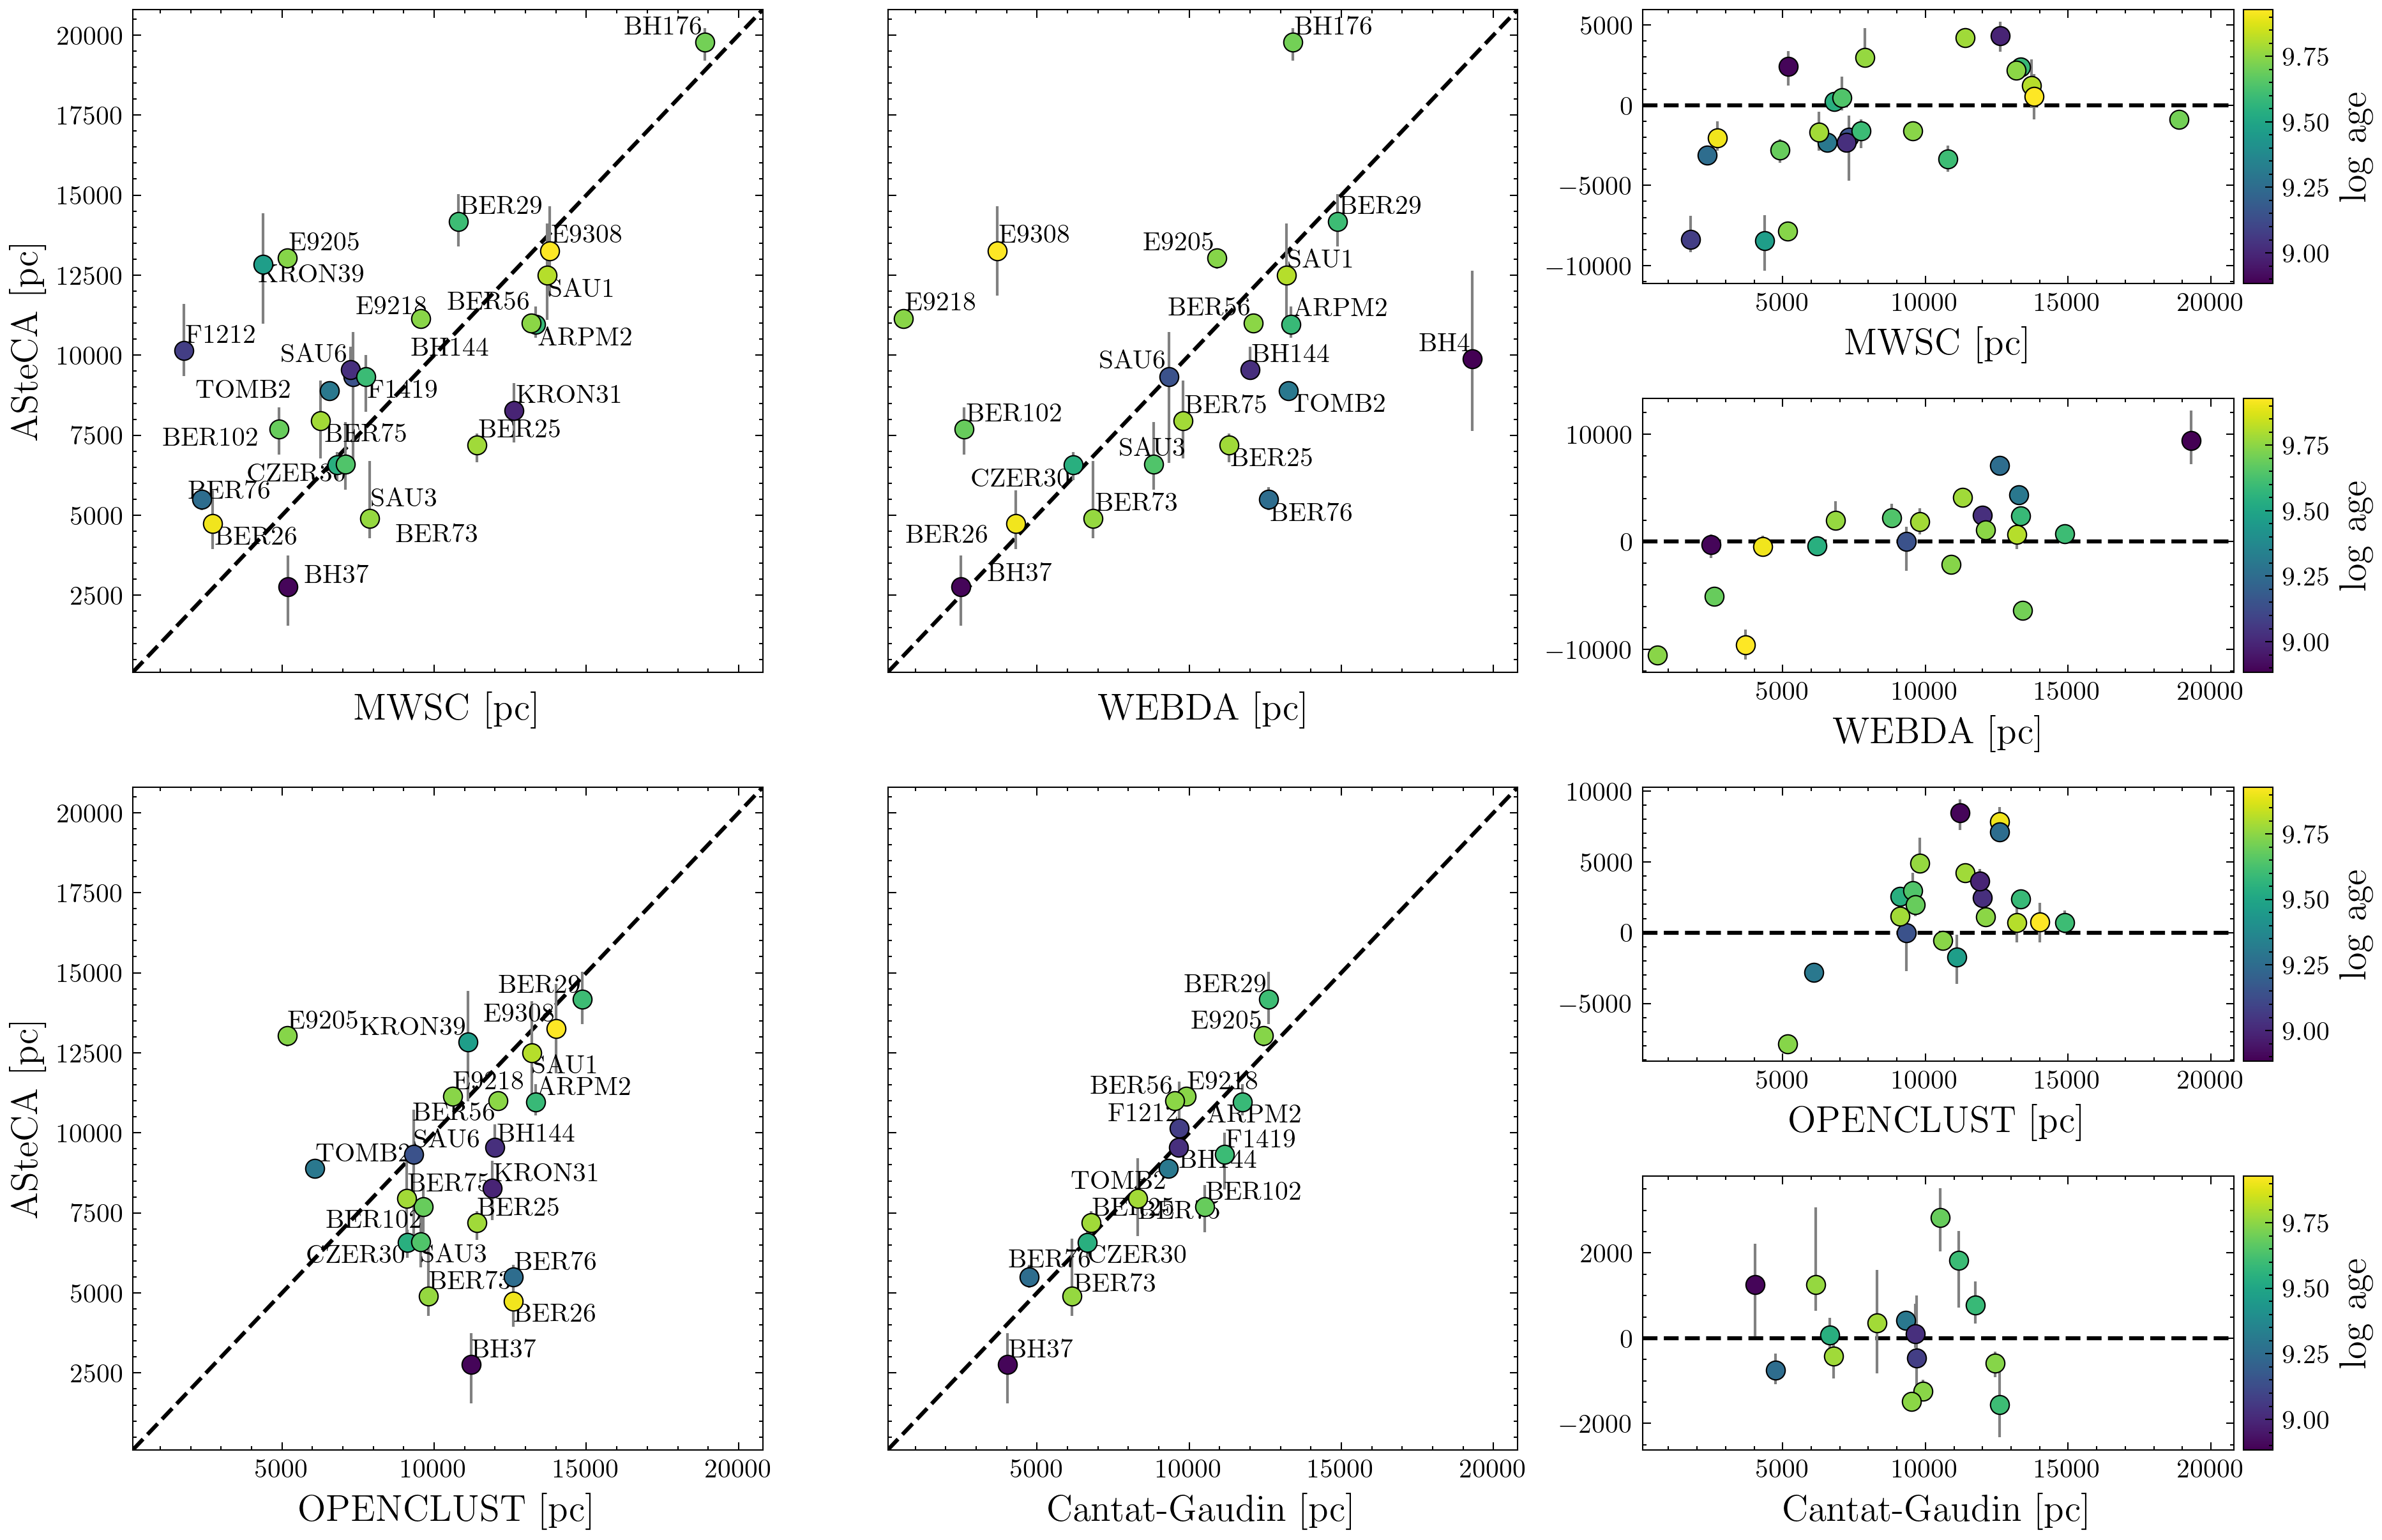
\includegraphics[]{figs/dist.png}}
   \caption{\texttt{ASteCA} versus database distances. The plots to the right
   stacked vertically are the \texttt{ASteCA} distances versus the differences
   in the sense (\texttt{ASteCA} - database). Clusters are colored according to
   the $\log\,age$} assigned by \texttt{ASteCA}.
   \label{fig:distances}
  \end{figure*}

  We can analyze the difference between our age estimation and those from
  the four databases; the results are shown in Fig.~\ref{fig:ages}. The plot
  shows that \texttt{ASteCA} assigns ages that are larger on average than the
  databases, and more so as the estimated age increases. A difference of 3 Gyr
  for an age of 8 Gyr (the average difference shown in the plot) translates to a
  logarithmic difference of $\sim$ 0.2 dex, which is a reasonable uncertainty
  given the complexities associated to the clusters under investigation. The
  largest difference arises with Kronberger 39, for which \texttt{ASteCA} finds
  an age of $\log(age)=9.5$ but has an age of $\log(age)=6$ assigned in the
  MWSC database (the smallest age by far in the four databases).\\

  \begin{figure}
   \resizebox{\hsize}{!}{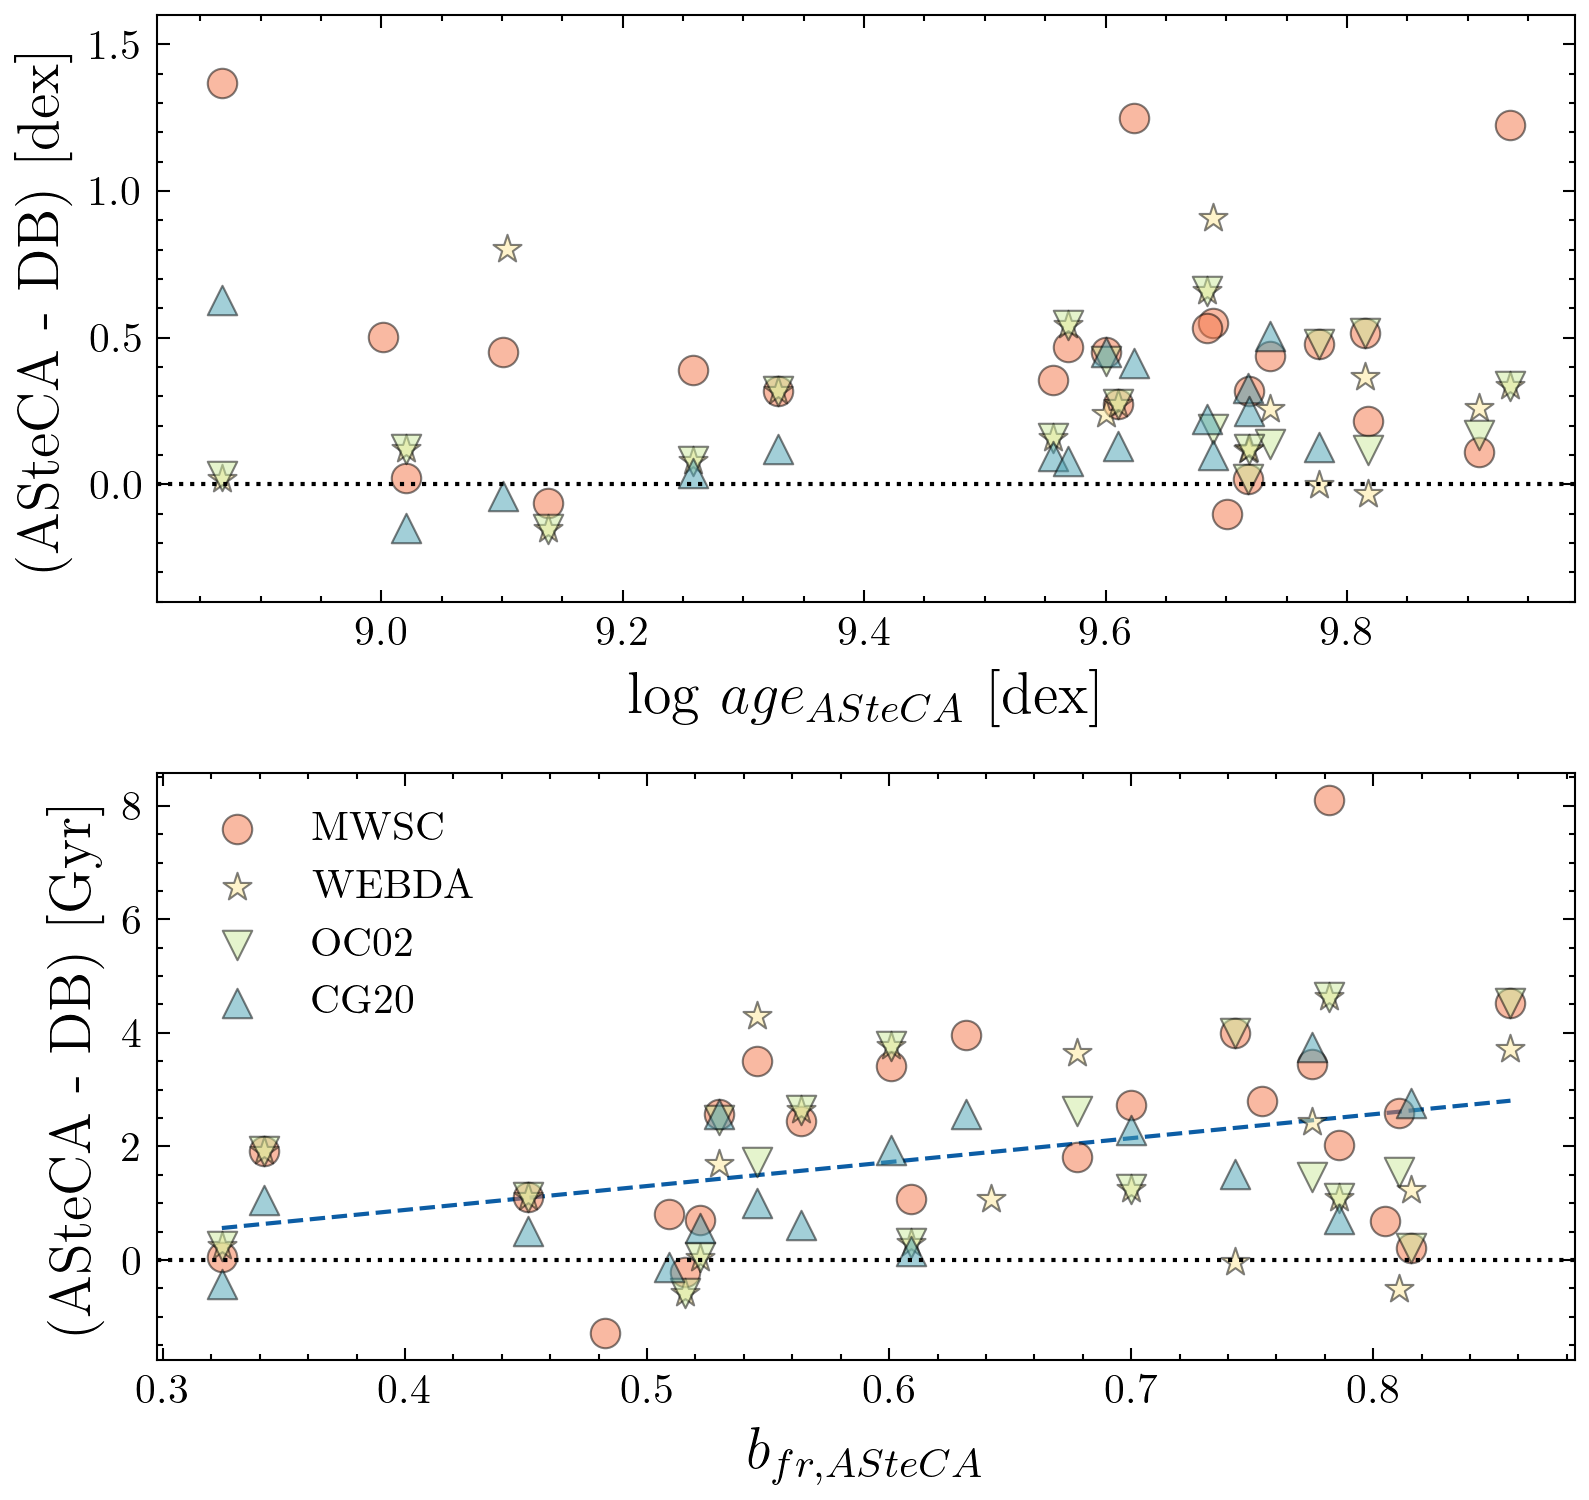
\includegraphics[]{figs/ages.png}}
   \caption{\texttt{ASteCA} ages versus difference between databases age
   estimates in the sense (\texttt{ASteCA} - database).}
   \label{fig:ages}
  \end{figure}


  To further investigate the various ways to estimate the distance, we performed
  two more analyses. First, we re-run \texttt{ASteCA} for all the
  clusters using four different combinations of settings for the metallicity and
  binary fraction parameters. We chose these two parameters because in
  isochrone-fit analyses they are usually either fixed (e.g., the metallicity is
  set to solar) or neglected altogether (e.g., the binary fraction).
  %
  Second, we compared the distances estimated in this work with those obtained
  via parallax analysis using three different methods: \texttt{ASteCA}'s own
  Bayesian inference estimation~\citep[described in][]{Perren_2020}, the
  distance inferred by the Kalkayotl package~\citep{Kalkayotl}, and the median
  of a simple inversion of the parallax values of the selected members.
  Parallax values were previously corrected using the method described
  in~\cite{Lindegren_2021}\footnote{ Analytical functions to compute the
  expected parallax zero-point as a function of ecliptic latitude, magnitude and
  colour for any Gaia (e)DR3
  source: \url{https://gitlab.com/icc-ub/public/gaiadr3_zeropoint}}.\\

  The results of the two extra analysis mentioned above can be seen in
  Fig.~\ref{fig:dist_comparisions} compared to the main \texttt{ASteCA} run,
  i.e., the one whose estimated parameter values are shown in
  Table~\ref{tab:results}.
  In the top plot we show the variation in the distance estimates between our
  main \texttt{ASteCA} run and four different runs: metallicity fixed to solar
  and binary fraction fixed to 0 ($Z=Z_{\odot},b_{fr}=0.0$; blue circles),
  metallicity fixed to solar and binary fraction as a free parameter
  ($Z=Z_{\odot}$; green stars), metallicity as a free parameter and binary
  fraction fixed to 0 ($b_{fr}=0.0$; orange triangles), and metallicity fixed to
  solar and binary fraction fixed to 0.3 ($Z=Z_{\odot},b_{fr}=0.3$; red
  inverted triangles), where 0.3 is usually chosen to be a reasonable estimate
  for open clusters~\citep{Sollima_2010}. The median difference with the main
  \texttt{ASteCA} run is largest when the binary fraction is fixed to 0. 
  ($\sim$1100 pc), lower when we fix this parameter to 0.3 ($\sim$500 pc),
  and lowest when it is allowed to vary ($\sim$25 pc). This indicates that a
  proper binary fraction fit is of utmost importance for a correct estimation of
  the cluster's fundamental parameters, particularly for the distance. Even when
  the binary fraction is free, fixing just the metallicity to solar values can
  have a large impact on the estimated distances as shown in
  Fig.~\ref{fig:dist_comparisions} (green stars).
  % $Z=Z_{\odot},b_{fr}=0.0$: 1157
  % $Z=Z_{\odot}$: -25
  % $b_{fr}=0.0$: 1182
  % $Z=Z_{\odot},b_{fr}=0.3$: 518


  The bottom plot in Fig.~\ref{fig:dist_comparisions} shows the parallax values
  analysis. Here the distance estimates obtained by \texttt{ASteCA} processing
  the Gaia eDR3 photometry are compared to three methods to estimate distances
  using parallaxes: \texttt{ASteCA}'s own Bayesian inference, the Kalkayotl
  package estimate, and the inversion of the median of the selected member's
  parallaxes. It is clear to see that a trend arises where the most distant
  clusters have their distances enormously underestimated by any of the
  parallax-based methods. This is expected, as the parallax values of the most
  distant clusters are associated to very large uncertainties and are also
  heavily affected by noise from non-removed field stars that mostly contaminate
  the lower mass region.
  It is surprising to see that the naive approach of inverting the median of
  the member's parallaxes is the method that more closely approximates the
  photometric distances estimated by \texttt{ASteCA}: the mean difference is
  only $\sim$ 600 pc, where the other two methods show median differences more
  that twice as large ($\sim$ 1300 pc).
  % median(Plx)$^{-1}$: 617
  % ASteCA: 1396
  % Kalkayotl: 1308
  \\


  \begin{figure}
   \resizebox{\hsize}{!}{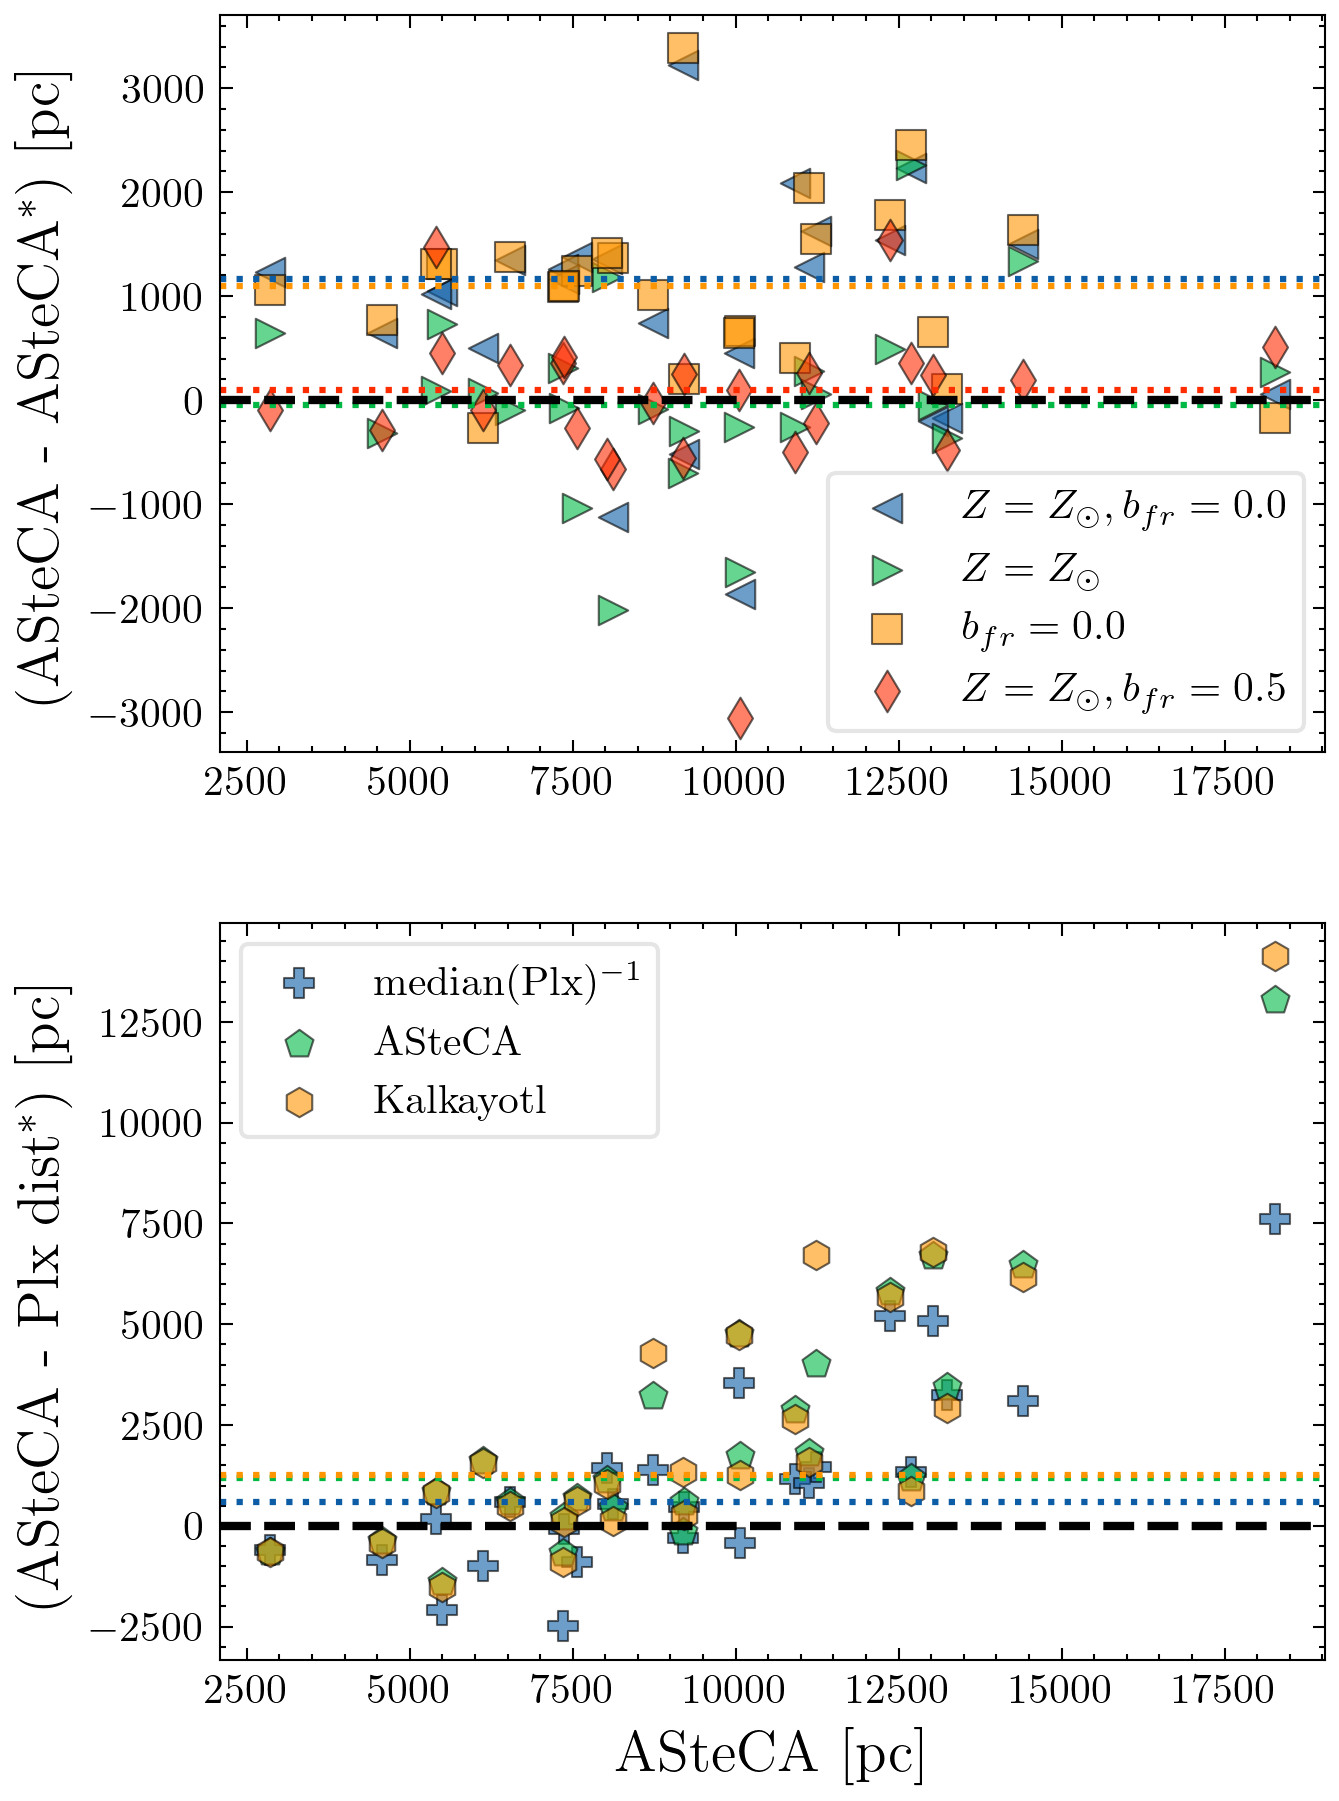
\includegraphics[]{figs/d_zb_fixed_plx.png}}
   \caption{Top: distances estimated with the main run of \texttt{ASteCA}
   compared to four different runs where the metallicity and binary fraction
   were wither fixed or allowed to be fitted.
   Bottom: main run distances versus the difference with the distances
   estimated using parallax values and three different methods.
   In both plots the abscissa are the main run \texttt{ASteCA} distance values
   and the ordinate shows the difference in the sense (\texttt{ASteCA} - 
   \texttt{ASteCA}$^*$), where the asterisk represents either of the four runs
   from the top plot or either method from the bottom plot.
   In both plots the black dashed line marks zero difference, and the colored
   dotted lines mark the median differences for each run.}
   \label{fig:dist_comparisions}
  \end{figure}








 \subsection{Cluster by cluster discussion}
  \label{ssec:indiv_clusters}

  In this section we discuss each cluster separately, in the context of how our
  findings compare to those published in the literature.\\

  \noindent \textbf{Berkeley 73}: Its CMD shows a main sequence and a well
  defined turn-off (TO from now on) point, followed by a giant branch that is a
  bit redder than expected. Probably some stars above the TO could be candidates
  to blue stragglers. There is no strong evidence of stars forming a red clump 
  (RC hereinafter).
  Our results indicate values of 4.9 kpc and 5.75 Gyr, for distance and age
  respectively. This is closer and older than the values found in any of the
  four databases.
  The results from~\cite{Ortolani_2005} for this cluster were 2.3
  Gyr and 6.5 kpc for age and distance, while the analysis performed
  by~\cite{Carraro_2005} assigns age and distances of 1.5 Gyr and 9.7 kpc,
  respectively. Our results thus show that this is a cluster located well below
  the 9 Kpc limit with an age value in between those from the above mentioned
  articles.\\

  \textbf{Berkeley 25}: The CMD shows a clear giant branch and several stars
  above the TO that can be candidates to blue straggler stars. The RDP of
  Berkeley 25 shows a radius about $5^{\prime}$, the largest one in the sample.
  The distance assigned by \texttt{ASteCA} is 7.2 kpc with an age of 6.0 Gyr.
  Again, the cluster is located at a closer distance and is found to be older
  than what is shown in the databases.
  These values are also rather different from the ones estimated
  by~\cite{Carraro_2005}, who found an age of 3.0 Gyr and a distance of 11.3 kpc
  The authors assumed a cluster radius of $0.8^{\prime}$, which is only 20\% of
  the one we found. Along with a better parameter estimation performed by 
  \texttt{ASteCA} using Gaia data, this may explain the differences between
  our parameters and those by Carraro et al.\\

  \textbf{Berkeley 75}: This is a sparse cluster, with less than 100 detected
  members. \cite{Carraro_2005} claim that this cluster possess
  a TO at $V= 17.5$ mag, a radius of $1^{\prime}$, an age of 3.5 Gyr and is
  located at a distance of 9.8 kpc.
  Our analysis yielded a $2^{\prime}$ radius with the TO set at $G=17.7$ mag.
  The giant branch is poorly populated though it shows a two-star RC.
  There are some stars above the sub-giant branch that could be explained
  by binary systems. Our analysis concludes that Berkeley 75 is 6.0 Gyr old
  cluster, placed at 7.9 kpc. This distance is similar to the one found by CG20
  of 8.3 Kpc, although the age assigned by CG20 is substantially smaller (1.7
  Gyr). The age assigned by OC02 is closer to ours (4 Gyr) but their distance is
  larger by $\sim$1 kpc.\\

  \textbf{Berkeley 26}: This cluster appears as a not so relevant overdensity
  projected against the background field. Although its RDP is well established
  and the radius is near $2^{\prime}$, the cluster TO is diffuse due to the
  scatter of stars and the likely presence blue straggler candidates. The
  giant branch is even less notorious.
  The position adopted for the TO is $G=18.5$ mag resulting in a distance of 4.8
  kpc and an age of 8.1 Gyr. \cite{Piatti_2010} claim that Berkeley 26 is 4 Gyr
  old and is placed at 4.3 kpc. While their distance value is close to ours, the
  age difference is important. This is related to the fact that \texttt{ASteCA}
  sets the cluster almost half a magnitude below the TO used by Piatti et al.,
  due to the presence of a large number of binary systems (which our code
  estimated to be around 70\%).
  WEBDA and MWSC locate the cluster at 4.3 kpc and 2.7 kpc, respectively, the
  latter assigning to it a very young age of $\sim$0.5 Gyr. The OC02 database
  includes this cluster with a distance of 12.5 kpc. This is apparently
  a mistake, since the original source for this value is \cite{Piatti_2010}.\\

  \textbf{Berkeley 29}: \cite{Tosi_2004} carried out a photometric analysis
  and found that this could be (according to their interpretation) the most
  distant cluster in our galaxy. The parameters they attribute to this object
  are an age of 3.5 Gyr and a distance ranging from 11.2 to 14.4 kpc. Similar to
  our study, they compared the observed CMD of Berkeley 29 against a synthetic
  cluster set. The corresponding CMD produced by our method
  shows a visible TO between $18<G<19$ mag followed by a sub-giant and giant
  branches with a RC at $G=16.5$ mag or slightly less. We found that the
  distance to Berkeley 29 is 14.2 kpc and the age is $\sim$4 Gyr, in good
  coincidence with Tosi et al. The CG20 catalog indicates an age of 3 Gyr and a
  distance of 12.6 kpc, smaller that our estimate, while the 4 Gyr and 13.4
  kpc, for the age and distance reported by \cite{Frinchaboy_2006} are also
  rather close. As we will see this turns out to be the second most
  distant catalogued cluster so far, below vd Bergh-Hagen 176, if we measure
  the distance to the Sun. If we measure instead the galactocentric distance,
  then Berkeley 29 is indeed the most distance catalogued cluster located at
  almost 22 kpc from the galactic center (see Table~\ref{tab:velocities}).\\

  \textbf{Tombaugh 2}: This is a populous cluster with almost 900 identified
  members. Looking at its CMD a very wide main sequence followed by a giant
  branch with a relevant RC are evident. We speculate that part of the stars
  above the TO point may be blue stragglers. Tombaugh 2 is 1.9 Gyr old and is
  placed at a distance of 8.9 kpc according to \texttt{ASteCA}. These values are
  close to the ones registered by CG20 which are 1.6 Gyr and 9.3 kpc for the age
  and distance, respectively. The distances reported by OC02 and MWSC are below
  $\sim$7 kpc, and the value found in WEBDA is above $\sim$ 13 kpc.
  \cite{Villanova_2010} claim that this cluster is at 7.2 kpc.
  Using a strategy of analysis supported by photometric arguments alone, 
  \cite{Frinchaboy_2008} proposed an abundance spread among the members of
  Tombaugh 2 (overlapping between poor and metal rich stars). They adopted a
  distance of 7.9 kpc and an age of 2.0 Gyr.
  % all values derived from previous photometric observations (see their article).
  Due to the presence of variable stars the cluster was also observed by
  \cite{Kubiak_1992}, estimating an age of 4 Gyr and a distance of 6.3 kpc.\\

  \textbf{Berkeley 76}: The CMD of Berkeley 76 shows a diffuse TO at $G=16.5$
  mag, followed by a relevant giant branch. The parameters indicate a distance
  of 5.5 kpc, and an age of 1.8 Gyr, far from the 12.6 kpc distance given
  by \cite{Carraro_2013_Five} although the age they determined, 1.5 Gyr, is
  close to ours. This same distance is reported by OC02 and WEBDA, while a
  smaller and much more reasonable value of 4.7 kpc is given in CG20.
  The distance discrepancy can obey to the fact that Carraro et al. set
  the TO at $V=18.5$ mag, 2 magnitudes below ours.\\

  \textbf{FSR 1212}: This is a sparse cluster with less than 100 identified 
  members whose overdensity visibly stands out in the coordinates space. The CMD
  shows a defined cluster TO at $G=17.5$ mag with a giant branch and a RC that
  are also well established. We notice a slight reddening of stars along the
  giant branch that can be explained by the presence of binary systems 
  ($\sim$50\% for the cluster).
  Our analysis indicates an age around 1.2 Gyr and a distance of 10.1
  kpc. Both parameters are in good agreement with the CG20 database, which
  assigns an age of 1.4 Gyr and a distance of 9.6 kpc. MSWC on the other hand
  locates this cluster at 1.8 kpc with an age of 0.4 Gyr, which is entirely too
  close and too young.\\

  \textbf{Saurer 1}: This cluster has been analyzed by \cite{Carraro_2003} under
  the name of Saurer A, who estimated an age near 5 Gyr and a distance of 13.8
  kpc for a TO placed at $V=19$ mag.
  Our CMD shows also the position of the TO at $G=19$ mag, a visible red giant
  branch and a handful of stars assumed as RC
  stars. From our analysis we find that the age of Saurer 1 is 6.4 Gyr
  and its distance is 12.4 kpc. So, the level of disagreement with
  \cite{Carraro_2003} is not relevant regarding the cluster distance and the
  errors associated. A bit less age, 4.5 Gyr, and a bit larger distance, 13.1 kpc,
  has been determined by \cite{Frinchaboy_2006}.\\

  \textbf{Czernik 30}: The CMD makes visible a robust cluster main sequence
  and a defined giant branch. The TO is situated at G = 17.5 approximately. Our
  analysis turns out in a distance of 6.5 kpc and an age of 3.5 Gyr. The distance
  is in good agreement with the by CG20 but strongly differs with the one
  of \cite{Hayes_2015}. In fact, these last authors determined 9.12 kpc and 2.8
  Gyr for the distance and age. They have largely overestimated the
  cluster distance. Looking at their Table 7 it happens that all
  the previous studies yielded larger distances than the derived by us. This includes
  our own previous analysis of the cluster
  in~\cite{Perren_2015}, where we assigned a distance of 8 kpc.\footnote{Notice
  that the distance modulus value of 16.07 mag quoted in Table 7
  of~\cite{Hayes_2015} is incorrect. The proper value is ~14.5 mag, as shown in
  Table 7 of~\cite{Perren_2015}.} \\

  \textbf{Arp-Madore 2}: The CMD shows a well traced TO and red giant branch; the cluster
  main sequence is very short. The cluster RC is well established at G=17.
  Looking at Fig. 7 in \cite{Ortolani_1995} the TO is
  set for 17<V<18and the TO at V=20 while ours is G=19.5. The CMD we have
  produced shows a sort of blueshift suggesting the cluster is less metallic
  than the sun as also stated Ortolani et al.. This cluster has been given the
  following parameters according to \cite{Ortolani_1995}: 12.4 kpc indicating an
  intermediate age (?).  We found 10.9 kpc and 3.9 Gyr  for distance and age, 
  respectively. The fact that
  our distance is short may be produced by a larger Av adopted in our
  analisis. CG20 found a distance of 11.7 kpc and 3.0 Gyr.\\

  \textbf{vd Bergh-Hagen 4}: This cluster is not very relevant in the visible
  band. The CMD shows a curious main sequence extending for almost 4 magnitudes,
  where stars above G= 18.5 mag appear blue-shifted regarding the main sequence
  and those ones below this value are placed along it. The cluster
  distance is 7.8 kpc and its age is 1.4 Gyr. \cite{Carraro_2007}
  performed VI CCD photometry in this object finding an
  age of 0.2 Gy and d= 19.3 kpc. Both distance and age are the most
  controversial points with these authors since the Gaia data analysis leaves no
  chance that our distance can change for over 10 kpc, and neither the age. A
  quick view to their Fig. 17 shows the diffuse position of the TO adopted by
  these authors\\

  \textbf{FSR 1419}: CG20 found that FSR 1419 is 1.6 Gyr old and is placed at a
  distance of 11.1 kpc. We see in the respective CMD that the TO is set at G= 18
  approximately. The TO is clearly immersed in a scattered region at the top of
  the cluster main sequence where some stars may be binaries while other are
  blue straggler candidates. Evidences of a RC are found by the star grouping at
  over approximately G= 16.5. The age found in the present analysis is close to 4
  Gyr and the distance is 9.3 kpc. There is a large difference in distance
  with CG20 value. \\  

  \textbf{vd Bergh-Hagen 37}: This cluster has been catalogued by \cite{Dias_2002}
  as an object placed a 11.22 kpc with an age about 0.7 Gyr. \cite{Piatti_2010},
  on the contrary, claim this object is at 2.5 kpc with an age ranging from 0.7 to
  1 Gyr. There is then a remarkable distance difference between both results. When
  looking at our CMD we see a main sequence extending for over 4 magnitudes, no red
  giant branch nor evident RC stars. Our analysis gives 2.7 kpc distance and 
  an age of about 0.8 Gyr, more in line with Piatti et al. results. Taking into account
  that the~\cite{Dias_2002} data for this cluster comes from Piatti et al.,
  there must have been a mistake when storing the value into the databse, probably a
  typo error. Large differences appear comparing our results with that from CG20, who
  affirm that BH37 is located at a distance of 4.0 kpc and its age is 0.17 Gyr. These
  results also differ substantially with the ones from Piatti et al. \\

  \textbf{ESO 092 05}: \cite{Ortolani_2008} have estimated an
  age of 6 Gyr for a distance of 11 kpc for this object.  Our distance is
  larger, 13.0 kpc, but the age is almost the same, 5.5 Gyr.  The TO from Ortolani et
  al is set near V=19 while ours is set  at few more than G= 18.5.On the other
  hand CG20 analysis yielded a distance of 12.4 and the age is 6
  Gyr. So, regarding the cluster distance the agreement is quite good.\\ 

  \textbf{ESO 092 18}: According to photometric analysis made by \cite{Carraro1995},
  this cluster is at 8.1 kpc and is 5 Gyr old (by the
  way, there is mistake in their coordinates). We could estimate its parameter from a
  robust 2 mag long main sequence where the TO is at G=18.5, the red giant branch
  and the RC are well remarked. Some stars at 15 <G<17.5 are candidates to blue
  stragglers. It is probable that this cluster has a large number of binaries to
  explain the large number of star above the TO. Our analysis gives 5.5 Gyr and
  the distance is 11.1 Kpc.  CG20 gave 2.8 Gyr and 9.9 kpc. The VI observations by
  \cite{Phelps_1994_develop} obtained 0.6 kpc and about 1 Gyr age.\\

  \textbf{Saurer 3}: The CMD of this cluster
  suggests a TO point at about G=19. Members appear
  scattered around the main sequence, probably because of increasing 
  photometric errors of Gaia data with distance. The evident cluster ''red-clump'', RCci
  hereinafter, is set at G= 16.5. The analysis gives a distance 6.6 kpc and the
  age is 4.4 Gyr. \cite{Carraro_2003} utilize CCD VI photometry finding a
  distance of 9.6 kpc, over 50\% above our estimate. The age they assigned, 1.8
  Gyr, too much different from ours as well. Maybe these differences in age and
  distance come from wrong membership assignations when using photometric
  arguments in a zone of confusion between cluster and background stars.\\

  \textbf{Kronberger 39}: This open cluster looks affected by moderate
  absorption. Therefore, it was studied in the JHK bands by \cite{Kronberger_2006}
  and catalogued as a \emph{cluster candidates with RC}. These authors computed a
  distance of about 11.1 kpc but with no estimate about its
  age. It is worth mentioning that they estimated a 0.8 arcmins
  radius while ours is 2 arcmins. We identified the cluster TO near G = 20 and the
  RC at G= 17.5-18 and obtained a distance of 12.8 kpc and an age 2.9 Gyr.\\

  \textbf{ESO 093 08}: \cite{Bica_1999} claim this cluster is placed at 13.5 kpc with an age
  4-5 Gyr using VI photometry. Given the limiting magnitude of the G
  observations in the GEDR3 we could only be able to determine the red giant
  branch. It is interesting that when seen at the CMD (their Fig 3) shown by
  Bica et al.  the cluster RC is notorious and placed at 18 < V < 19. Ours is found
  along the giant branch at almost G=18. Therefore, we found a distance of
  13.2 kpc, similar to Bica et al's, and 8.5 Gyr age. \\

  \textbf{vd Bergh-Hagen 144}: This cluster is also known as Andrew-Lindsay 1.
  \cite{Carraro_2005_neglected} gave a distance of 16.9 kpc and an age of
  0.8 Gyr.  Looking at their fig. 9, lower panel is easy to see the complex task
  that determining cluster members is and to establish the TO position within a
  region of $0.6^{\prime}$ radius as they assumed.  Our analysis suggests from the
  RDP that the cluster radius is over 1.5 arcmins and densely populated.   The
  CMD of this cluster shows a densely populated main sequence ending up in a TO
  situated at G= 17.5. The giant branch is scattered but suggests a RC at the
  same G.  The presence of a large number of binaries cloud be the reason of
  such a data scatter. Our analysis gives a distance of 9.5 kpc, quite different
  from the values from Carraro et al 2005, and the age around 1 Gyr.
  CG20 found, in addition, a distance 9.6 kpc and an age close to 1.4
  Gyr. Both age and distance come to be very close to our values.\\

  \textbf{vd Bergh-Hagen 176}: According to \cite{Ortolani_1995} this cluster
  could be in the border line between globular and galactic clusters. Like
  they, we were unable to establish the position of the TO, since it is not visible
  in the CMD. Despite this the cluster red giant is so clearly defined that we
  could estimate a distance of 19.8 kpc and a cluster age of 5.1 Gyr. With this huge 
  distance from the Sun vdBH turns out to be the most remote open cluster ever found.
  \cite{Ortolani_1995} have given a distance of 13.4 kpc and just mention
  that vdBH 176 could be as old as NGC 6791 or, to be proven, a rich/metal
  globular cluster. The age of 5.1 Gyr we derived in this work is close
  to the determination made by \cite{Frinchaboy_2006} of 6.3 Gyr however,
  the distance they gave of 15.8 kpc is quite far from ours.\\

  \textbf{Kronberger 31}: This obscured and compact cluster has a radius
  of less than $2^{\prime}$. Anyway, it was possible to identify a short
  main sequence, the TO at G=18.3 and the giant branch. The data scatter
  around the giant branch can be partially explained by the presence of
  binary stars, duplicity and errors. But since this cluster suffers large
  color excess, E(B-V)=1.24, too, that can justify, partially, the scatter
  seen in the giant branch. As for our analysis, Kronberger 31 is 0.97 Gyr
  old and it is placed at a distance of 8.2 kpc. \cite{Kronberger_2006}
  studied this object in the JHK bands cataloguing it as a \emph{cluster
  candidate with RC}, and finding a $1.3^{\prime}$ radius, a color
  excess E=0.84 (0.6 less than ours) and a distance of 11.9 Kpc, not
  confirmed in the current analysis.\\

  \textbf{Saurer 6}: The CMD denotes a wide and short main sequence where the TO
  appears at few more than G=18. The giant branch is quite scattered though the
  RC is evident. The RDP gives a cluster radius of $2^{\prime}$ showing high
  star density what may explain the main sequence widening. Also duplicity of
  stars is a quite reasonable assumption. Saurer 6 is 1.4 Gyr old and its
  distance is 9.3 kpc. This object also was studied by
  \cite{Frinchaboy_2002} using CCD VI photometry. For them, Saurer 6 is about 2
  Gyr old and is placed at 9.3 kpc, both values are not far from ours and
  neither is the color excess E they found.\\

  \textbf{Berkeley 56}: CG20 gave about 3 Gyr and 9.5 kpc for age and distance. The CMD
  shows a defined sequence, a clear TO at G=16.5 and a red giant branch and RC
  at 15.5 also defined properly (our giant branch is a bit reddish).  Our
  findings are that the cluster is 5.6 Gyr and is placed at a distance of 11.0
  kpc.\\

  \textbf{Berkeley 102}: The CMD shows a scattered main sequence with the
  TO at G=18.5 and a defined giant branch next. Some stars above the TO could be
  binary stars or unresolved pairs. This cluster is placed at 7.6 kpc and is 4.9
  Gyr old. Both age and distance disagree with \cite{Cantat_2020}
  values as they gave a distance of 10.5 kpc and an age near
  3.9 Gyr. The nature of the analysis done by CG20 makes difficult
  explain the different results despite data are the same. There is a small
  color excess discrepancy between our analysis and that of CG20 that cannot
  reduce the gap between results. Certainly, when looking at the CMD, one is led
  to think that we could set the TO at G=18 instead of G=18.5, but this would
  end up in an even shorter distance and therefore larger discrepancy with CG20.
  Both CG20 and the present analysis confirm that Berkely 102 is a true open cluster
  in opposition to \cite{Maciejewski_2008} who concluded it is dubious cluster after their
  analysis.\\


  In Fig.~\ref{fig:MWmap_vectors} we show how the map of the Galaxy shown in
  Fig.~\ref{fig:MWmap} looks, but with the distance parameter values found in
  this work. The arrows represent the velocity vectors for all the clusters with
  available radial velocity. The values used to construct this figure are shown
  in Table~\ref{tab:velocities}.
 

  \begin{figure*}
   \resizebox{\hsize}{!}{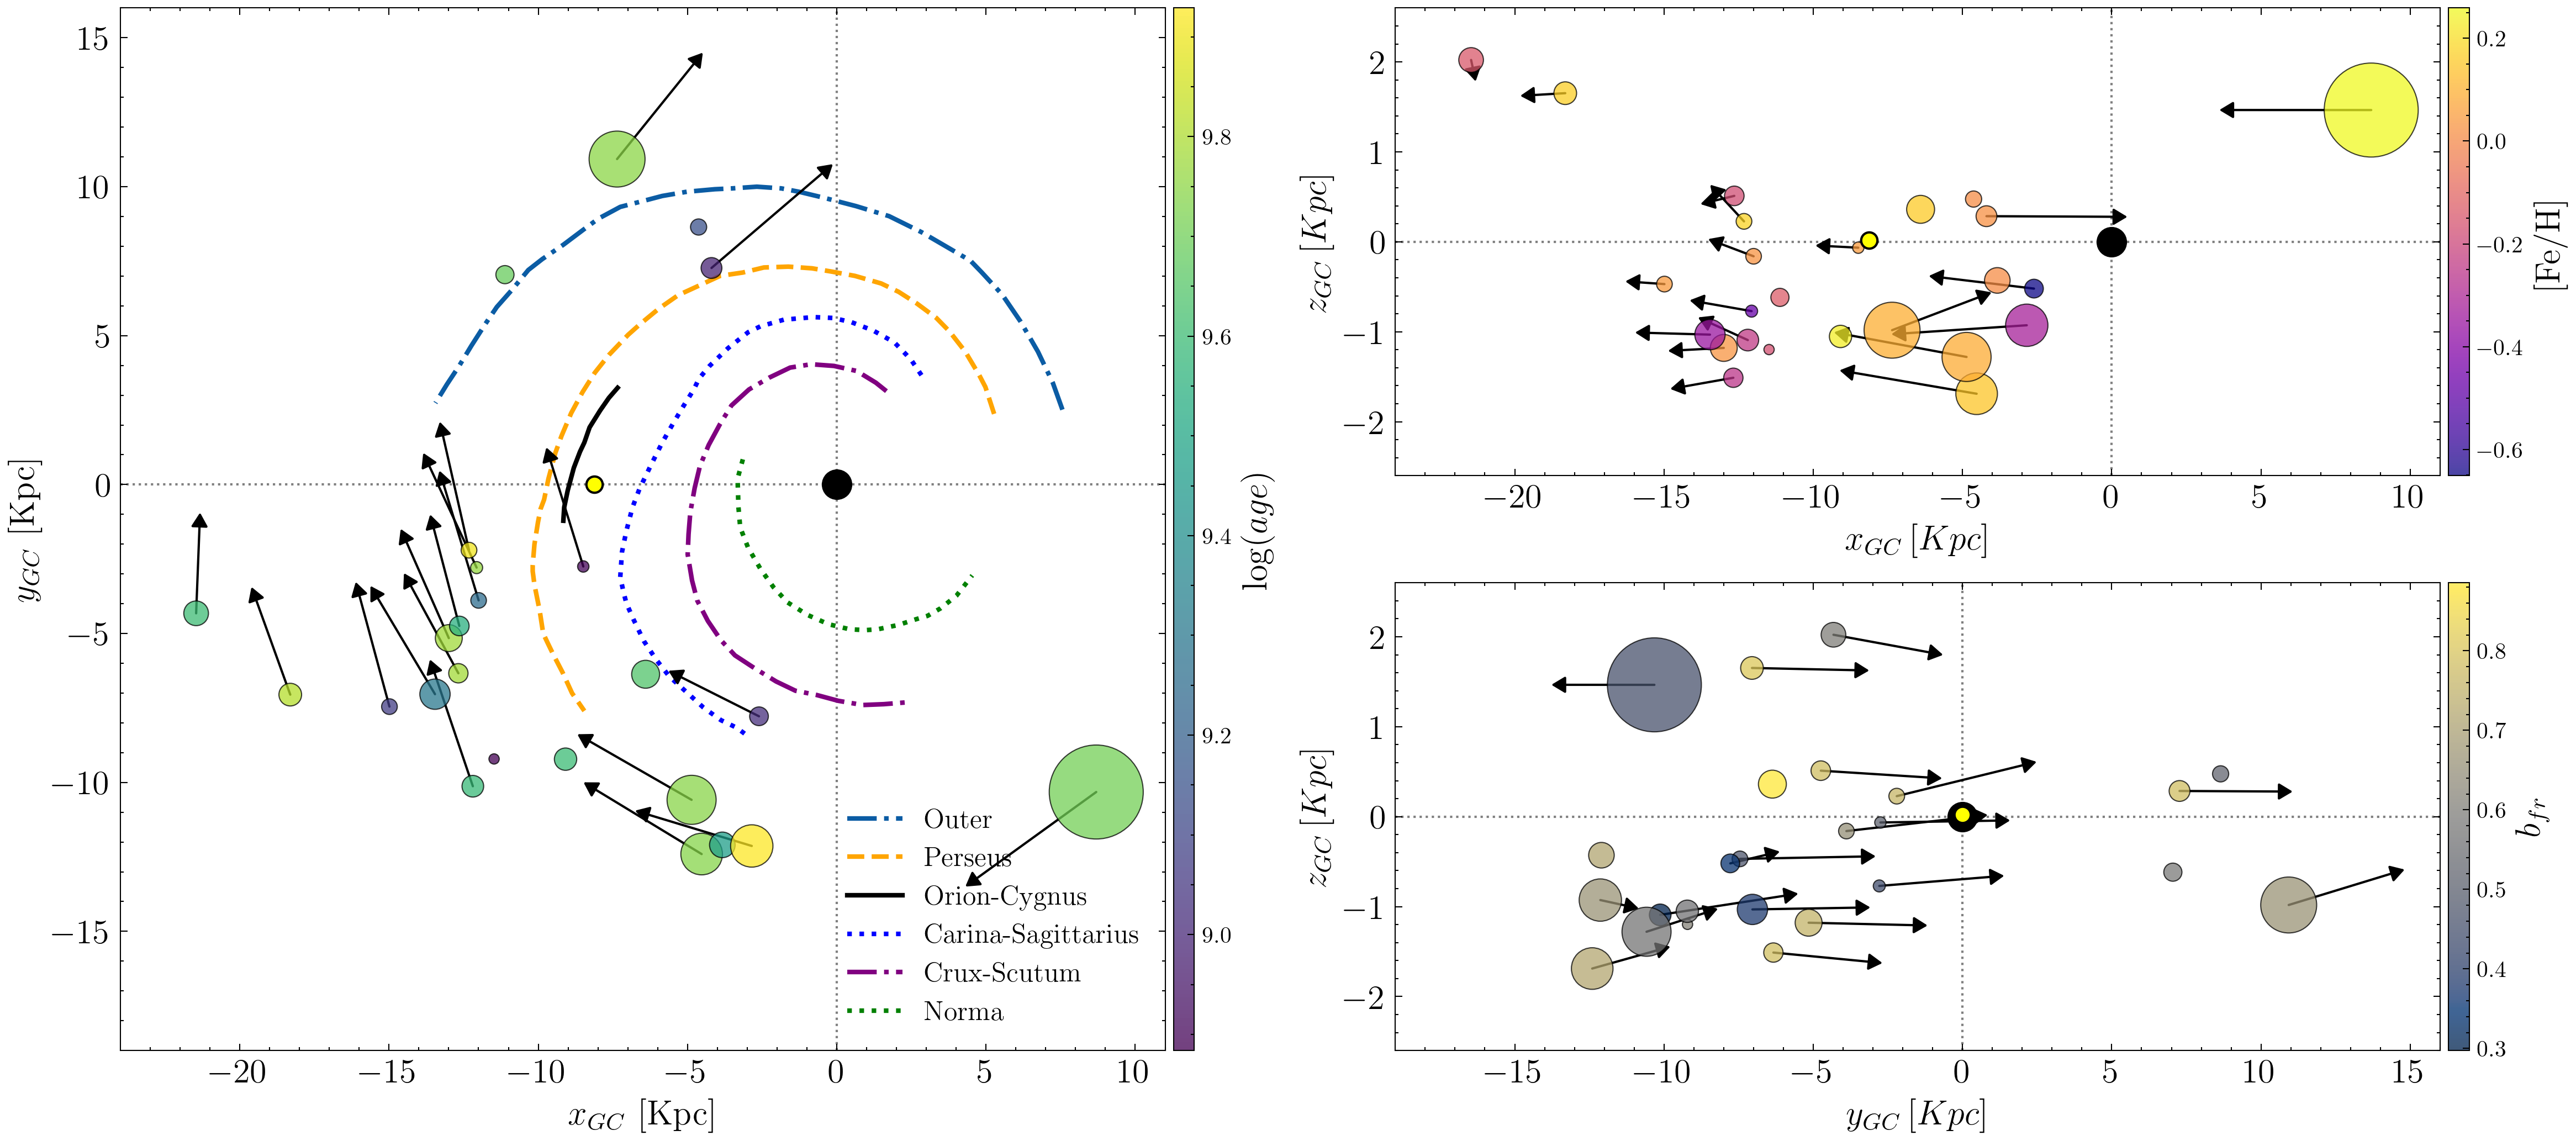
\includegraphics[]{figs/MWmap_AS.png}}
   \caption{xxx}
   \label{fig:MWmap_vectors}
  \end{figure*}






 \subsection{Metallicity gradient}
  \label{ssec:met_gradient}

  The radial metallicity ([Fe/H]) distribution, or metallicity gradient, is a
  key tracer of the Galaxy's chemical evolution. Open clusters have been used as
  a tool to investigate this relation for several decades~\citep{Janes_1979}.
  Although we have a somewhat small sample, we present here the results to
  highlight the 

  \cite{Donor_2020}, 

  Six of the clusters in our sample were investigated in~\cite{Netopil_2021} in
  relation with the metallicity gradient: BER25, BER29, BER73, CZER30, SAU1,
  and TOMB2.

  Three where studied in~\cite{Spina_2021}: BER29, BER73, CZER30
  [Fe/H]: -0.48 (1), -0.319 (1), -0.396 (2)
  (parenthesis: number of cluster members)


  \begin{figure}
   \resizebox{\hsize}{!}{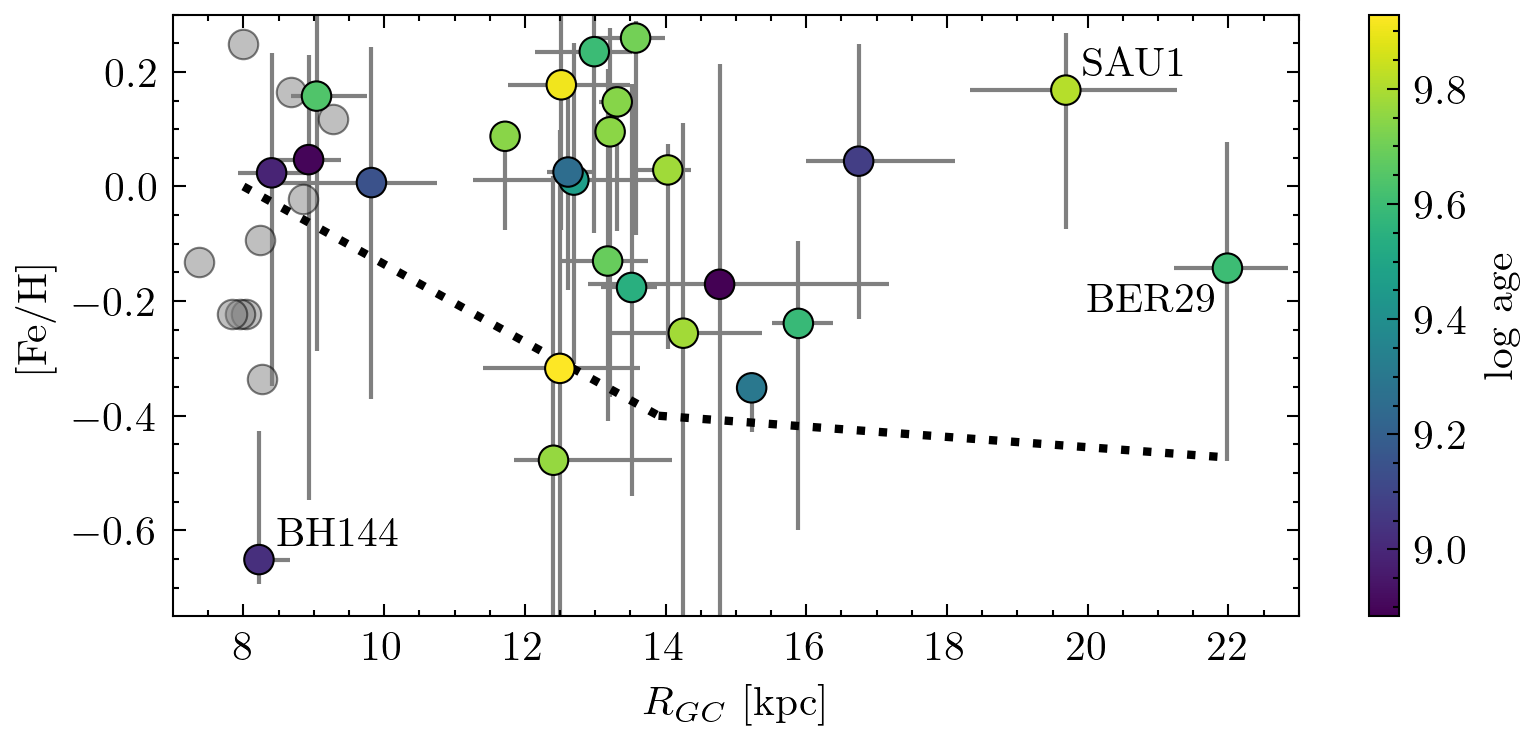
\includegraphics[]{figs/Fe_vs_R.png}}
   \caption{Metallicity gradient for the set of twenty-five analyzed clusters.
   Points are colored according to the $\log(age)$. Grey vertical lines are the
   16th and 84th percentiles. The dotted line is the broken relation from 
   \citet[][Fig 7]{Donor_2020}. The grey dots are the ten verified clusters
   from~\cite{Perren_2020}.}
   \label{fig:met_gradient}
  \end{figure}

  \cite{Salaris_2004}

  \begin{figure}
   \resizebox{\hsize}{!}{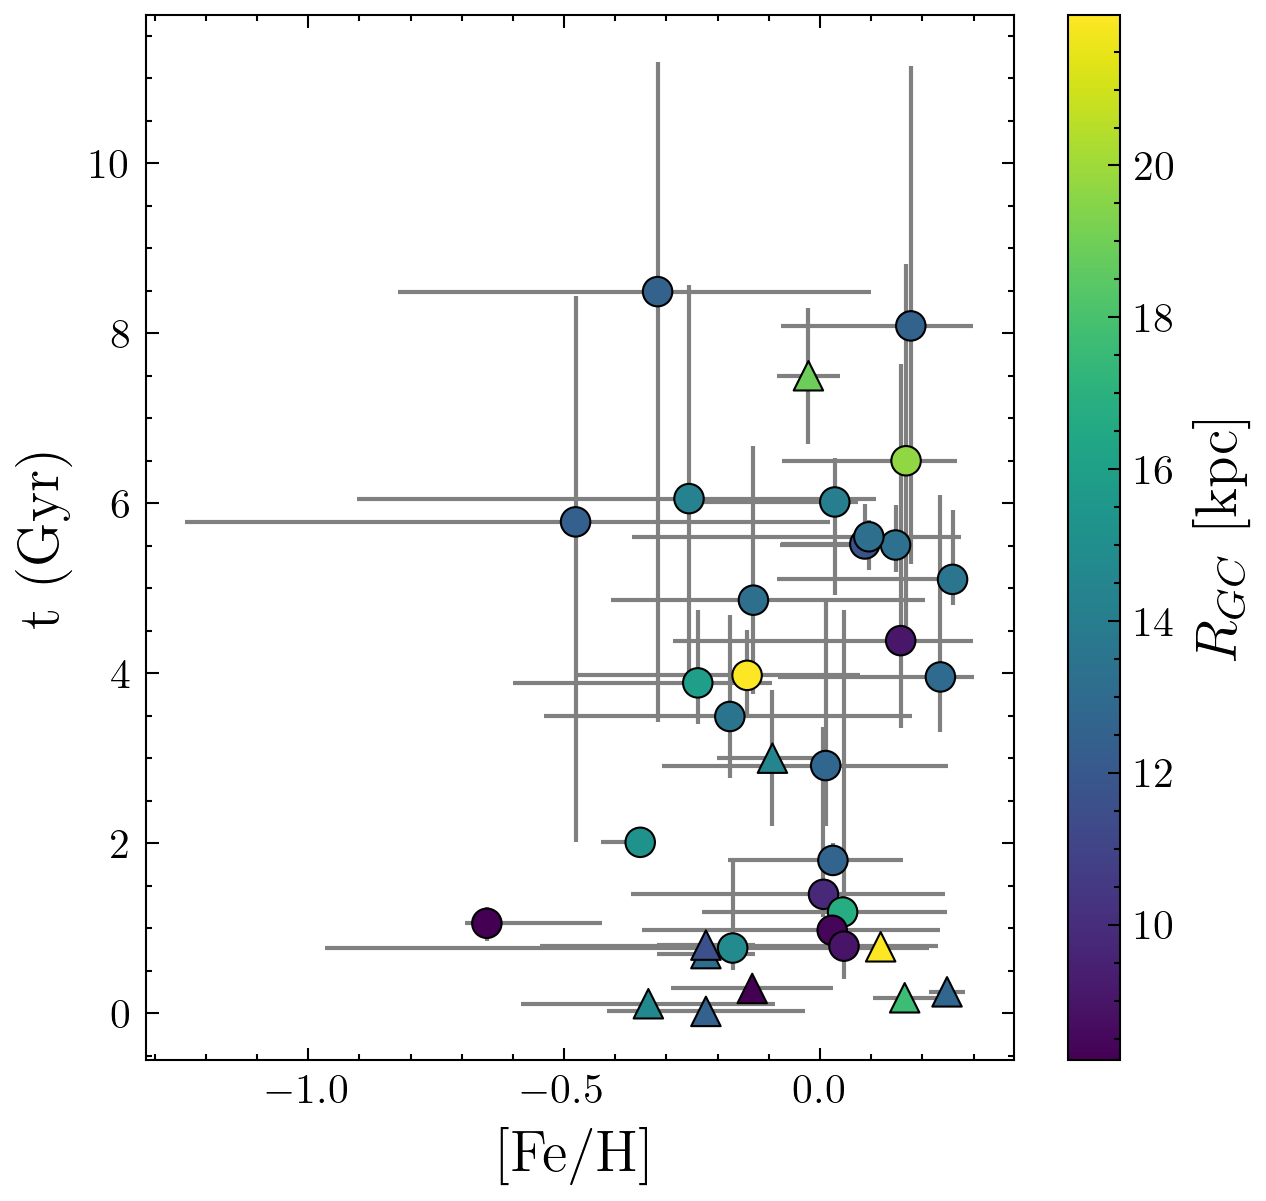
\includegraphics[]{figs/age_vs_Fe_H.png}}
   \caption{xxx}
   \label{fig:age_vs_feh}
  \end{figure}




 \subsection{Distances and distribution in the Galaxy.}
The fundamental parameters of the 25 clusters in our sample have been reassessed
using pyUPMASK and ASteCA. The results are shown in Table 3. Inspecting the data
in the table we see that none of them is a young cluster. Indeed, with the
exception of just two, the remaining ones are older than 1 Gyr. 13 clusters out
of 25 are at more than 9 kpc from the sun, thus reducing the sample found in
data bases in almost one half. 
In terms of the galacto-centric distance, RG, and distribution in the galactic
plane it happens that 14 are placed in the third galactic quadrant and 10 out of
these 14 are under the formal galactic equator at negative latitudes. The other
4 above the galactic plane are, Berkeley 26 at 12.52 kpc, Saurer 1 at 19.69 kpc,
Cz30 at 13.52 and Berk 29 at 21.98 kpc.  Berkeley 26, one of the oldest cluster
in our sample is found at z= 0.2 kpc. The most distant cluster in this quadrant,
Berk29, appears at z=2 kpc above the formal galactic plane while Saurer 1 has z
near 1.65 kpc and CZER 30 is at z=0.51 kpc.  At first glance, we are tempted to
think that a large number of clusters in the third quadrant seems to accompany
the warp defined by diffuse blue population(references are needed) which maximum
height above the plane takes place at about -8 in latitude and near 240 in longitude.
(Esto debo completarlo…).
But more interesting is to see five clusters are farther than the assumed limit
for the galactic disk radius (van referencias). They are: Berkeley 29, Rgc=22 kpc,
Tombaugh 2, Rg=15, F1212 at Rg= 16 kpc,  SAU1 with Rg= 19 kpc and ARPM2 at
Rg= 16 kpc. These numbers, if confirmed, may imply that the galaxy disc may be
larger than assumed.\\

 When comparing our results in Table 3 with those coming from the MWSC, WEBDA,
Open Cclus and Cantat-Gaudin databases, we clearly see important disagreements
in almost all the parameters. We show in Fig. xx our distances against those
given in each database;  just for easing things we indicated the ages of the
clusters obtained  by us using a color scale. The best overall agreement in
distances is found with Cantat-Gaudin for 16 clusters in common with differences
ranging from -2000 to +3000 parsecs without appearing to be any dependency on
the age of the clusters.  Within the limits of the associated errors, we can
affirm that the agreement with CG is reasonably good.  Differences with other
authors are frequently huge spanning a range from -10 to +10 kpc. 

\subsection{The ages}
Regarding the ages that come out from our analysis scheme, we see in Fig. Xx that
ASteCA shows a systematic tendency to estimate older ages in comparison with all
the databases, although the effect is quite smaller in the case of clusters in
common with CG. The exception is Berkeley 37, in which case the difference to CG
is very large. 

We see systematic effects regarding age differences in the sense that our values
tend to be larger. There must have a superimposition of reasons to produce that
effect. With CG there are 6 cluster showing such differences and this can may be
due to a different treatment of binarity (a free parameter in our analysis).



\subsection{Velocities}



\subsection{The metal content}




% =============================================================================
\section{Conclusions}
 \label{sec:conclusions}


 xxx






% =============================================================================

\begin{acknowledgements}
G.I.P., M.S.P., and R.A.V. acknowledge the financial support from CONICET 
(PIP317) and the UNLP (PID-G148 project).
%
This work has made use of data from the European Space Agency (ESA) mission
{\it Gaia} (\url{https://www.cosmos.esa.int/gaia}), processed by the {\it Gaia}
Data Processing and Analysis Consortium (DPAC,
\url{https://www.cosmos.esa.int/web/gaia/dpac/consortium}). Funding for the DPAC
has been provided by national institutions, in particular the institutions
participating in the {\it Gaia} Multilateral Agreement.
%
This research has made use of the WEBDA database, operated at the Department of
Theoretical Physics and Astrophysics of the Masaryk University.
%
This research has made use of the VizieR catalog access tool, operated at CDS,
Strasbourg, France~\citep{Ochsenbein_2000}.
%
This research has made use of ``Aladin sky atlas'' developed at
CDS, Strasbourg Observatory, France~\citep{Bonnarel2000,Boch2014}.
%
This research has made use of NASA's Astrophysics Data System.
%
This research made use of the Python language v3.7.3~\citep{vanRossum_1995}
and the following packages:
NumPy\footnote{\url{http://www.numpy.org/}}~\citep{vanDerWalt_2011};
SciPy\footnote{\url{http://www.scipy.org/}}~\citep{Jones_2001};
Astropy\footnote{\url{http://www.astropy.org/}}, a community-developed core
Python package for Astronomy \citep{astropy:2013, astropy:2018};
matplotlib\footnote{\url{http://matplotlib.org/}}~\citep{hunter_2007};
scikit-learn\footnote{\url{https://scikit-learn.org/}}~\citep{scikit-learn};
\texttt{ASteCA}\footnote{\url{https://github.com/asteca}};
ptemcee\footnote{\url{https://github.com/willvousden/ptemcee}};
Kalkayotl\footnote{\url{https://github.com/olivares-j/Kalkayotl}};
sfdmap\footnote{\url{https://github.com/kbarbary/sfdmap}}
\end{acknowledgements}




\bibliographystyle{aa}
\bibliography{biblio} % your references Yourfile.bib


\begin{appendix}
\section{Structure analysis}
\label{app:struct_analysis}


 \begin{table}
 \caption{Core ($r_{c}$), tidal ($r_{t}$), and adopted ($r_{a}$) radii values.
 The first two are shown with their respective 16th an 84th percentiles in
 parenthesis.}
 \label{tab:radii}
 \centering
 \begin{tabular}{llll}
 \hline\hline
 Cluster & $r_{c}$ (16th, 84th) &  $r_{t}$ (16th, 84th) & $r_{a}$\\
 \hline
  BER73         & 0.6 (0.5, 0.7) &  4.9 (3.8, 6.3) &  2.0\\
  BER25         & 1.5 (1.2, 1.8) &  7.0 (6.2, 8.0) &  5.0\\
  BER75         & 0.4 (0.3, 0.5) &  5.0 (3.6, 6.6) &  2.0\\
  BER26         & 0.7 (0.5, 1.0) &  3.4 (2.5, 4.5) &  1.6\\
  BER29         & 0.5 (0.4, 0.5) &  7.4 (6.4, 8.6) &  3.0\\
  TOMB2         & 0.9 (0.8, 0.9) &  6.7 (6.1, 7.4) &  3.5\\
  BER76         & 1.6 (1.2, 2.5) &  7.4 (5.7, 9.6) &  4.0\\
  F1212         & 0.8 (0.6, 1.1) &  8.8 (6.6, 10.7) & 3.0\\
  SAU1          & 0.7 (0.5, 1.0) &  3.9 (2.9, 5.4) &  2.0\\
  CZER30        & 0.6 (0.4, 0.7) &  6.4 (4.8, 8.2) &  2.5\\
  ARPM2         & 1.4 (1.0, 2.0) &  4.1 (3.4, 4.9) &  3.0\\
  BH4           & 0.4 (0.3, 0.5) &  5.7 (4.0, 7.1) &  2.0\\
  F1419         & 1.2 (0.9, 1.8) &  6.0 (4.3, 8.3) &  3.0\\
  BH37          & 1.2 (0.8, 1.9) &  3.8 (2.5, 5.6) &  2.0\\
  E9205         & 1.0 (0.9, 1.3) &  4.4 (3.7, 5.3) &  3.0\\
  E9218         & 0.6 (0.6, 0.7) &  6.5 (5.9, 7.3) &  3.0\\
  SAU3          & 0.5 (0.4, 0.6) &  4.9 (3.8, 6.4) &  2.0\\
  KRON39        & 0.3 (0.2, 0.3) &  5.6 (4.1, 7.0) &  2.0\\
  E9308         & 0.2 (0.2, 0.2) &  5.0 (4.2, 5.7) &  1.5\\
  BH144         & 0.3 (0.3, 0.4) &  2.8 (2.3, 3.4) &  1.5\\
  BH176         & 0.6 (0.5, 0.7) &  4.6 (3.8, 5.8) &  2.0\\
  KRON31        & 0.5 (0.4, 0.6) &  6.9 (5.7, 7.6) &  2.0\\
  SAU6          & 0.5 (0.4, 0.7) &  3.7 (2.9, 4.8) &  2.0\\
  BER56         & 1.6 (1.4, 1.7) &  8.1 (7.4, 8.9) &  4.5\\
  BER102        & 1.0 (0.8, 1.5) &  3.8 (3.0, 4.9) &  2.5\\
  % BER73         & 0.6$_{0.5}^{0.7}$ &  4.9$_{3.8}^{6.3}$ &  2.0\\
  % BER25         & 1.5$_{1.2}^{1.8}$ &  7.0$_{6.2}^{8.0}$ &  5.0\\
  % BER75         & 0.4$_{0.3}^{0.5}$ &  5.0$_{3.6}^{6.6}$ &  2.0\\
  % BER26         & 0.7$_{0.5}^{1.0}$ &  3.4$_{2.5}^{4.5}$ &  1.6\\
  % BER29         & 0.5$_{0.4}^{0.5}$ &  7.4$_{6.4}^{8.6}$ &  3.0\\
  % TOMB2         & 0.9$_{0.8}^{0.9}$ &  6.7$_{6.1}^{7.4}$ &  3.5\\
  % BER76         & 1.6$_{1.2}^{2.5}$ &  7.4$_{5.7}^{9.6}$ &  4.0\\
  % F1212         & 0.8$_{0.6}^{1.1}$ &  8.8$_{6.6}^{10.7}$ & 3.0\\
  % SAU1          & 0.7$_{0.5}^{1.0}$ &  3.9$_{2.9}^{5.4}$ &  2.0\\
  % CZER30        & 0.6$_{0.4}^{0.7}$ &  6.4$_{4.8}^{8.2}$ &  2.5\\
  % ARPM2         & 1.4$_{1.0}^{2.0}$ &  4.1$_{3.4}^{4.9}$ &  3.0\\
  % BH4           & 0.4$_{0.3}^{0.5}$ &  5.7$_{4.0}^{7.1}$ &  2.0\\
  % F1419         & 1.2$_{0.9}^{1.8}$ &  6.0$_{4.3}^{8.3}$ &  3.0\\
  % BH37          & 1.2$_{0.8}^{1.9}$ &  3.8$_{2.5}^{5.6}$ &  2.0\\
  % E9205         & 1.0$_{0.9}^{1.3}$ &  4.4$_{3.7}^{5.3}$ &  3.0\\
  % E9218         & 0.6$_{0.6}^{0.7}$ &  6.5$_{5.9}^{7.3}$ &  3.0\\
  % SAU3          & 0.5$_{0.4}^{0.6}$ &  4.9$_{3.8}^{6.4}$ &  2.0\\
  % KRON39        & 0.3$_{0.2}^{0.3}$ &  5.6$_{4.1}^{7.0}$ &  2.0\\
  % E9308         & 0.2$_{0.2}^{0.2}$ &  5.0$_{4.2}^{5.7}$ &  1.5\\
  % BH144         & 0.3$_{0.3}^{0.4}$ &  2.8$_{2.3}^{3.4}$ &  1.5\\
  % BH176         & 0.6$_{0.5}^{0.7}$ &  4.6$_{3.8}^{5.8}$ &  2.0\\
  % KRON31        & 0.5$_{0.4}^{0.6}$ &  6.9$_{5.7}^{7.6}$ &  2.0\\
  % SAU6          & 0.5$_{0.4}^{0.7}$ &  3.7$_{2.9}^{4.8}$ &  2.0\\
  % BER56         & 1.6$_{1.4}^{1.7}$ &  8.1$_{7.4}^{8.9}$ &  4.5\\
  % BER102        & 1.0$_{0.8}^{1.5}$ &  3.8$_{3.0}^{4.9}$ &  2.5\\
 \hline
 \end{tabular}
 \end{table}

 \begin{figure*}
  \resizebox{\hsize}{!}{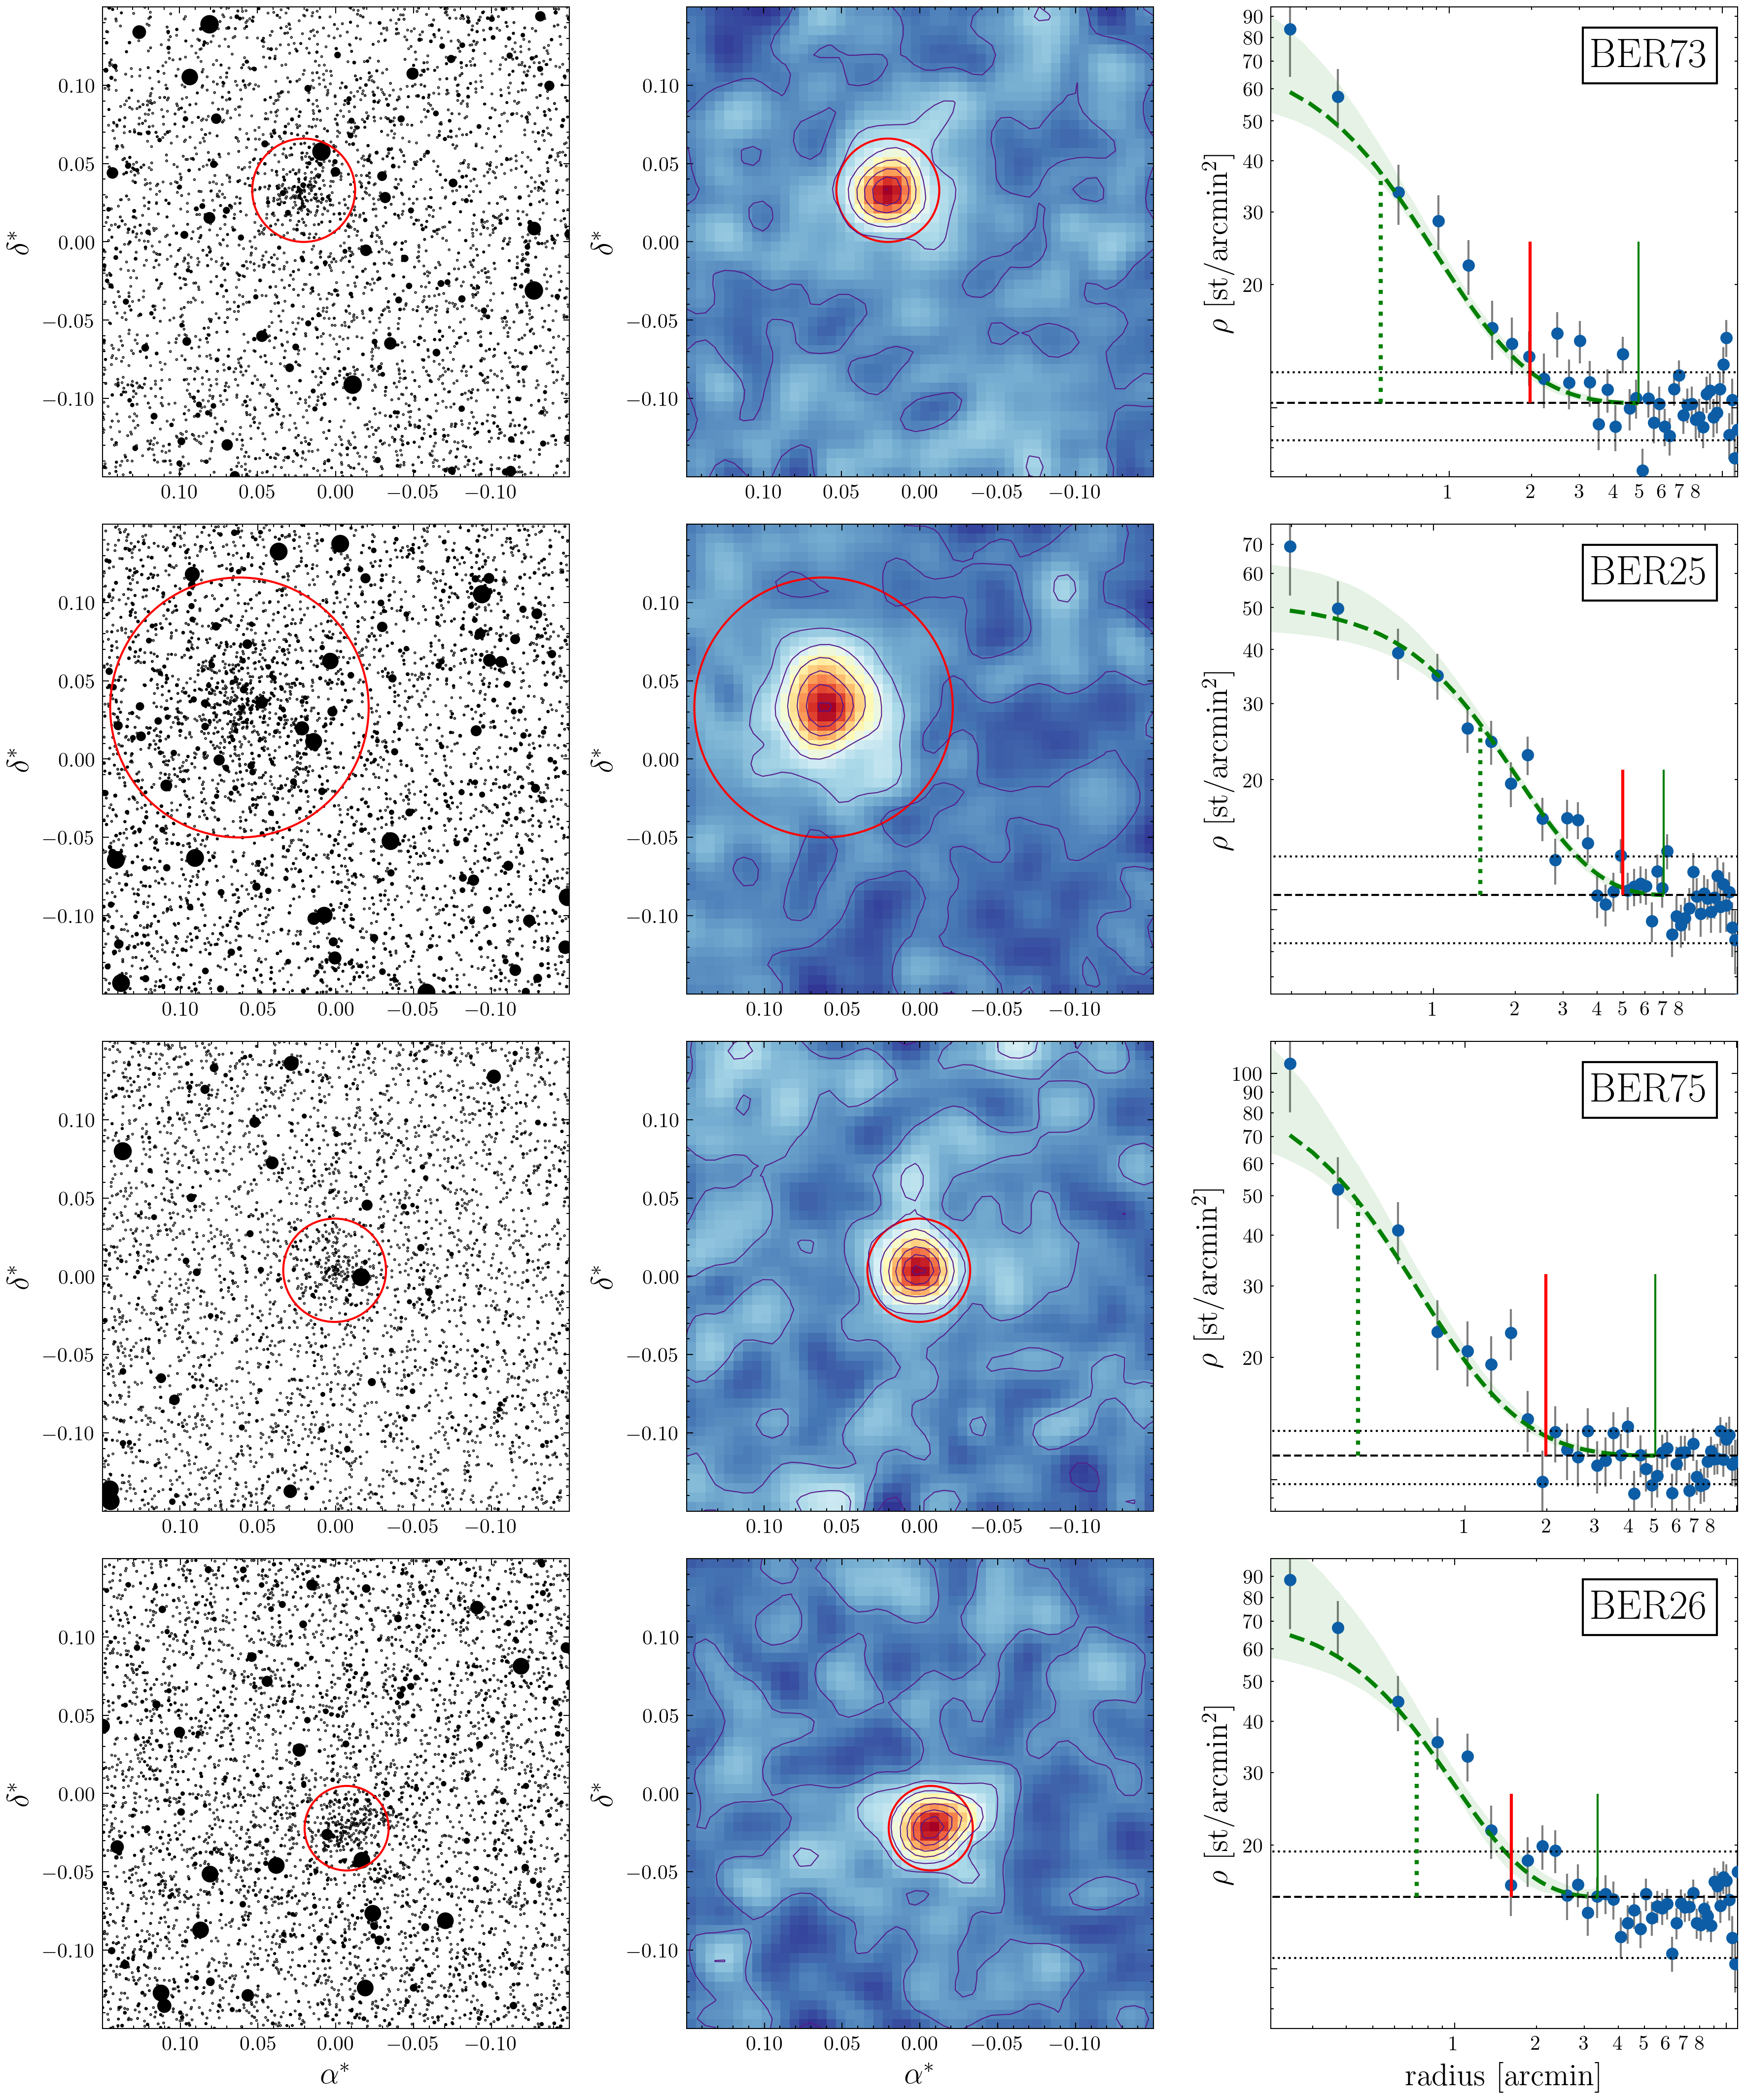
\includegraphics[]{figs/0_struct.png}}
  \caption{xxx}
  \label{fig:0struct}
 \end{figure*}

 \begin{figure*}
  \resizebox{\hsize}{!}{\includegraphics[]{figs/4_struct.png}}
  \caption{xxx}
  \label{fig:4struct}
 \end{figure*}

 \begin{figure*}
  \resizebox{\hsize}{!}{\includegraphics[]{figs/8_struct.png}}
  \caption{xxx}
  \label{fig:8struct}
 \end{figure*}

 \begin{figure*}
  \resizebox{\hsize}{!}{\includegraphics[]{figs/12_struct.png}}
  \caption{xxx}
  \label{fig:12struct}
 \end{figure*}

 \begin{figure*}
  \resizebox{\hsize}{!}{\includegraphics[]{figs/16_struct.png}}
  \caption{xxx}
  \label{fig:16struct}
 \end{figure*}

 \begin{figure*}
  \resizebox{\hsize}{!}{\includegraphics[]{figs/20_struct.png}}
  \caption{xxx}
  \label{fig:20struct}
 \end{figure*}


\section{Fundamental parameters}
\label{app:fundam_params}

 \begin{figure*}[t]
  % \resizebox{\hsize}{!}{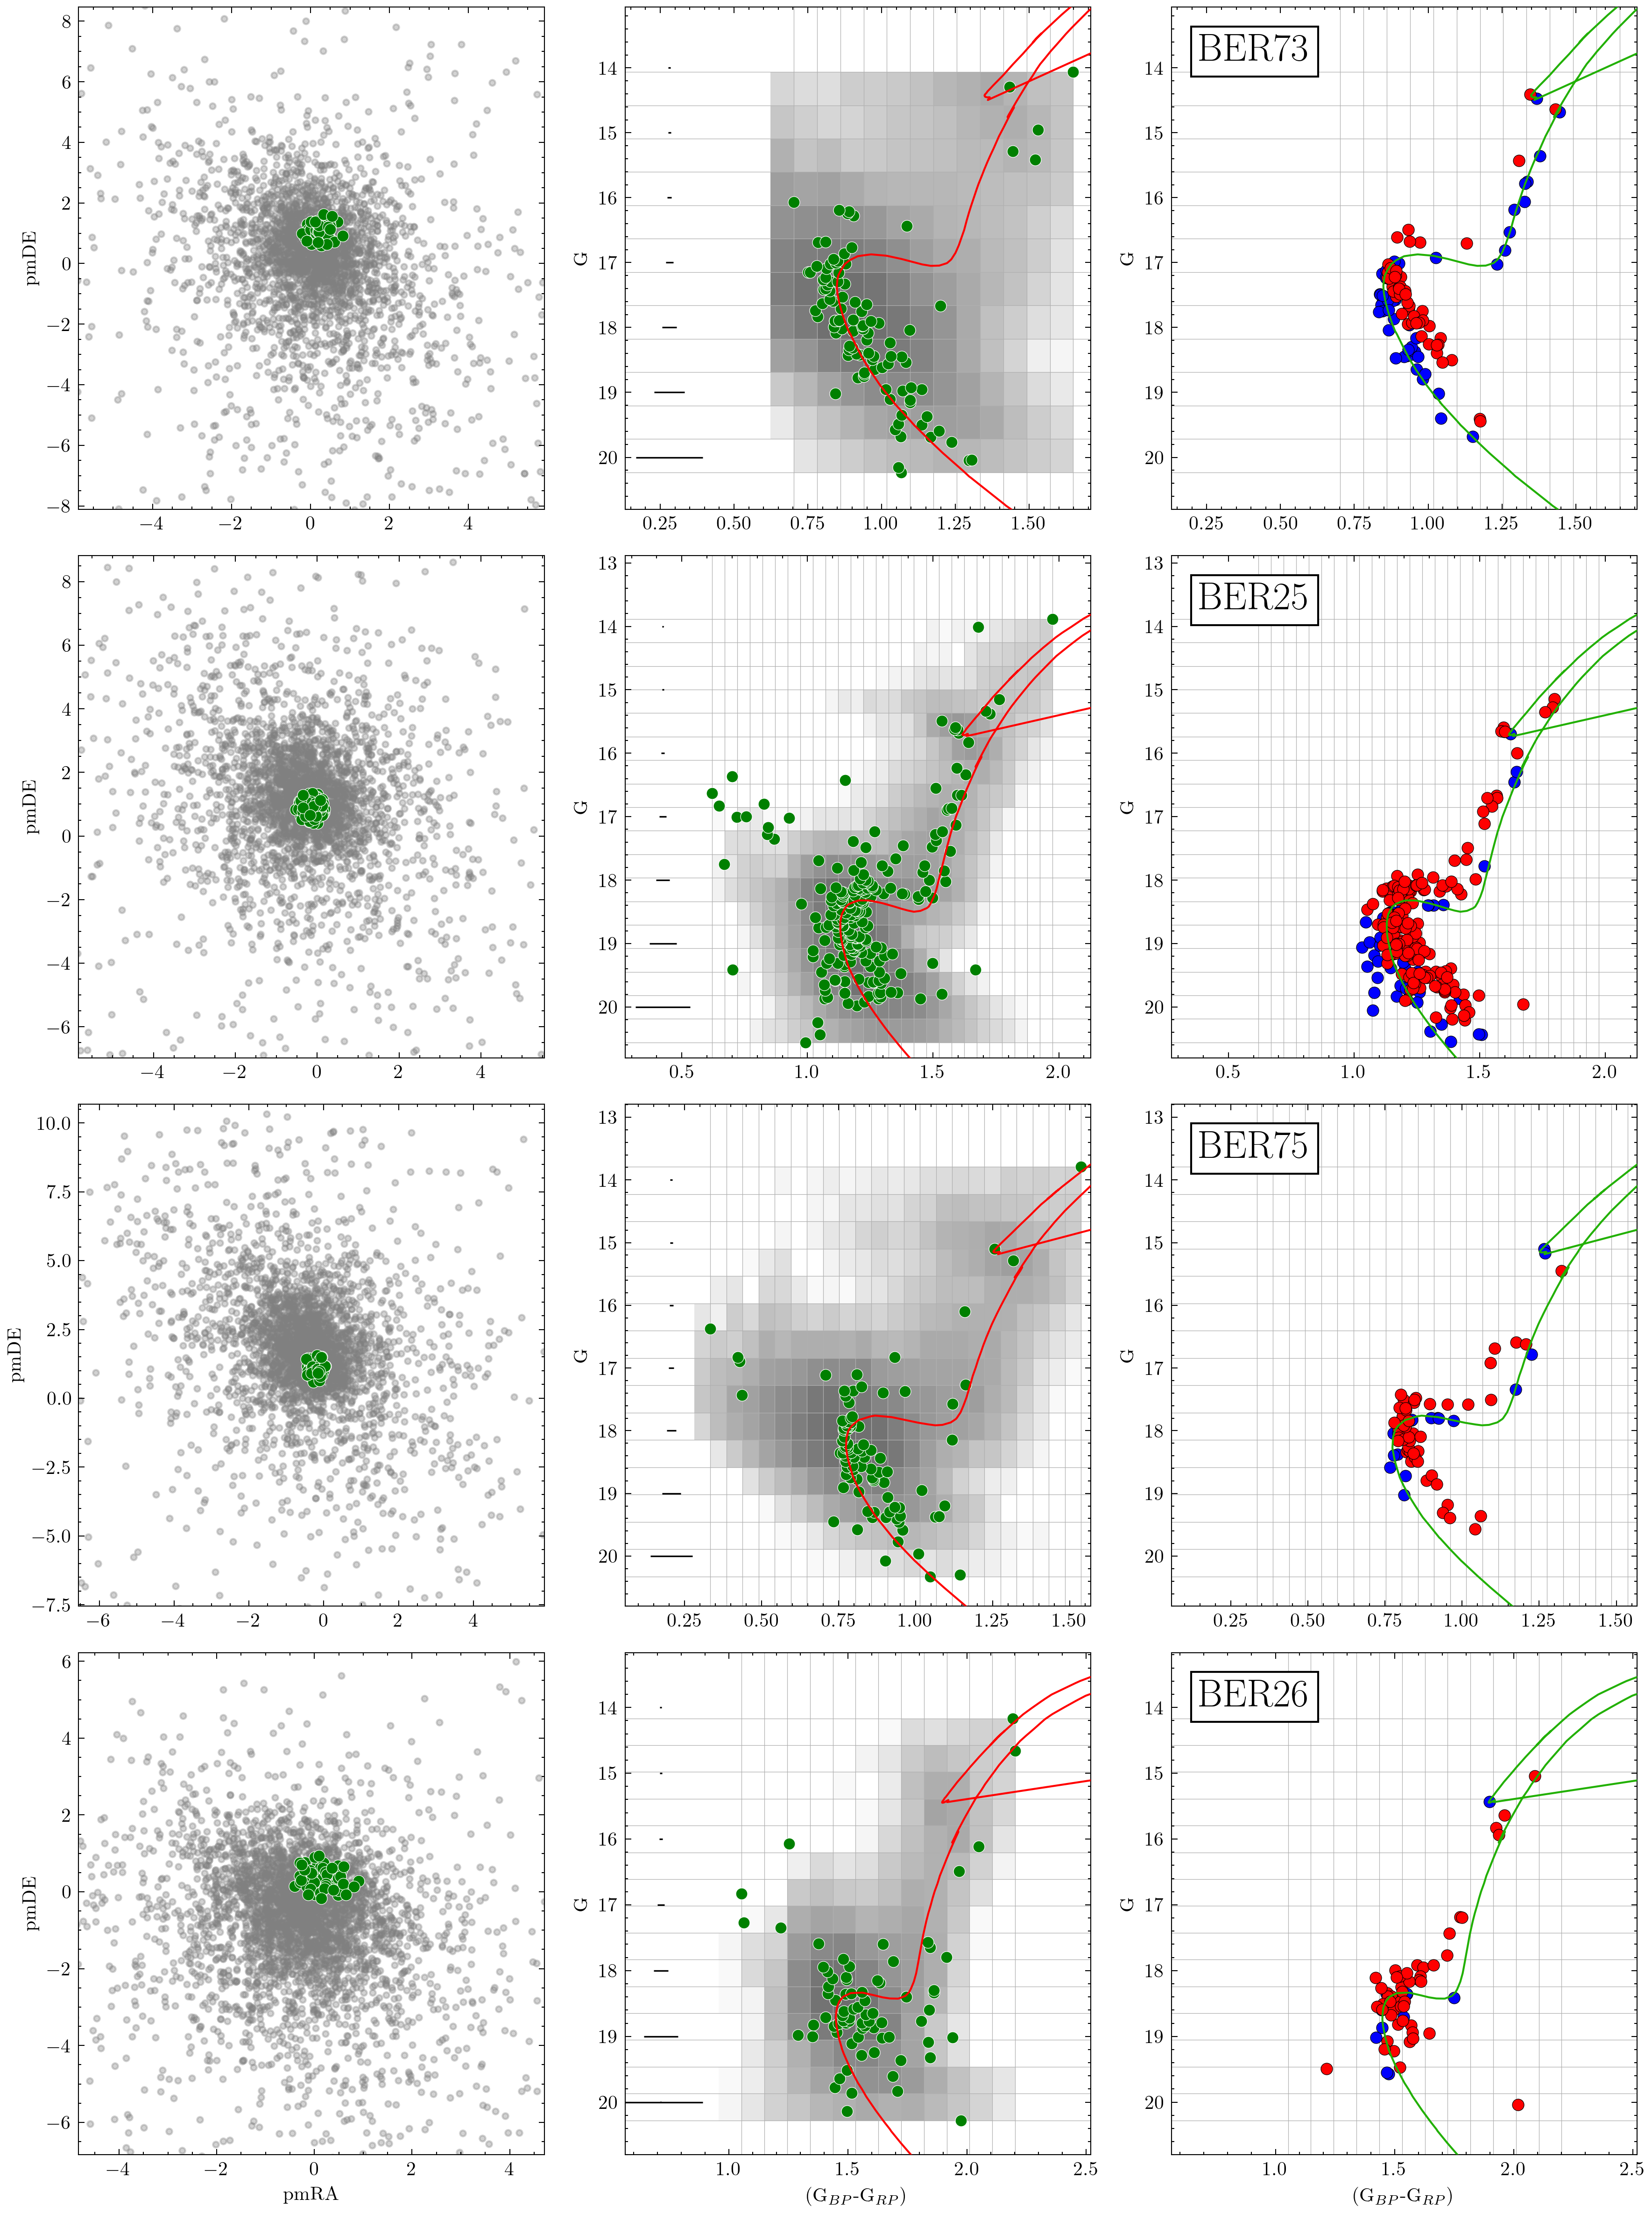
\includegraphics[height=.9\textheight]{figs/0_fpars.png}}
  \centering
  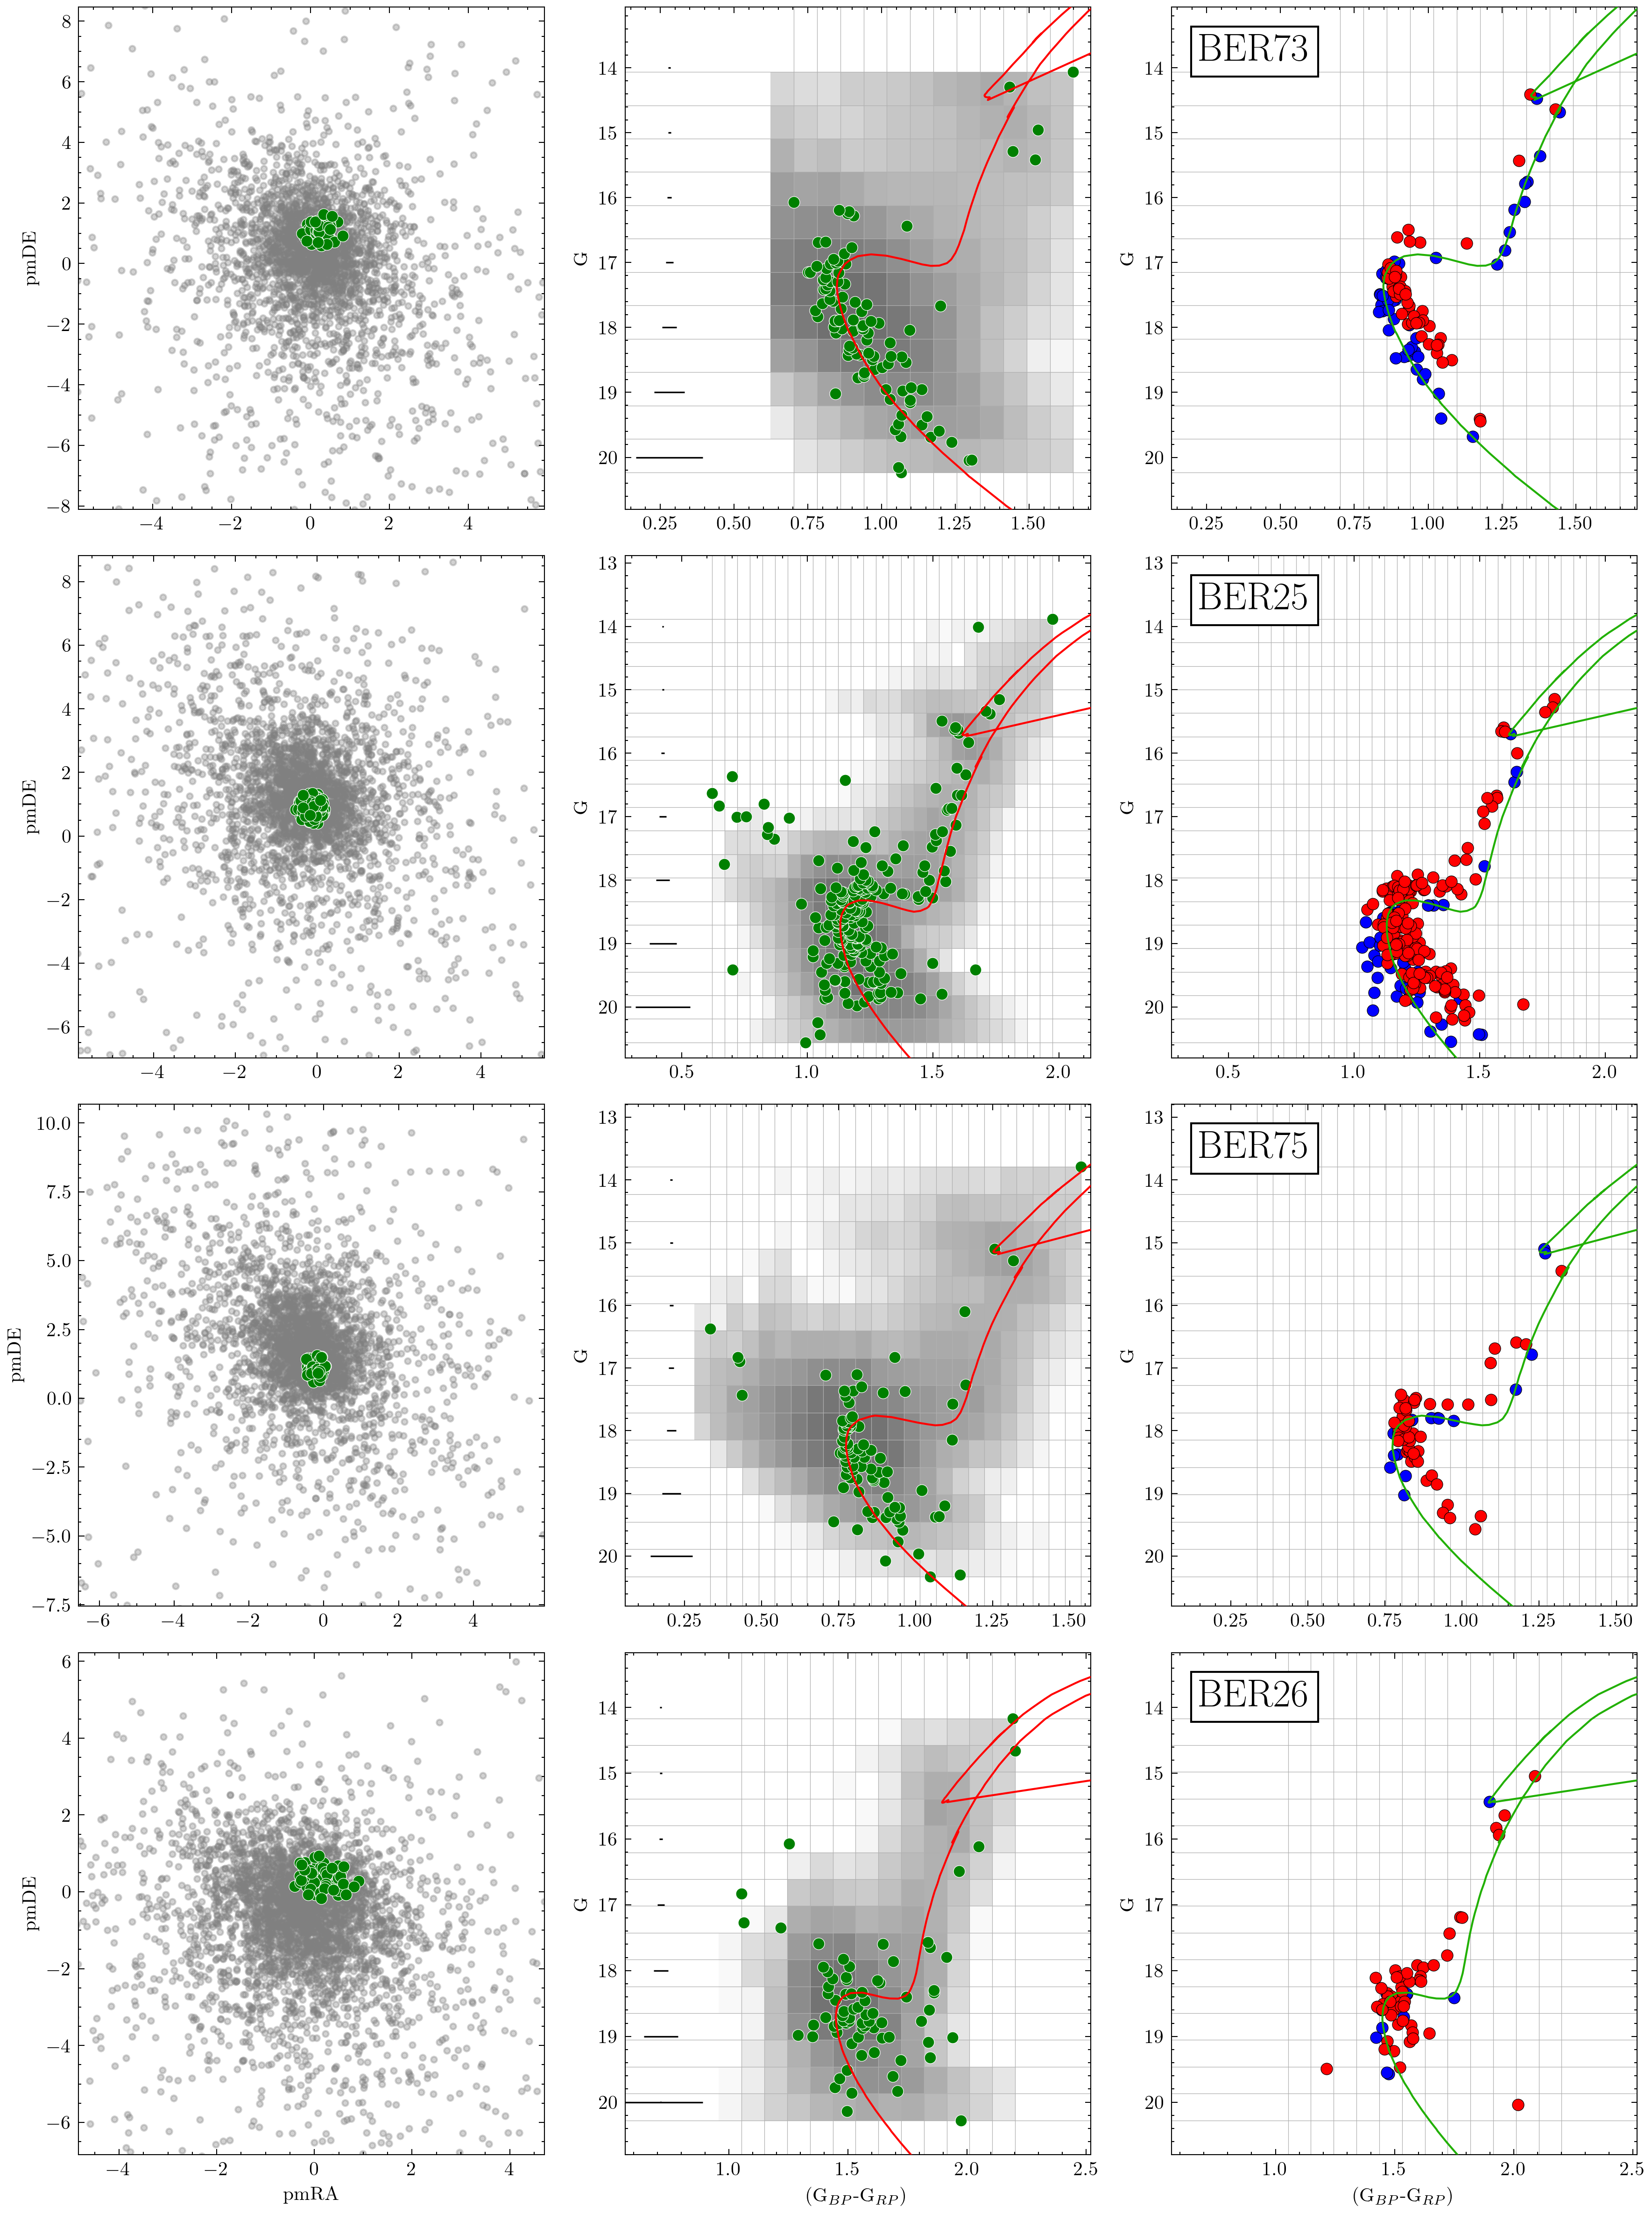
\includegraphics[height=.95\textheight]{figs/0_fpars.png}
  \caption{xxx}
  \label{fig:0fpars}
 \end{figure*}

 \begin{figure*}
  % \resizebox{\hsize}{!}{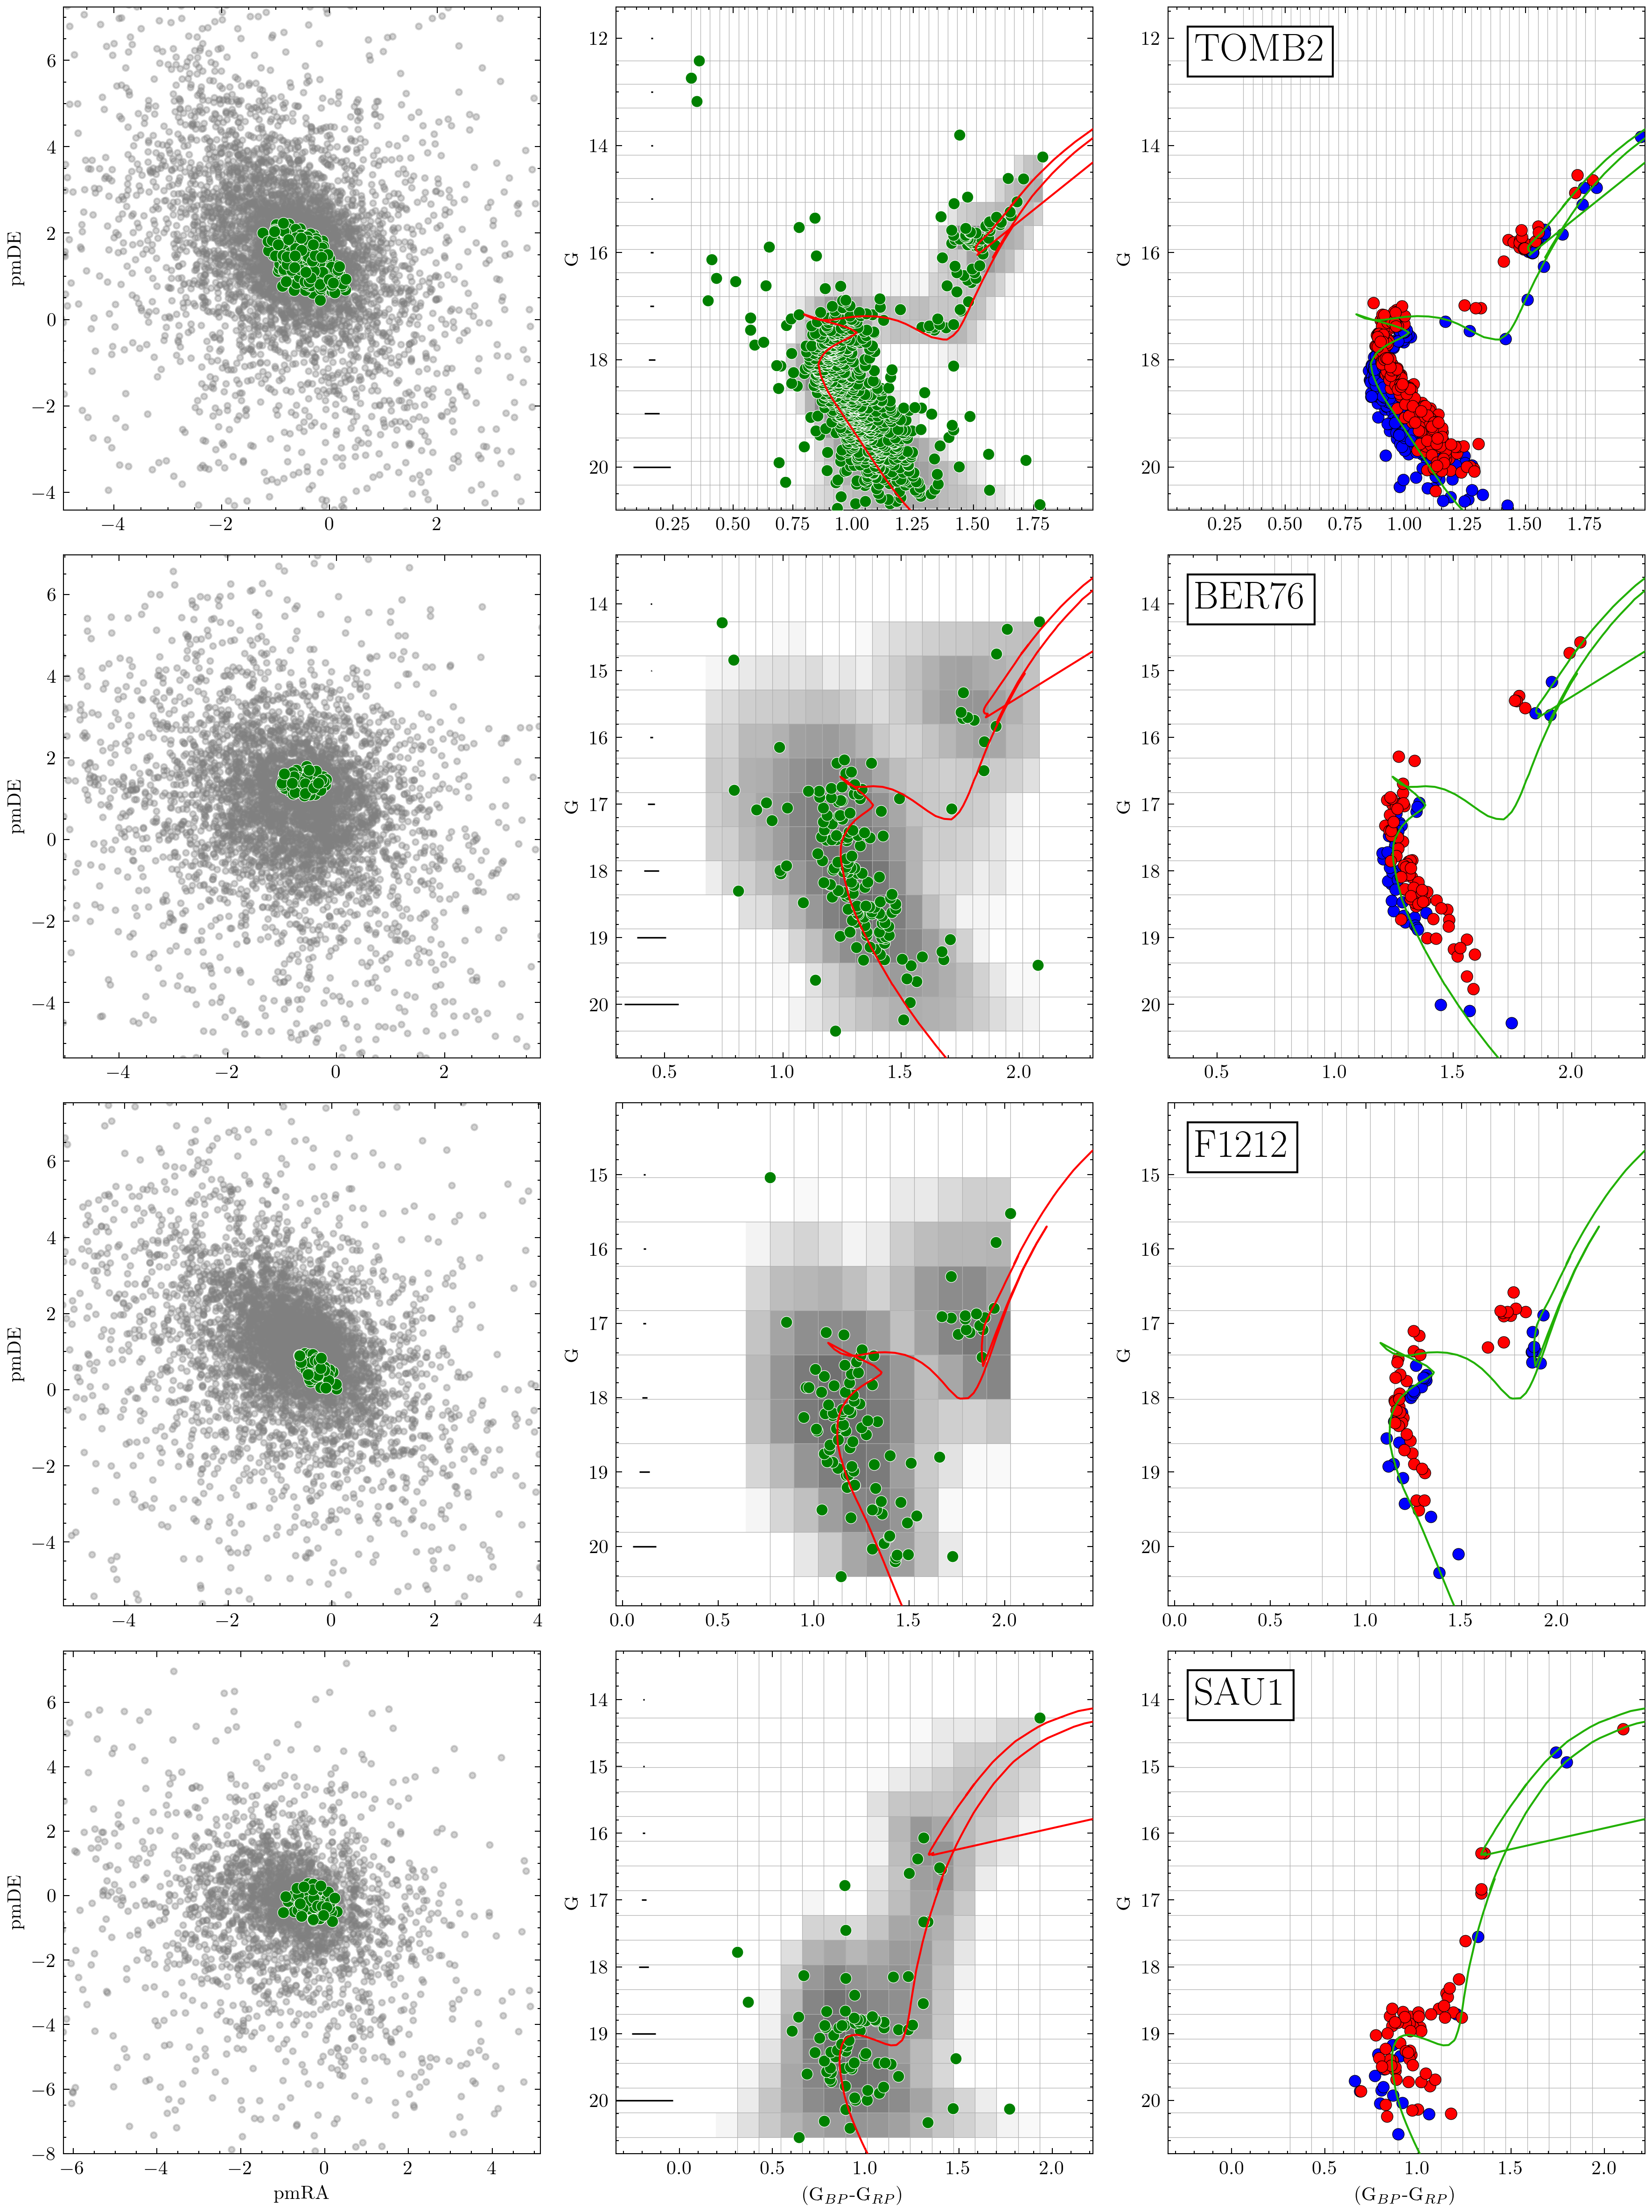
\includegraphics[height=.9\textheight]{figs/4_fpars.png}}
  \centering
  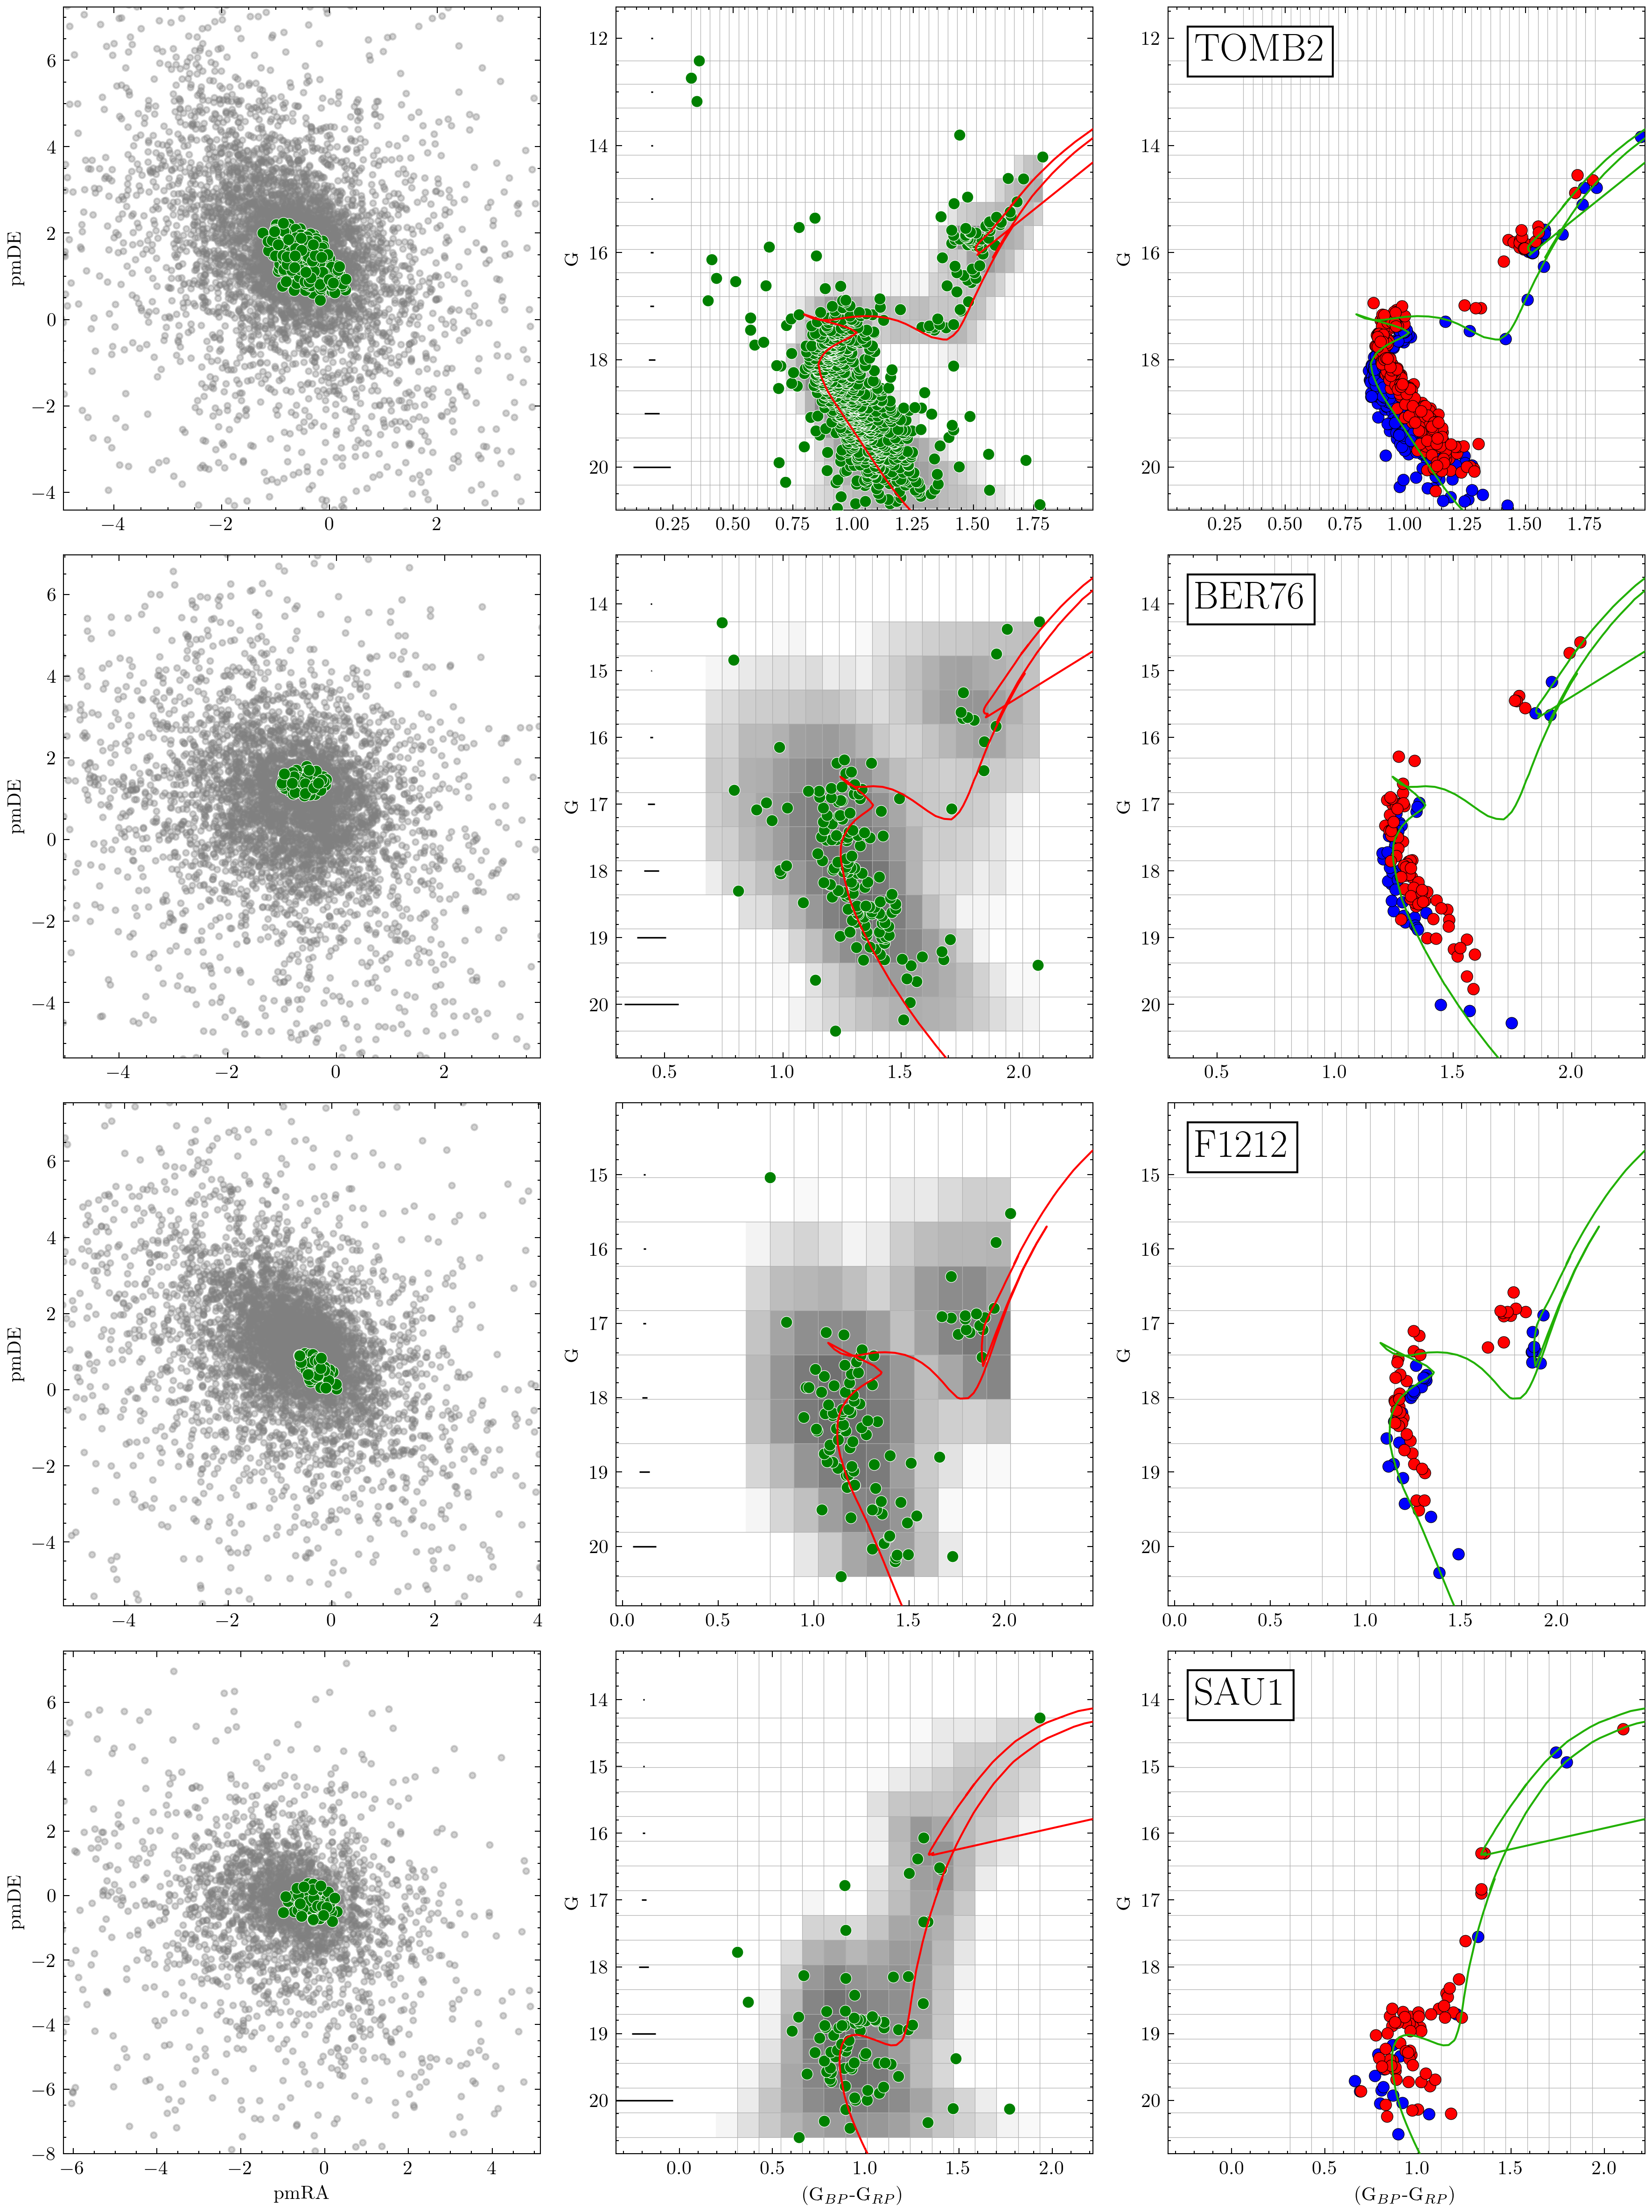
\includegraphics[height=.95\textheight]{figs/4_fpars.png}
  \caption{xxx}
  \label{fig:4fpars}
 \end{figure*}

 \begin{figure*}
  % \resizebox{\hsize}{!}{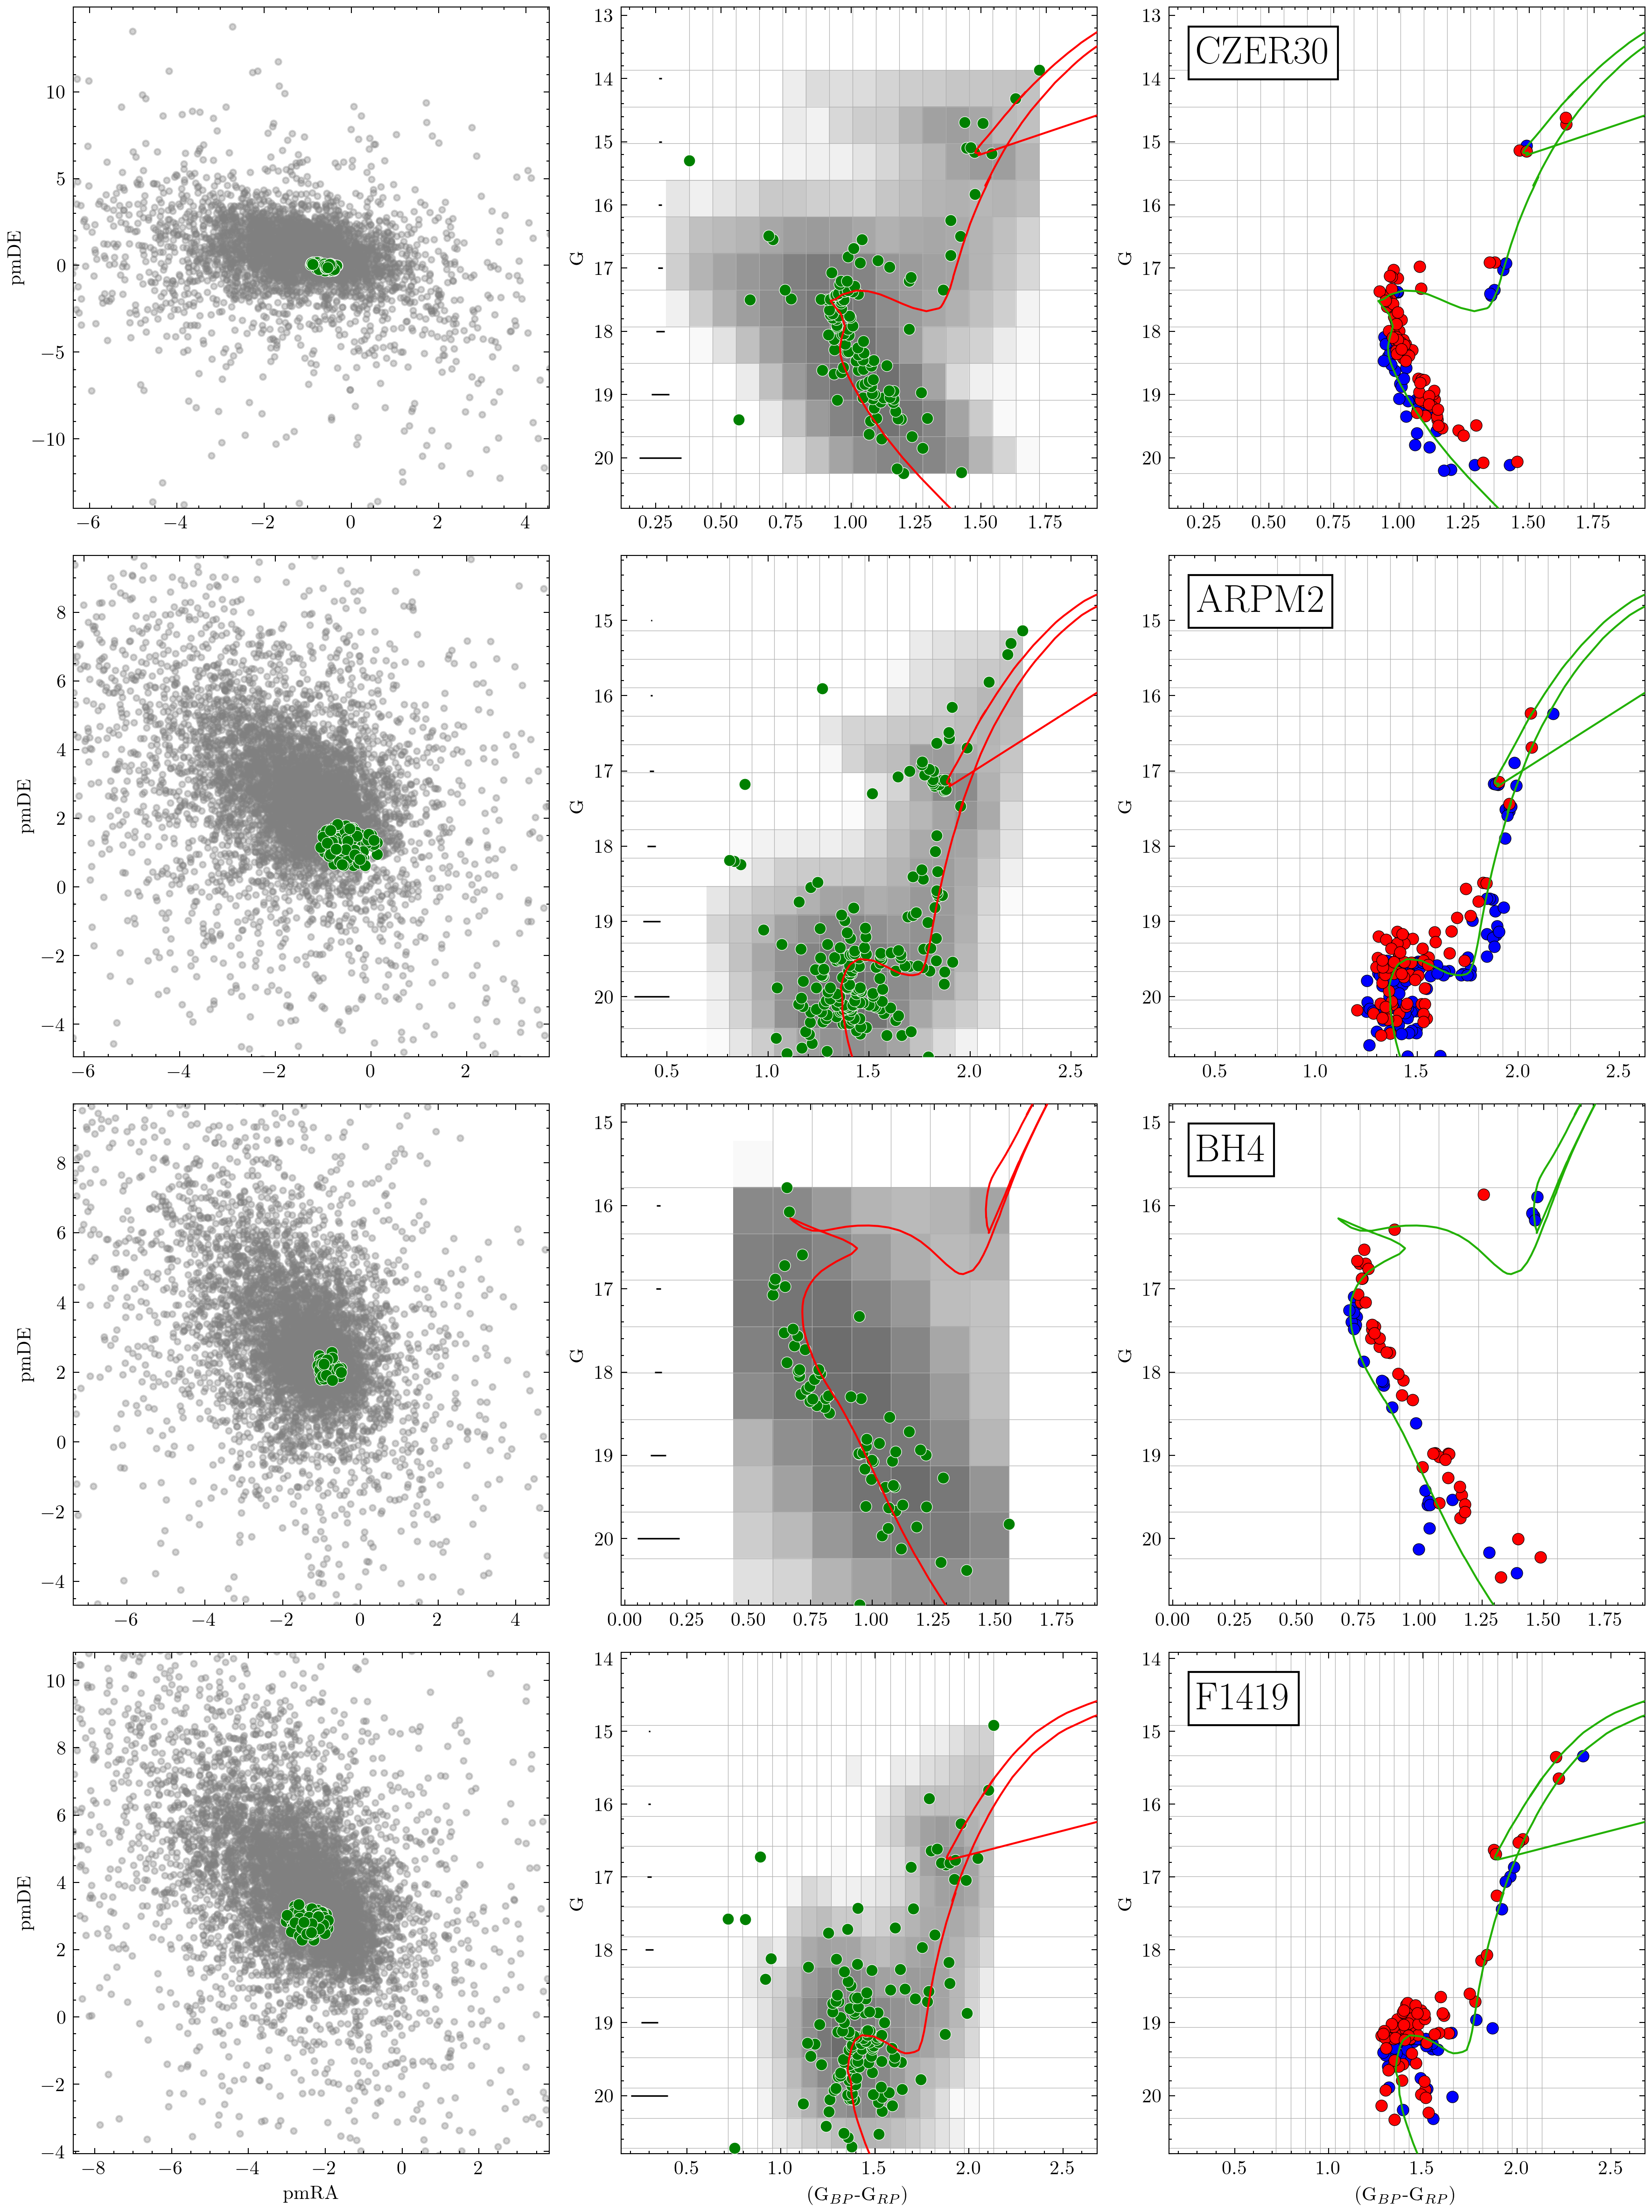
\includegraphics[height=.9\textheight]{figs/8_fpars.png}}
  \centering
  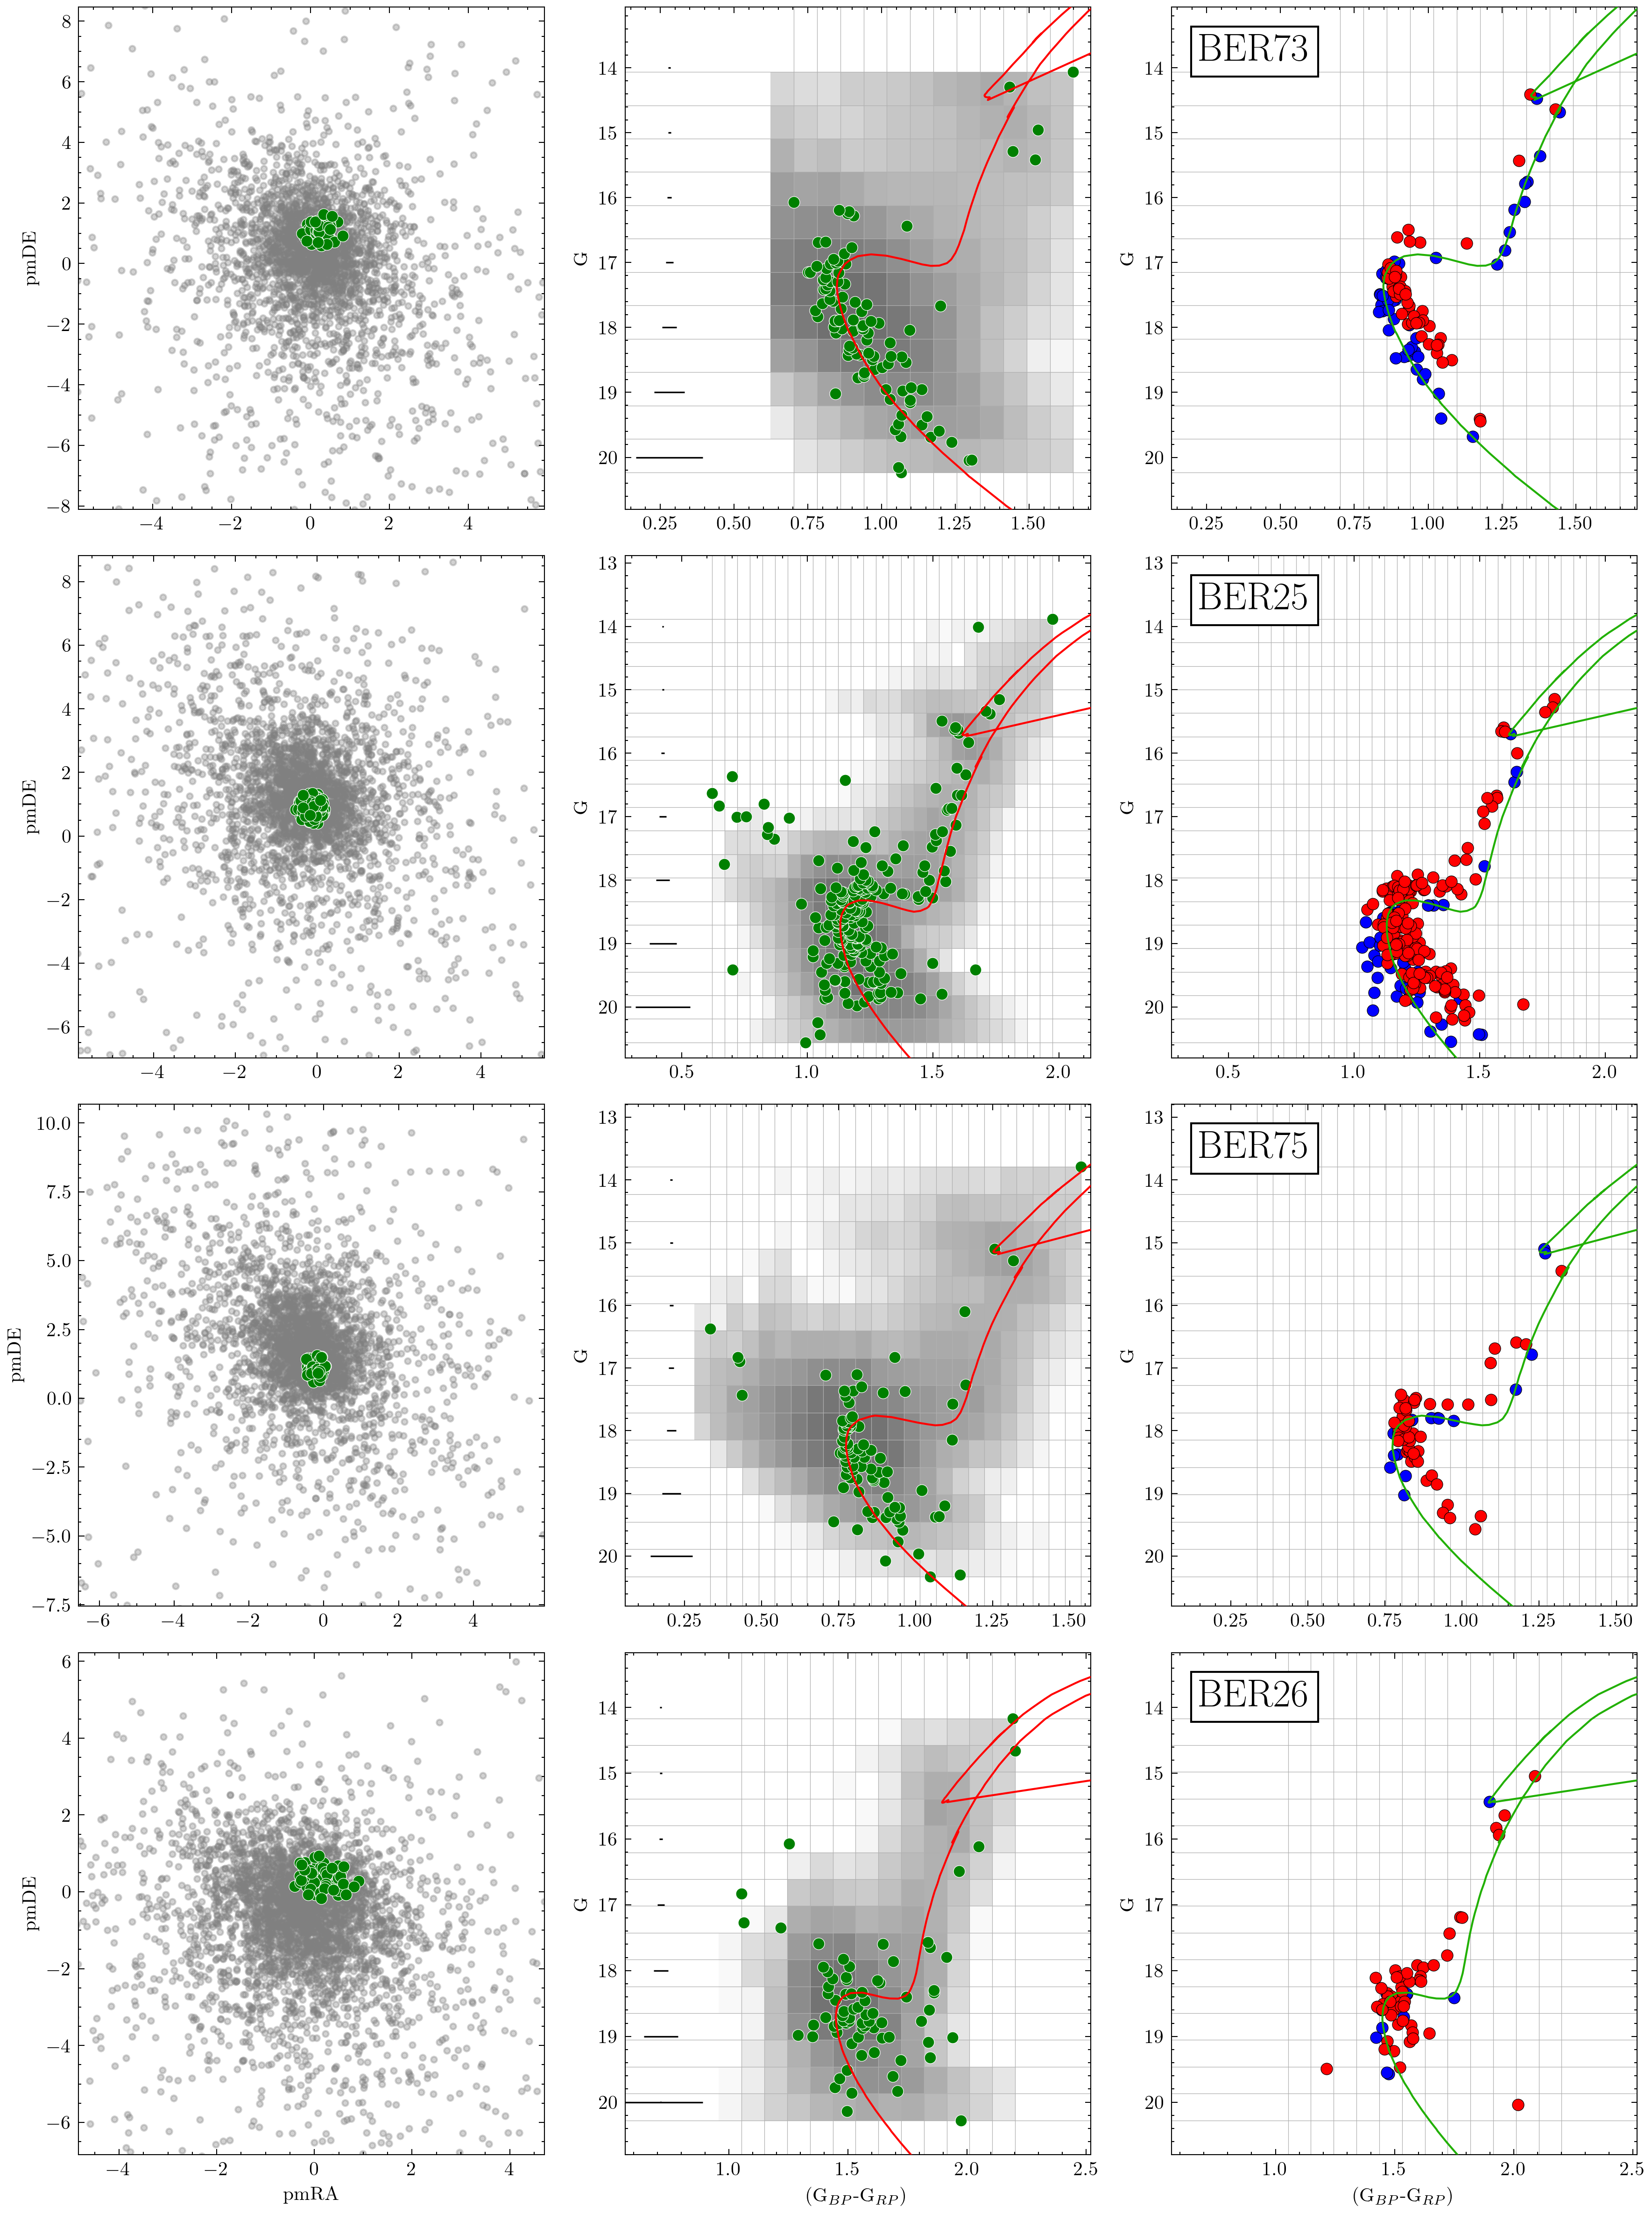
\includegraphics[height=.95\textheight]{figs/0_fpars.png}
  \caption{xxx}
  \label{fig:8fpars}
 \end{figure*}

 \begin{figure*}
  % \resizebox{\hsize}{!}{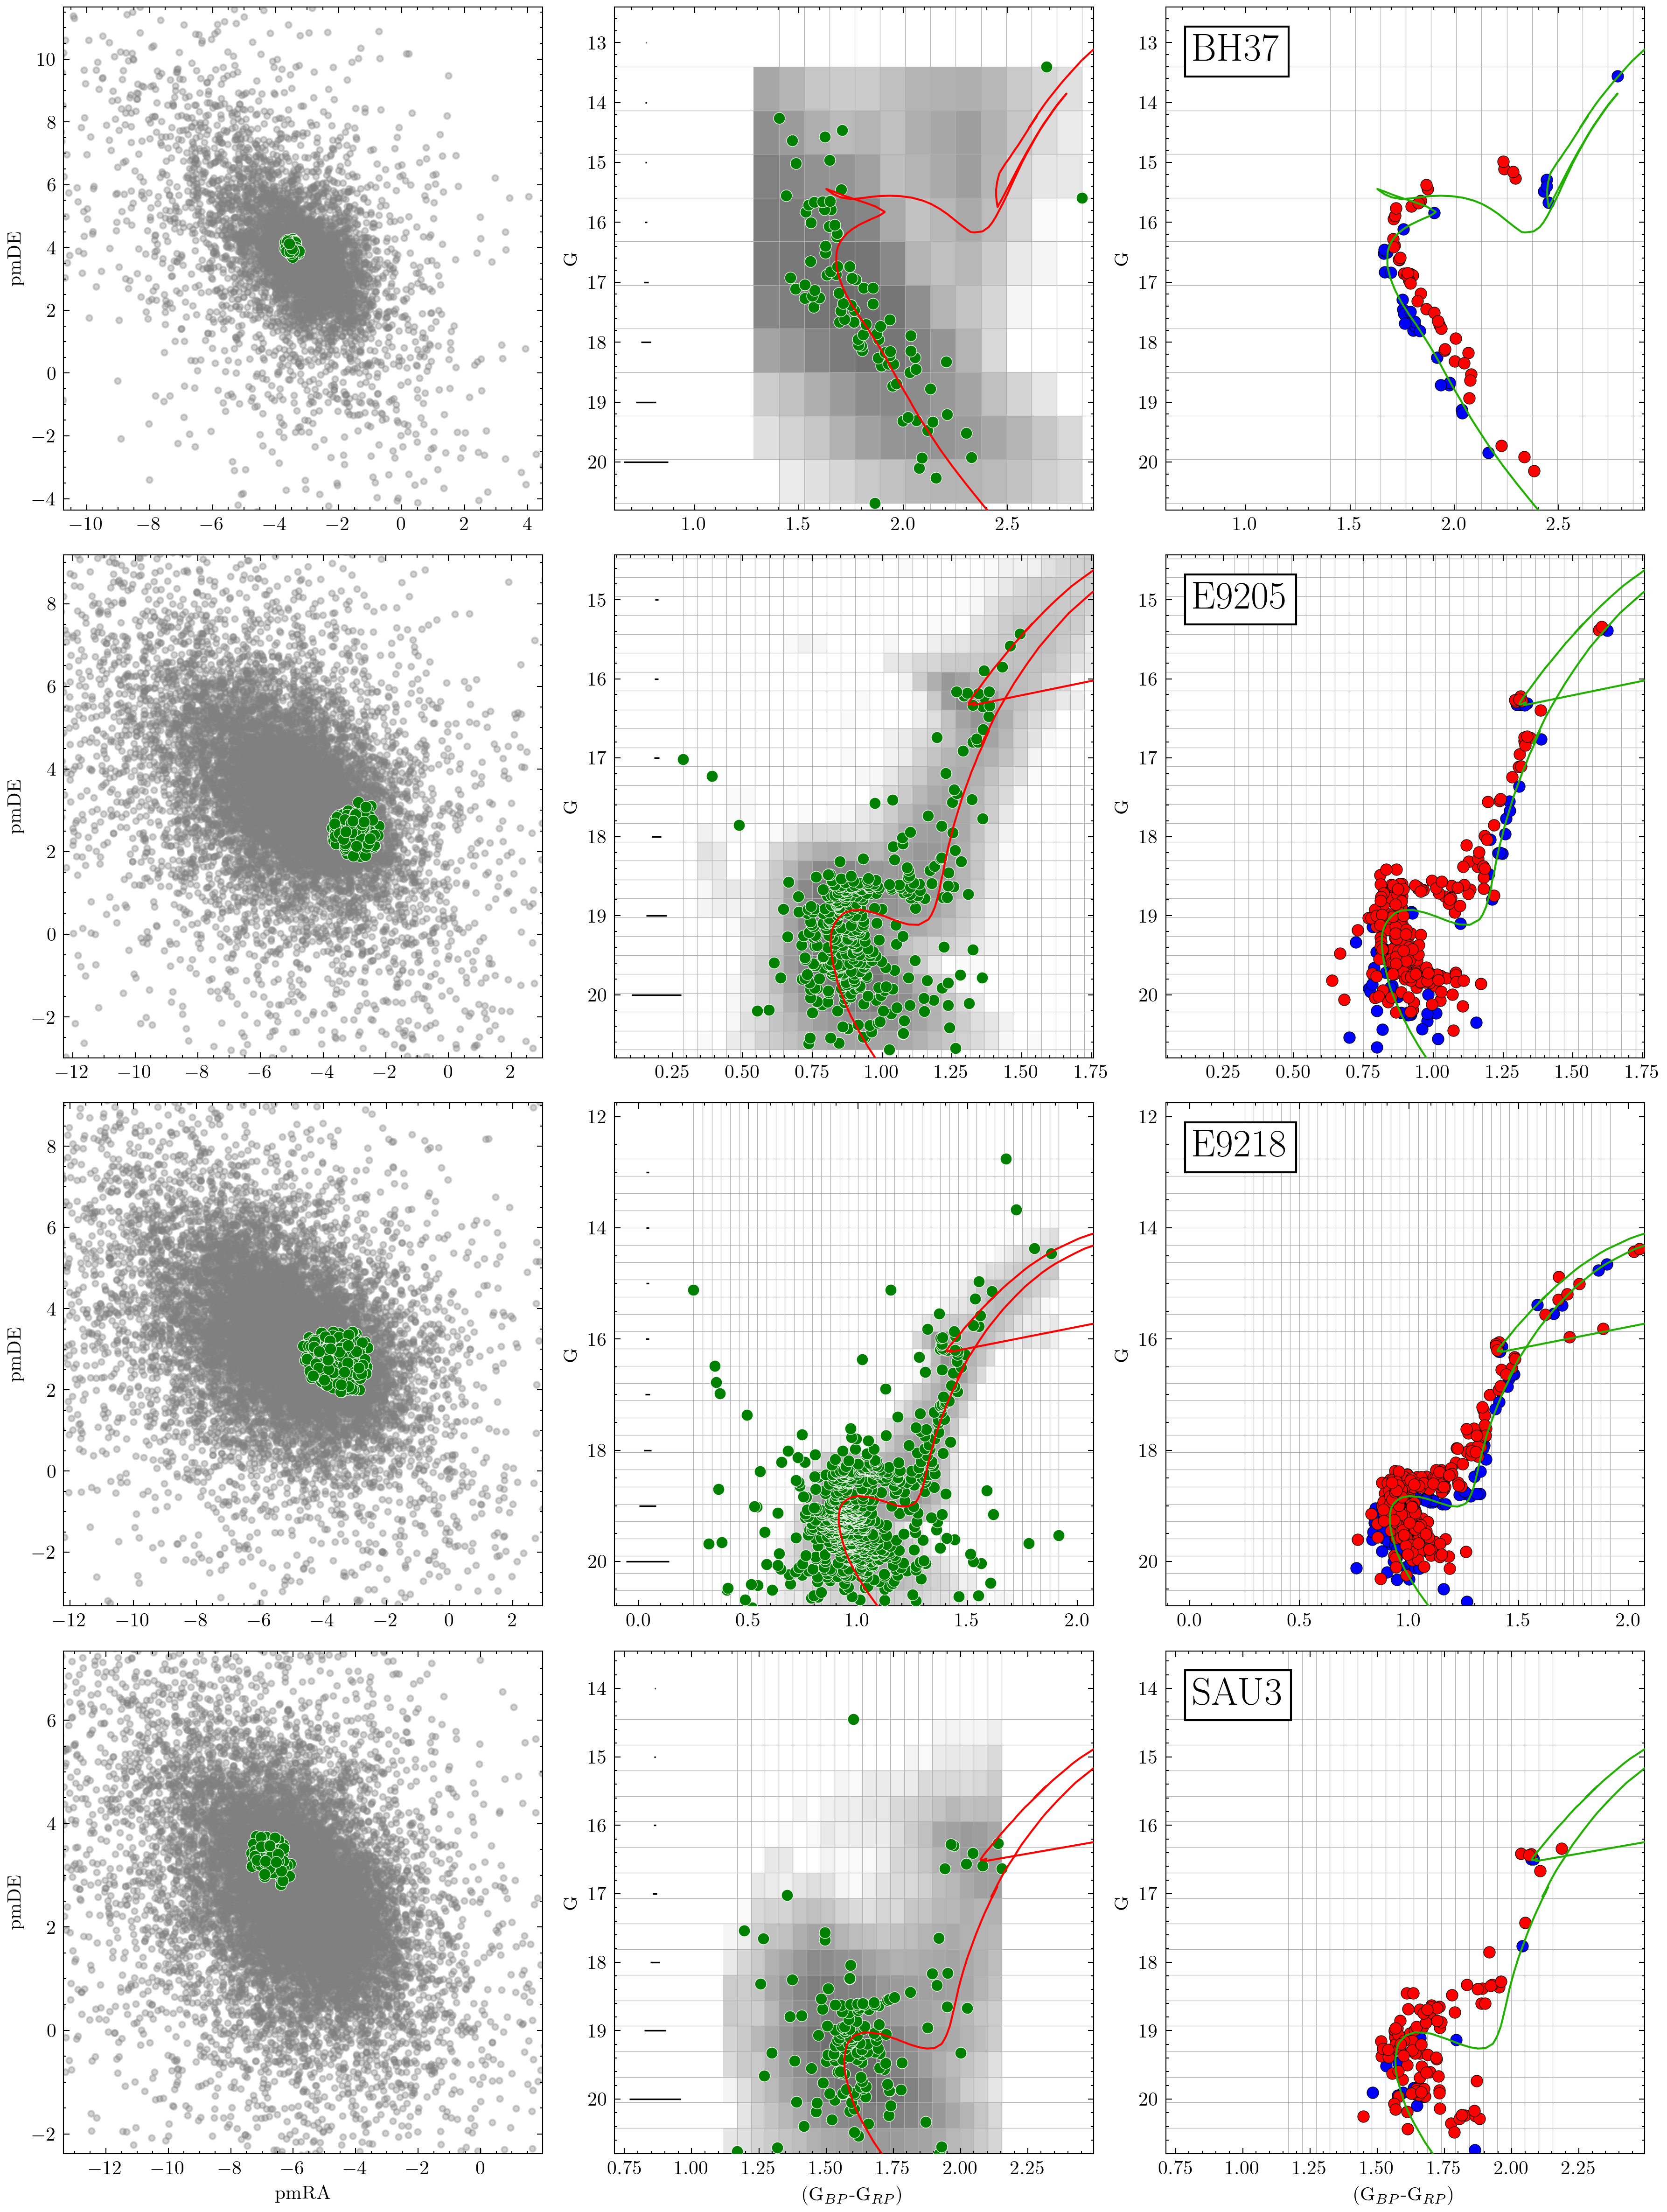
\includegraphics[height=.9\textheight]{figs/12_fpars.png}}
  \centering
  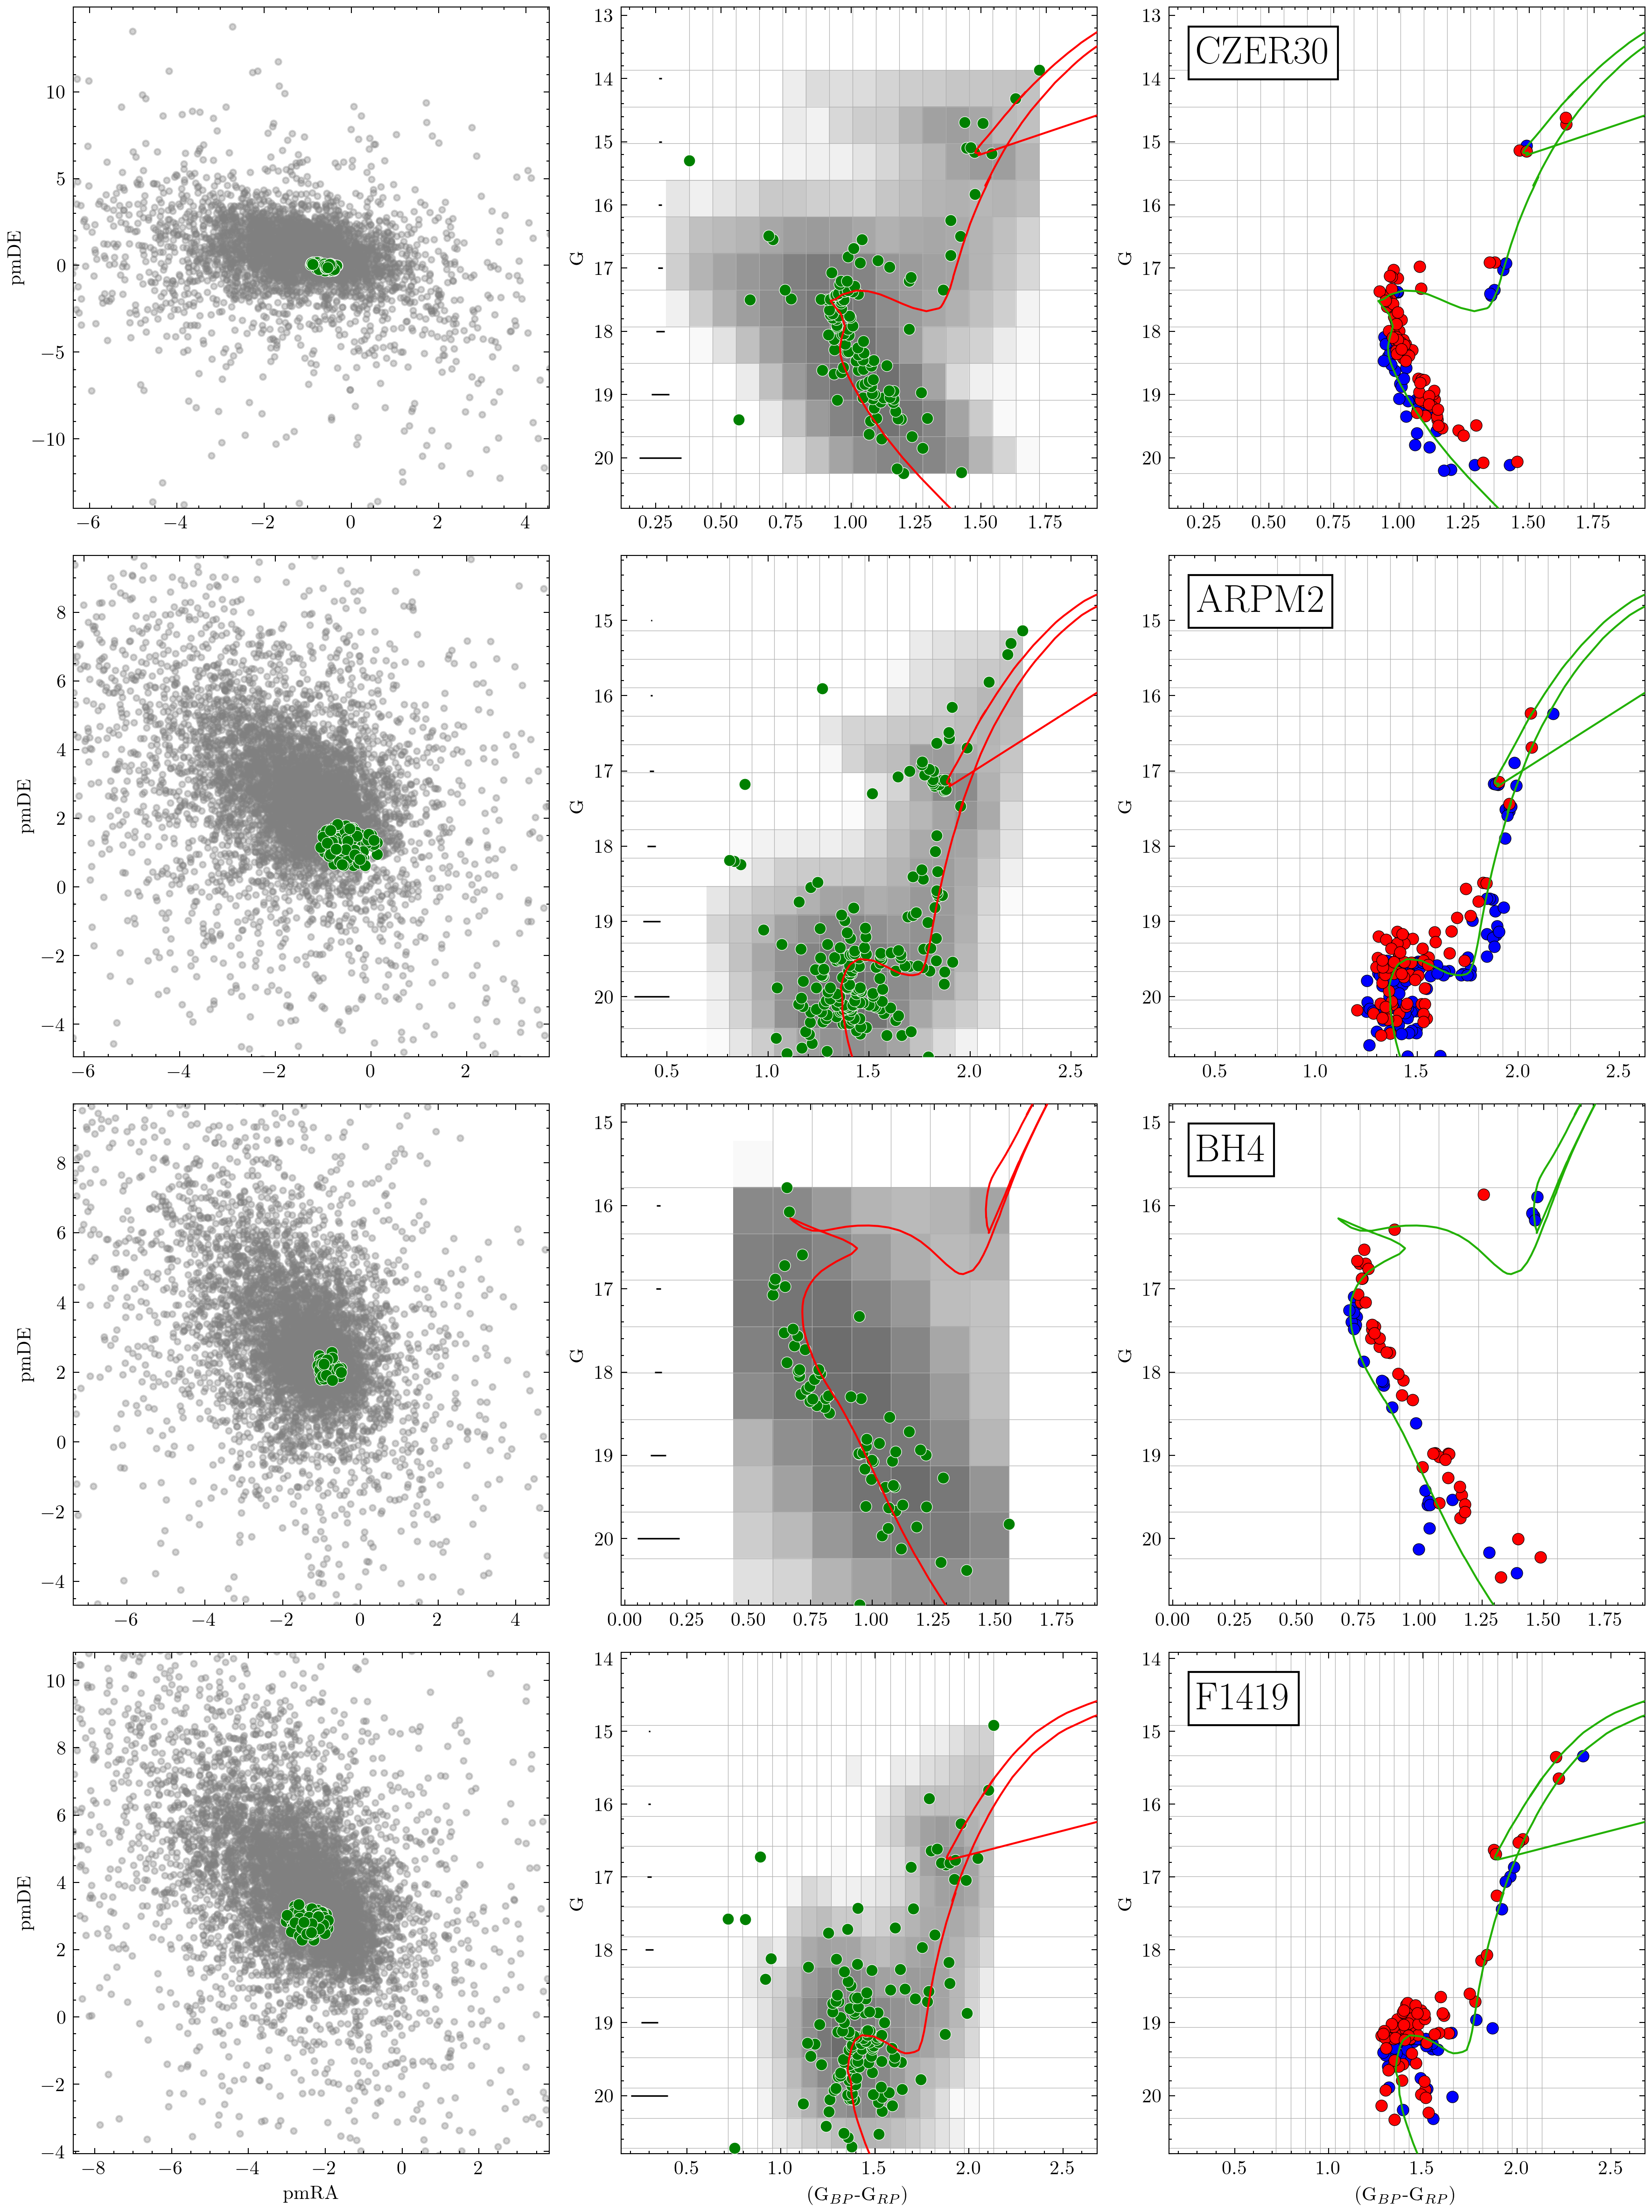
\includegraphics[height=.95\textheight]{figs/8_fpars.png}
  \caption{xxx}
  \label{fig:12fpars}
 \end{figure*}

 \begin{figure*}
  % \resizebox{\hsize}{!}{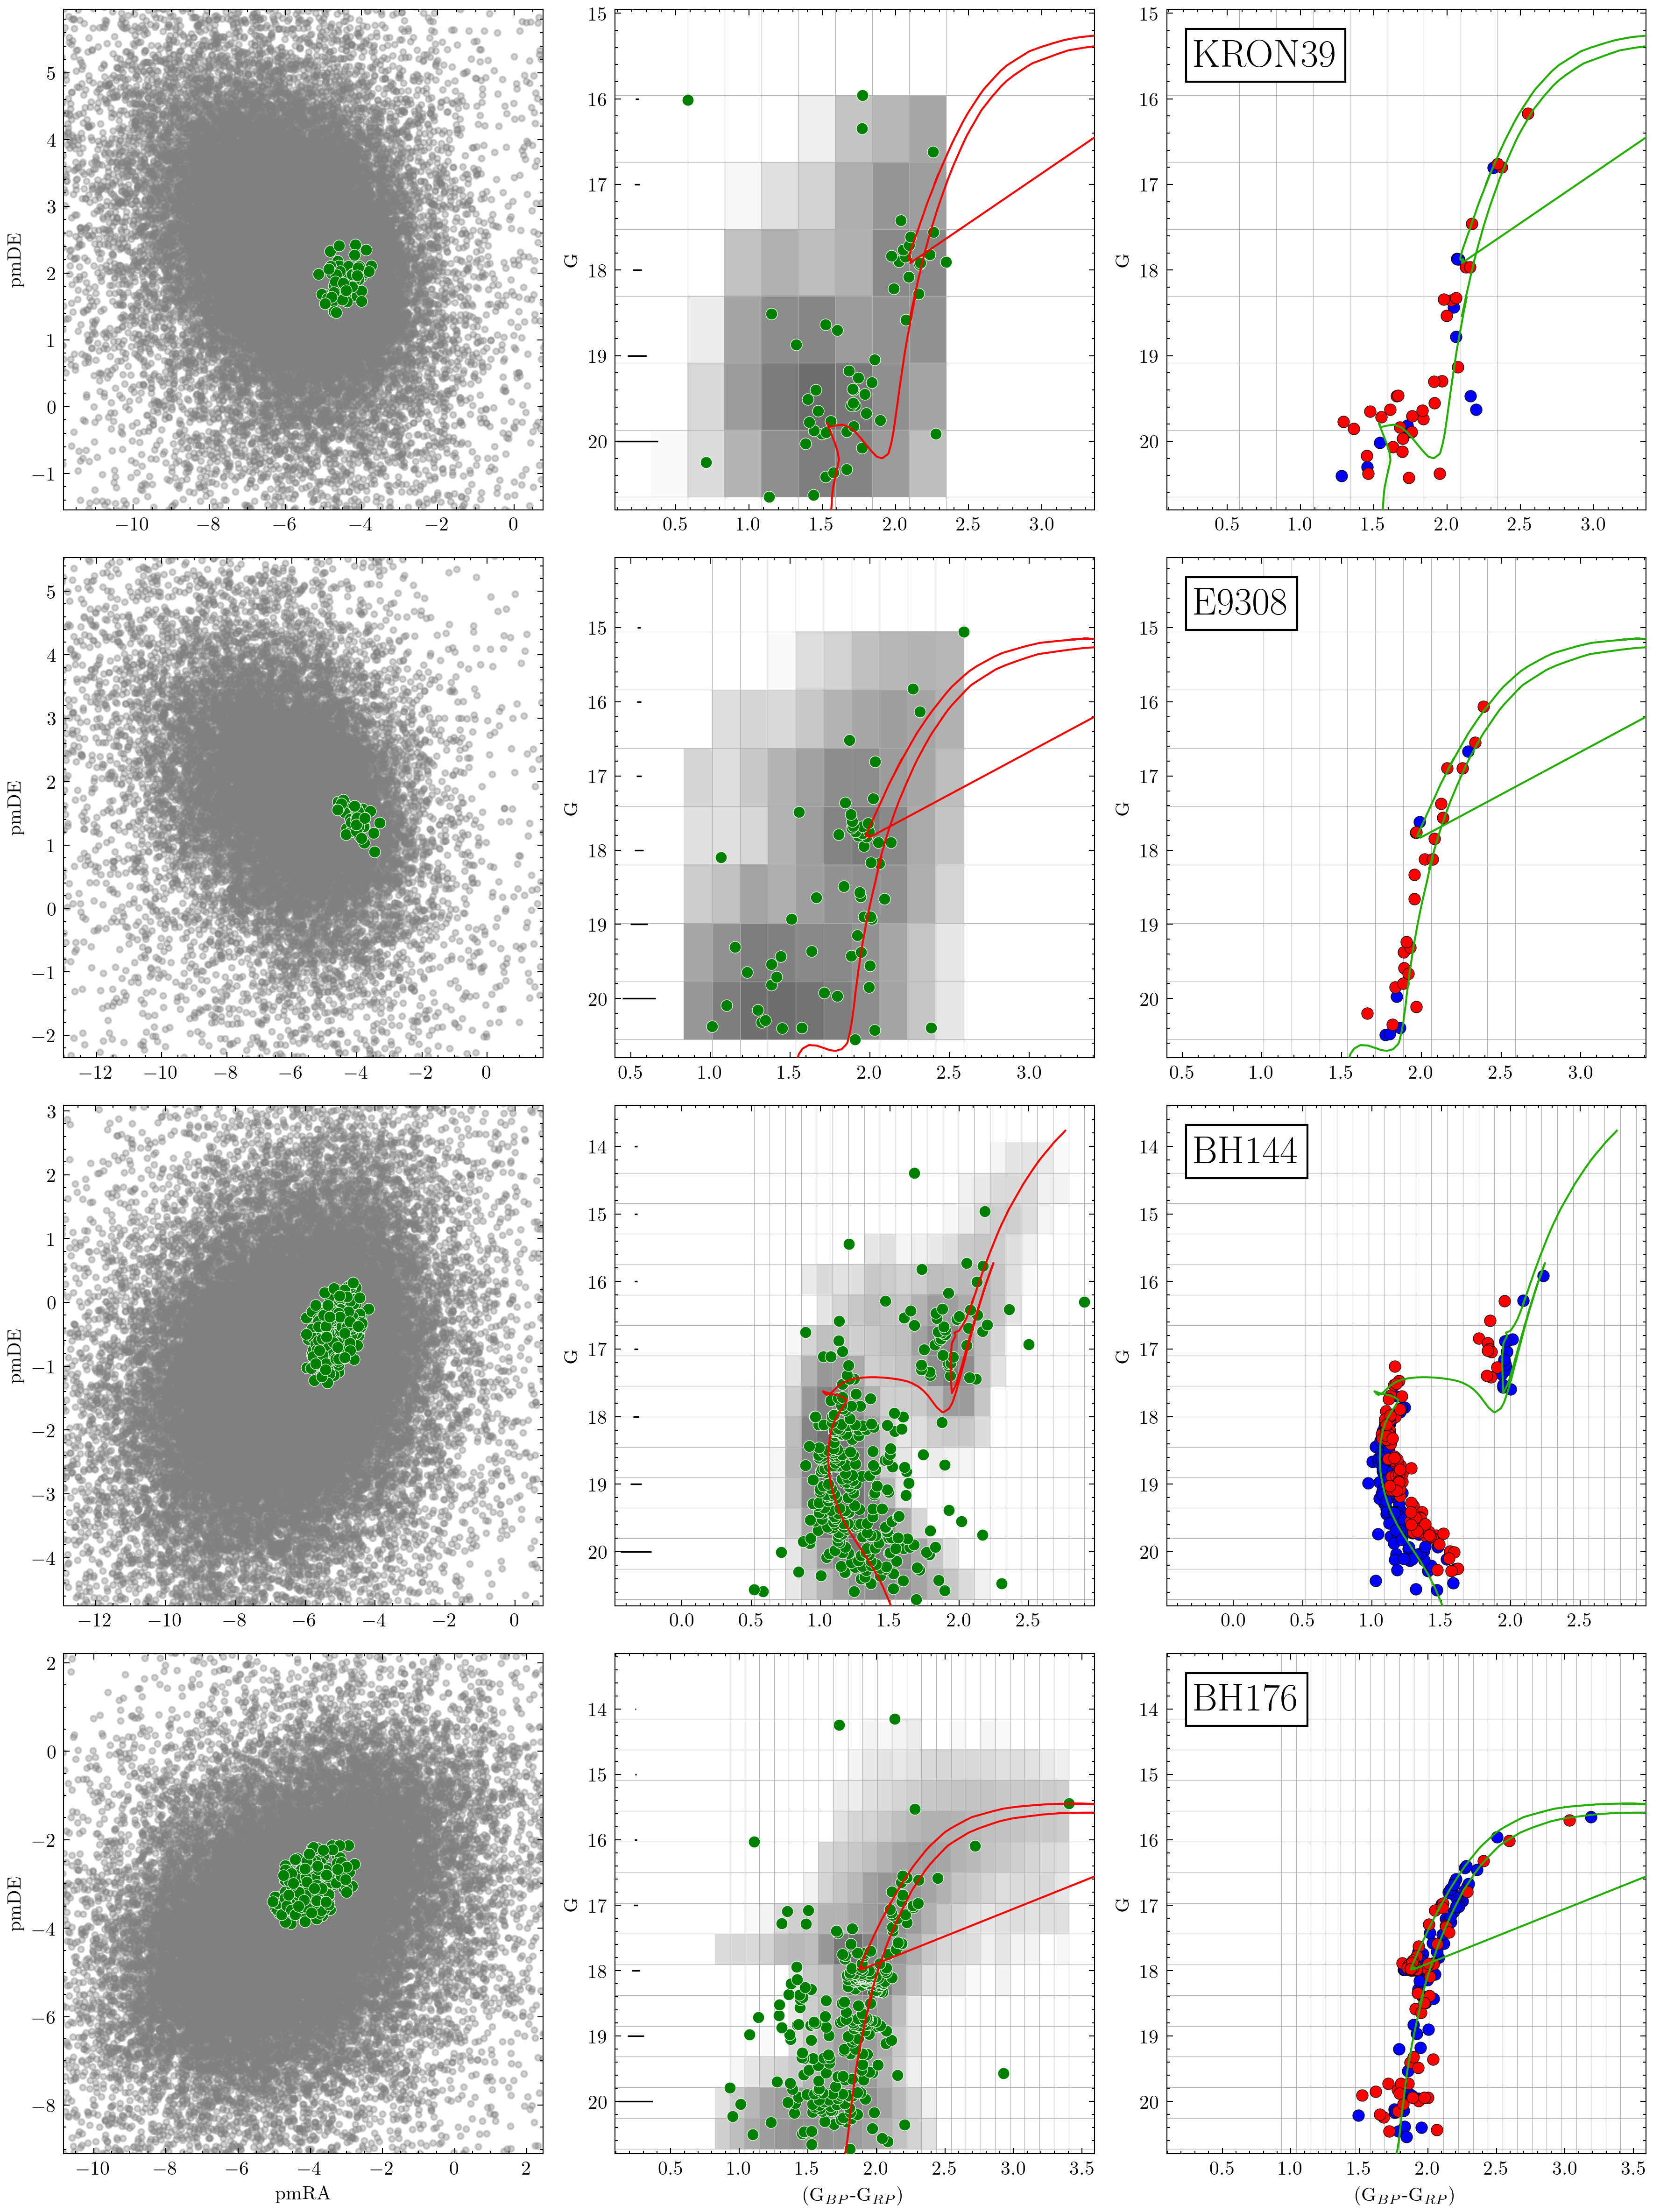
\includegraphics[height=.9\textheight]{figs/16_fpars.png}}
  \centering
  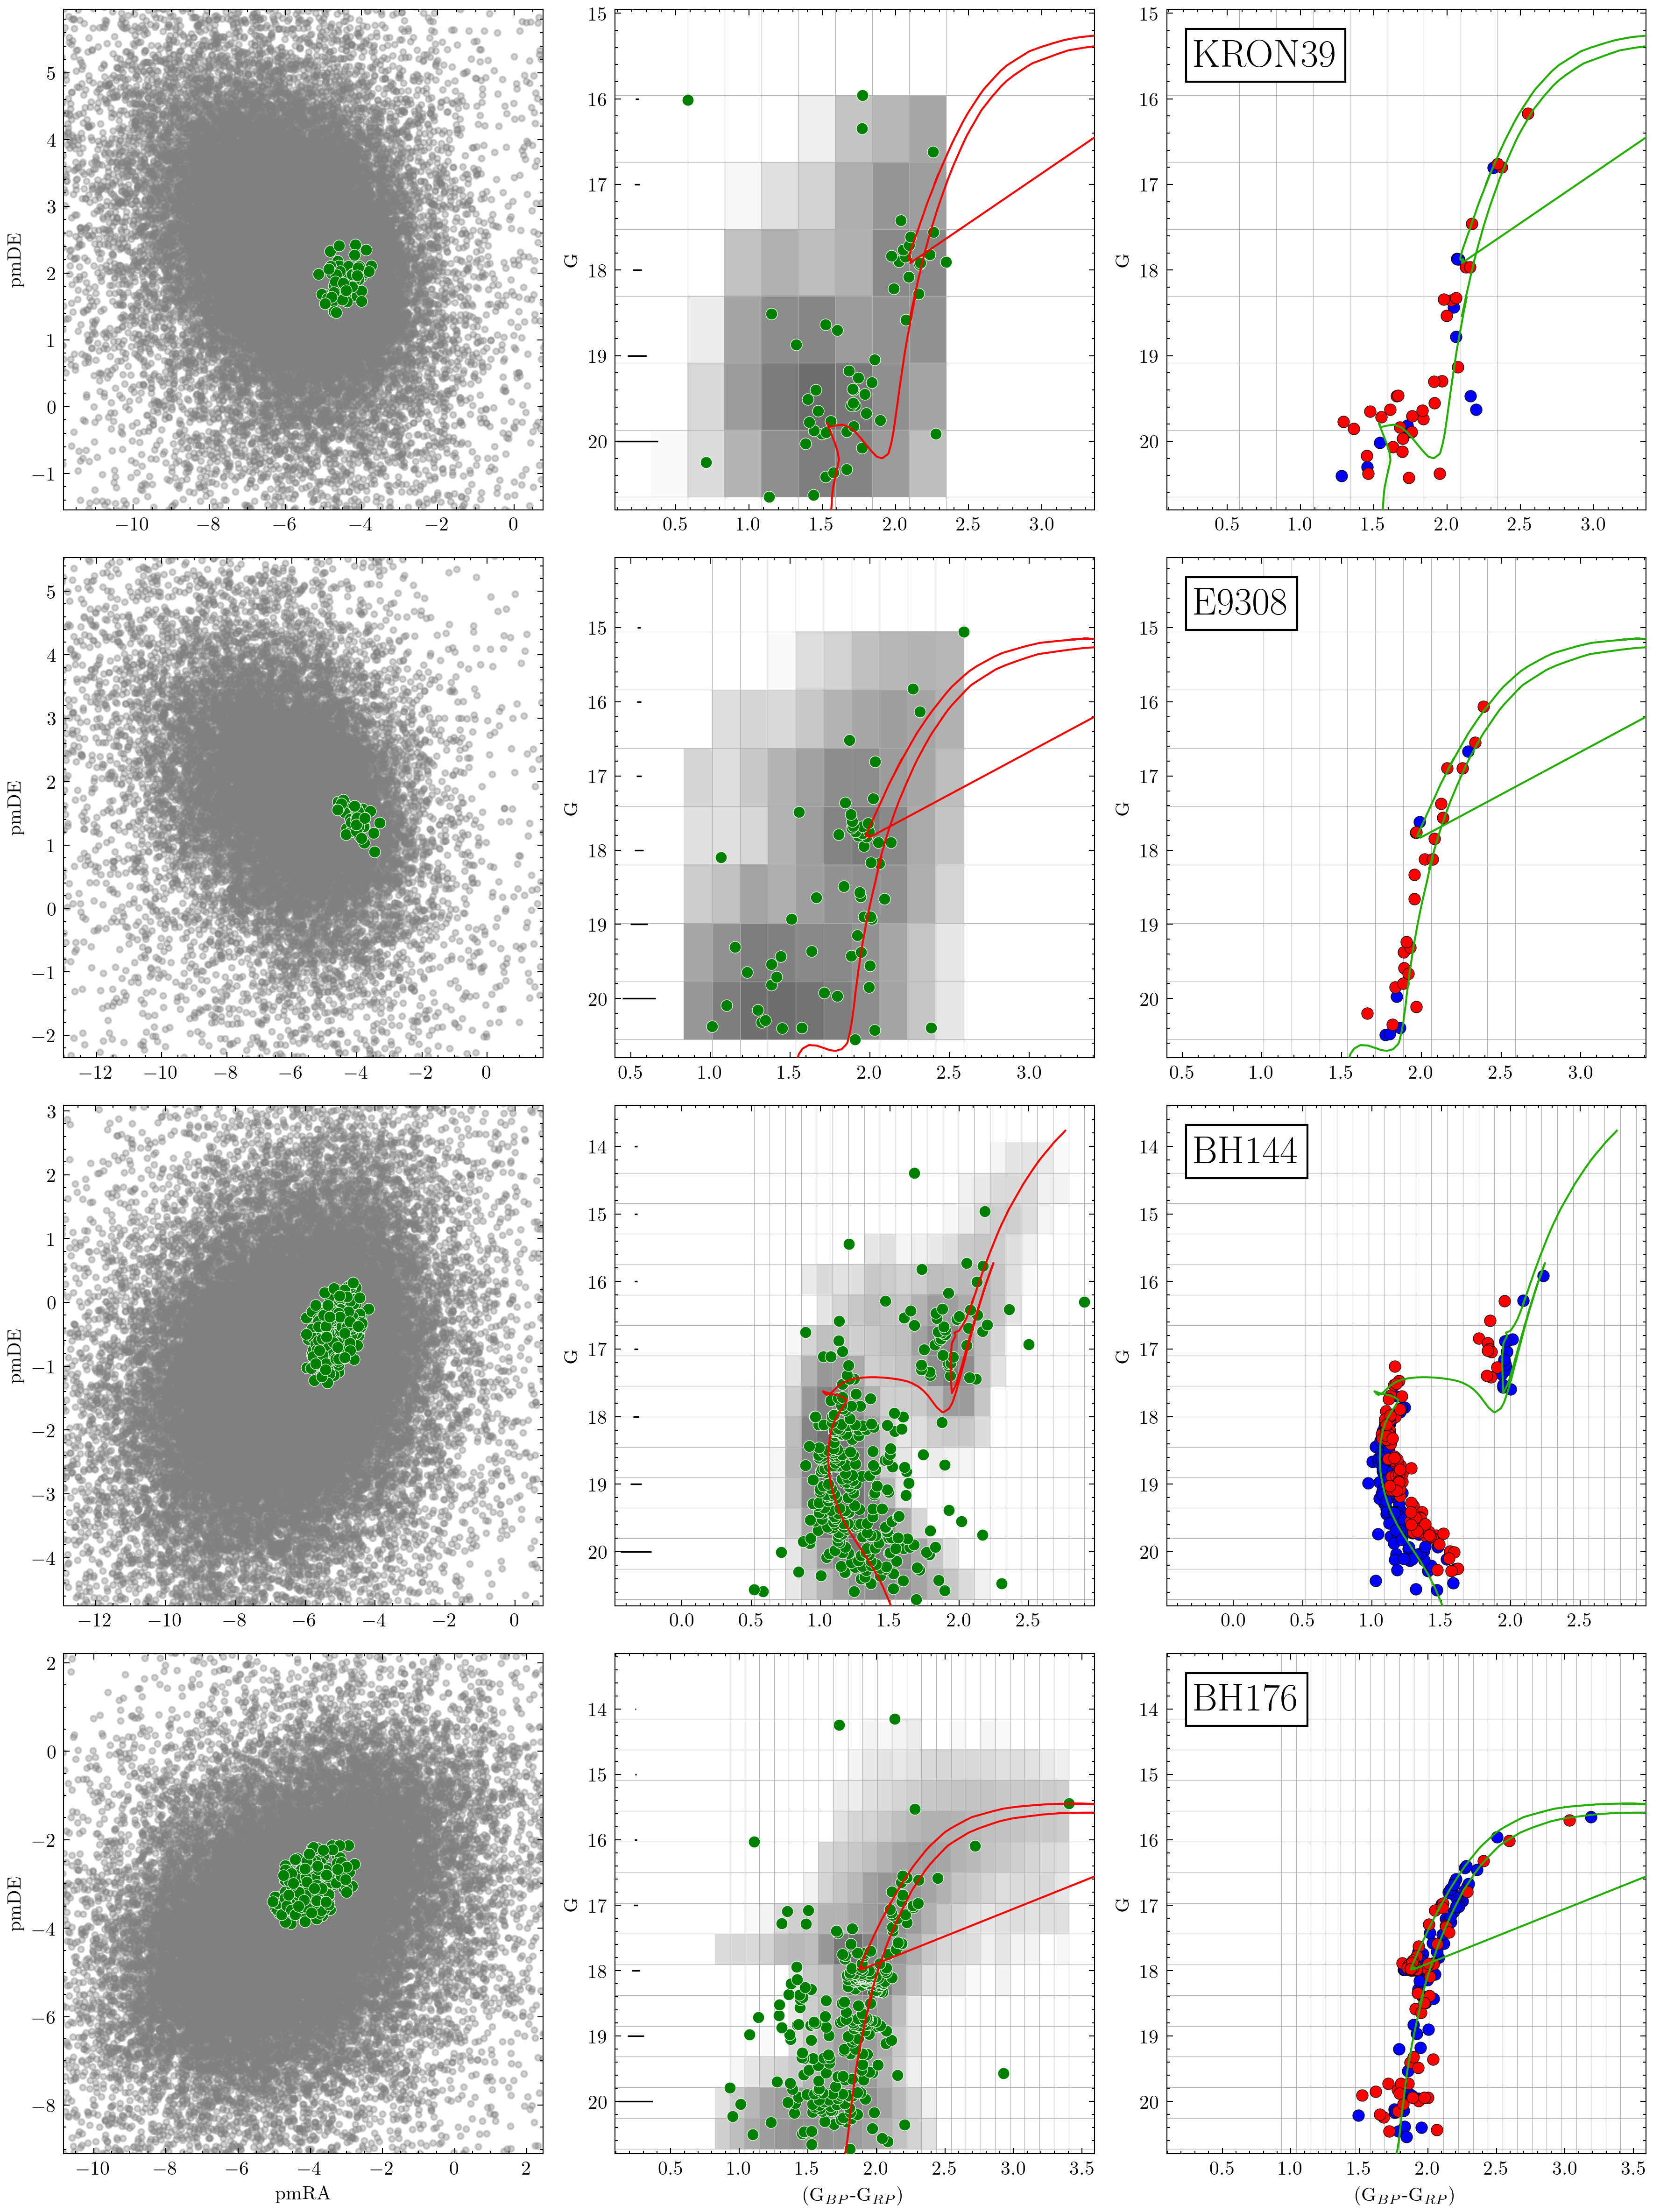
\includegraphics[height=.95\textheight]{figs/16_fpars.png}
  \caption{xxx}
  \label{fig:16fpars}
 \end{figure*}

 \begin{figure*}
  % \resizebox{\hsize}{!}{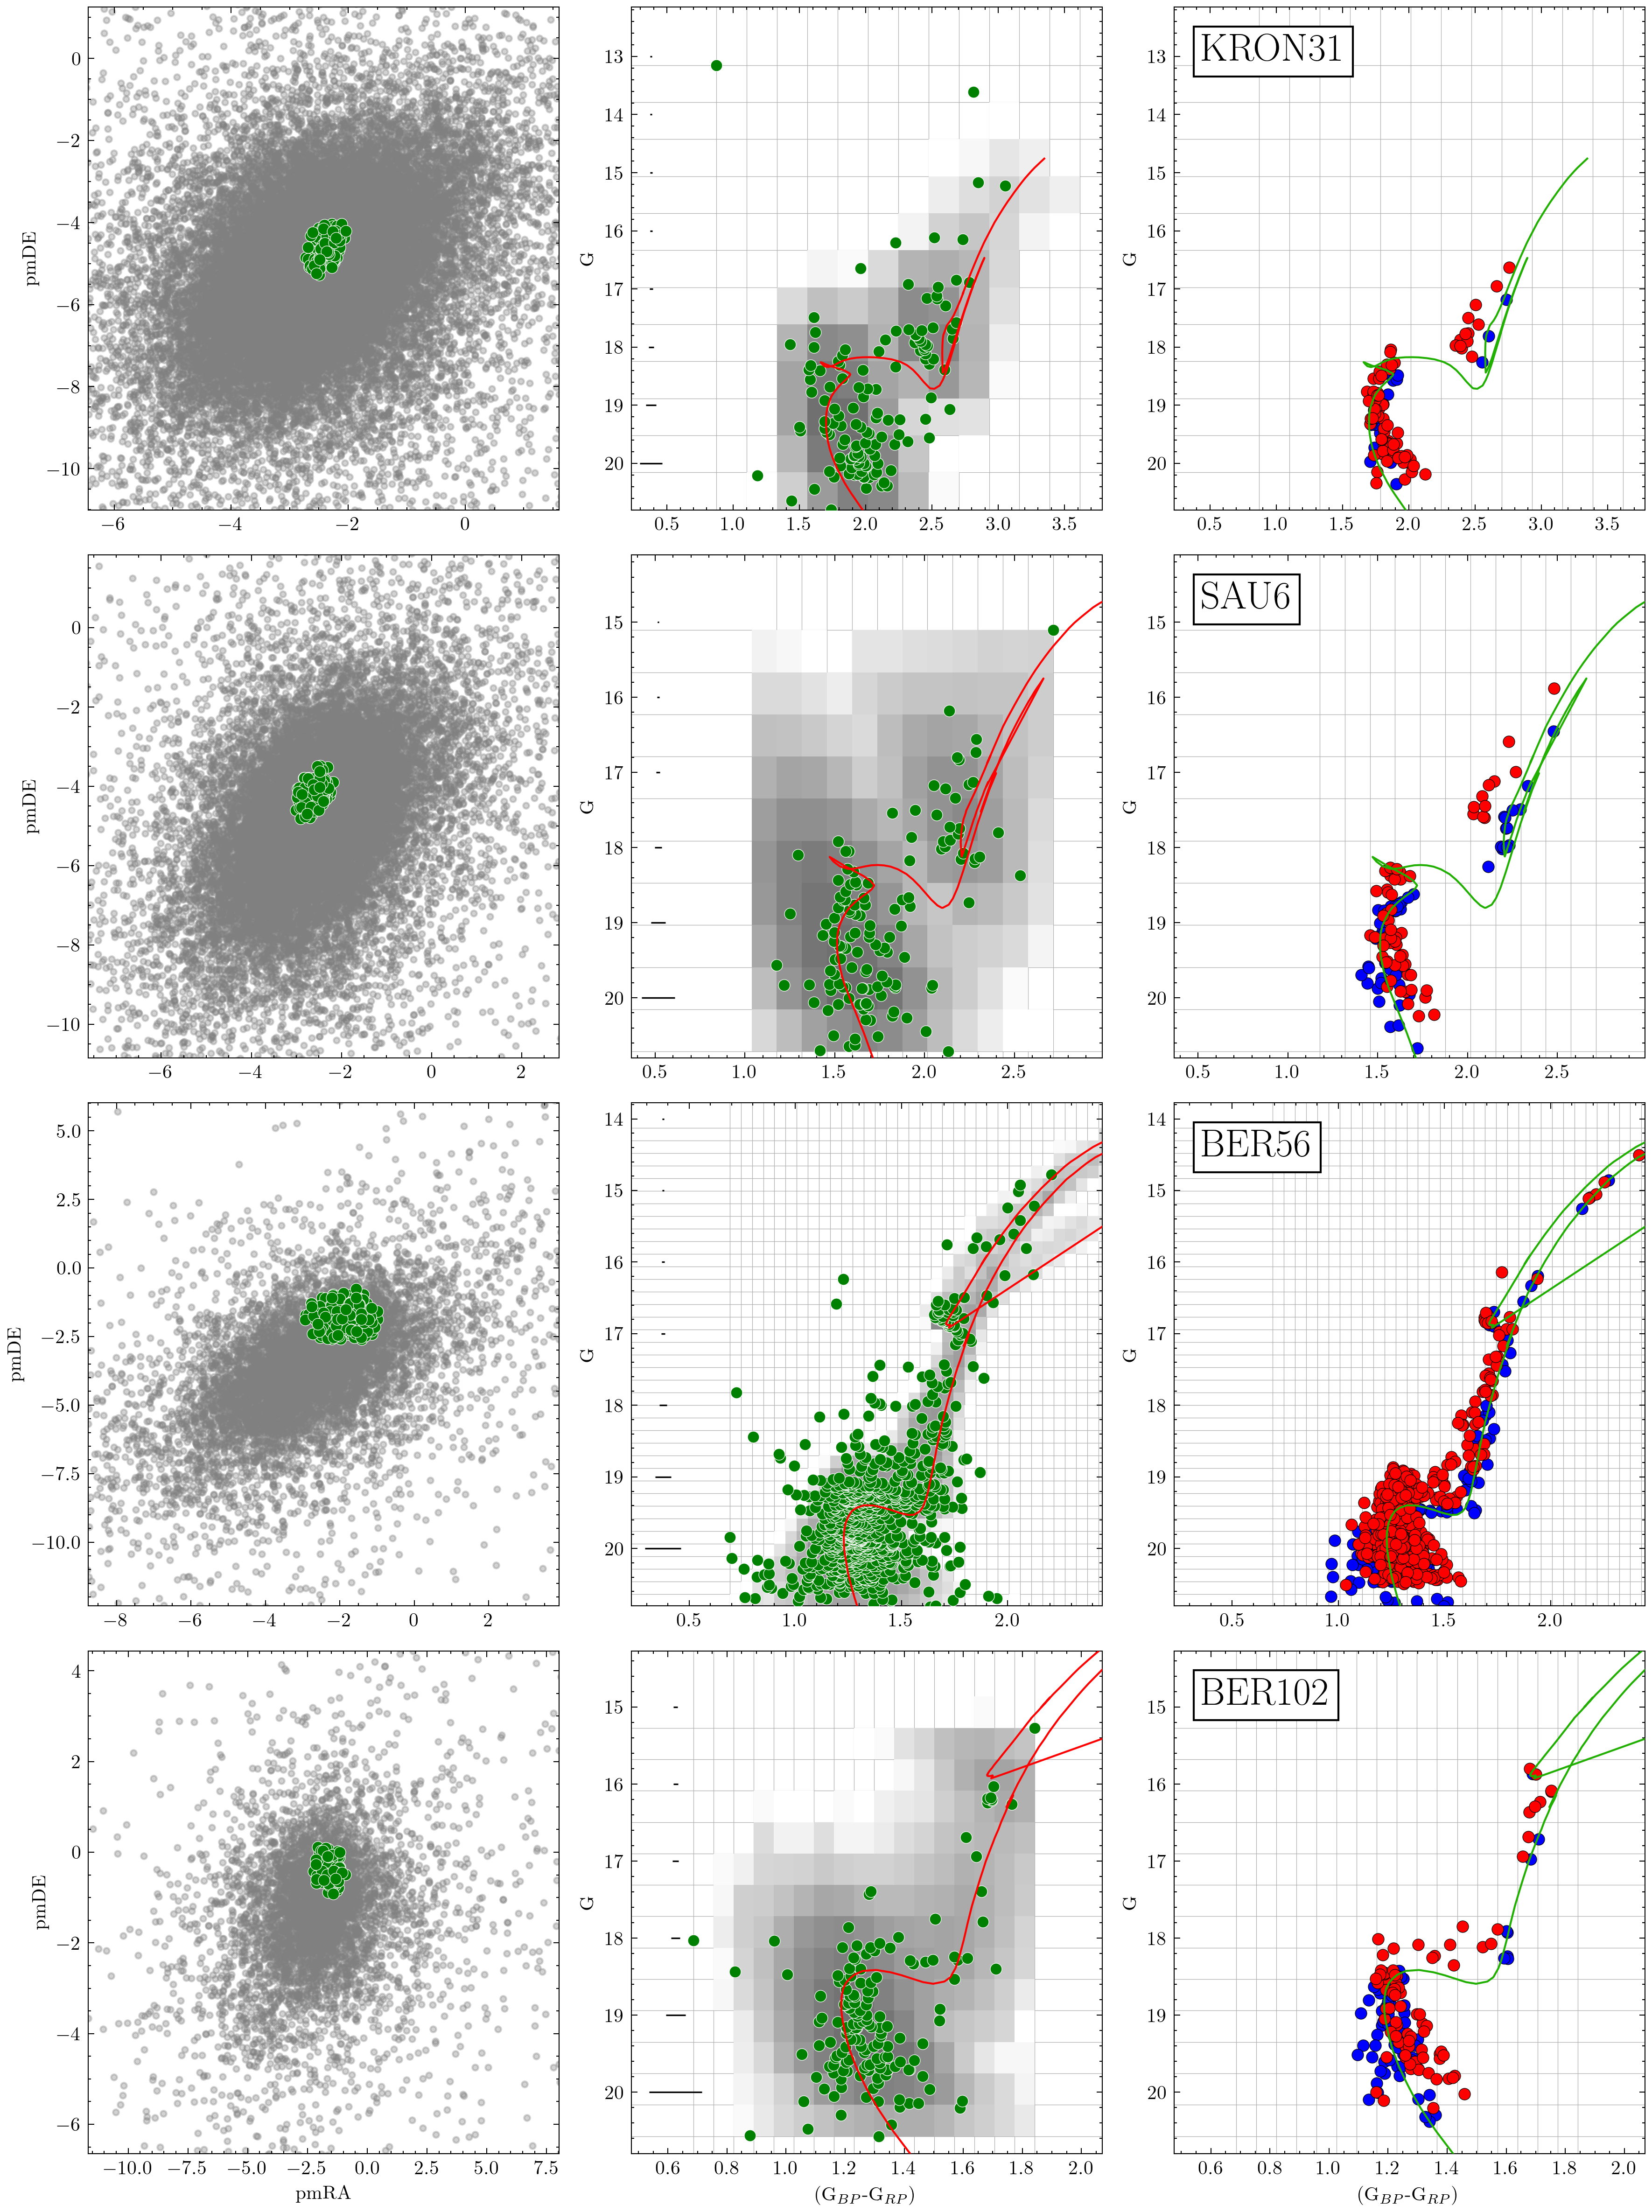
\includegraphics[height=.9\textheight]{figs/20_fpars.png}}
  \centering
  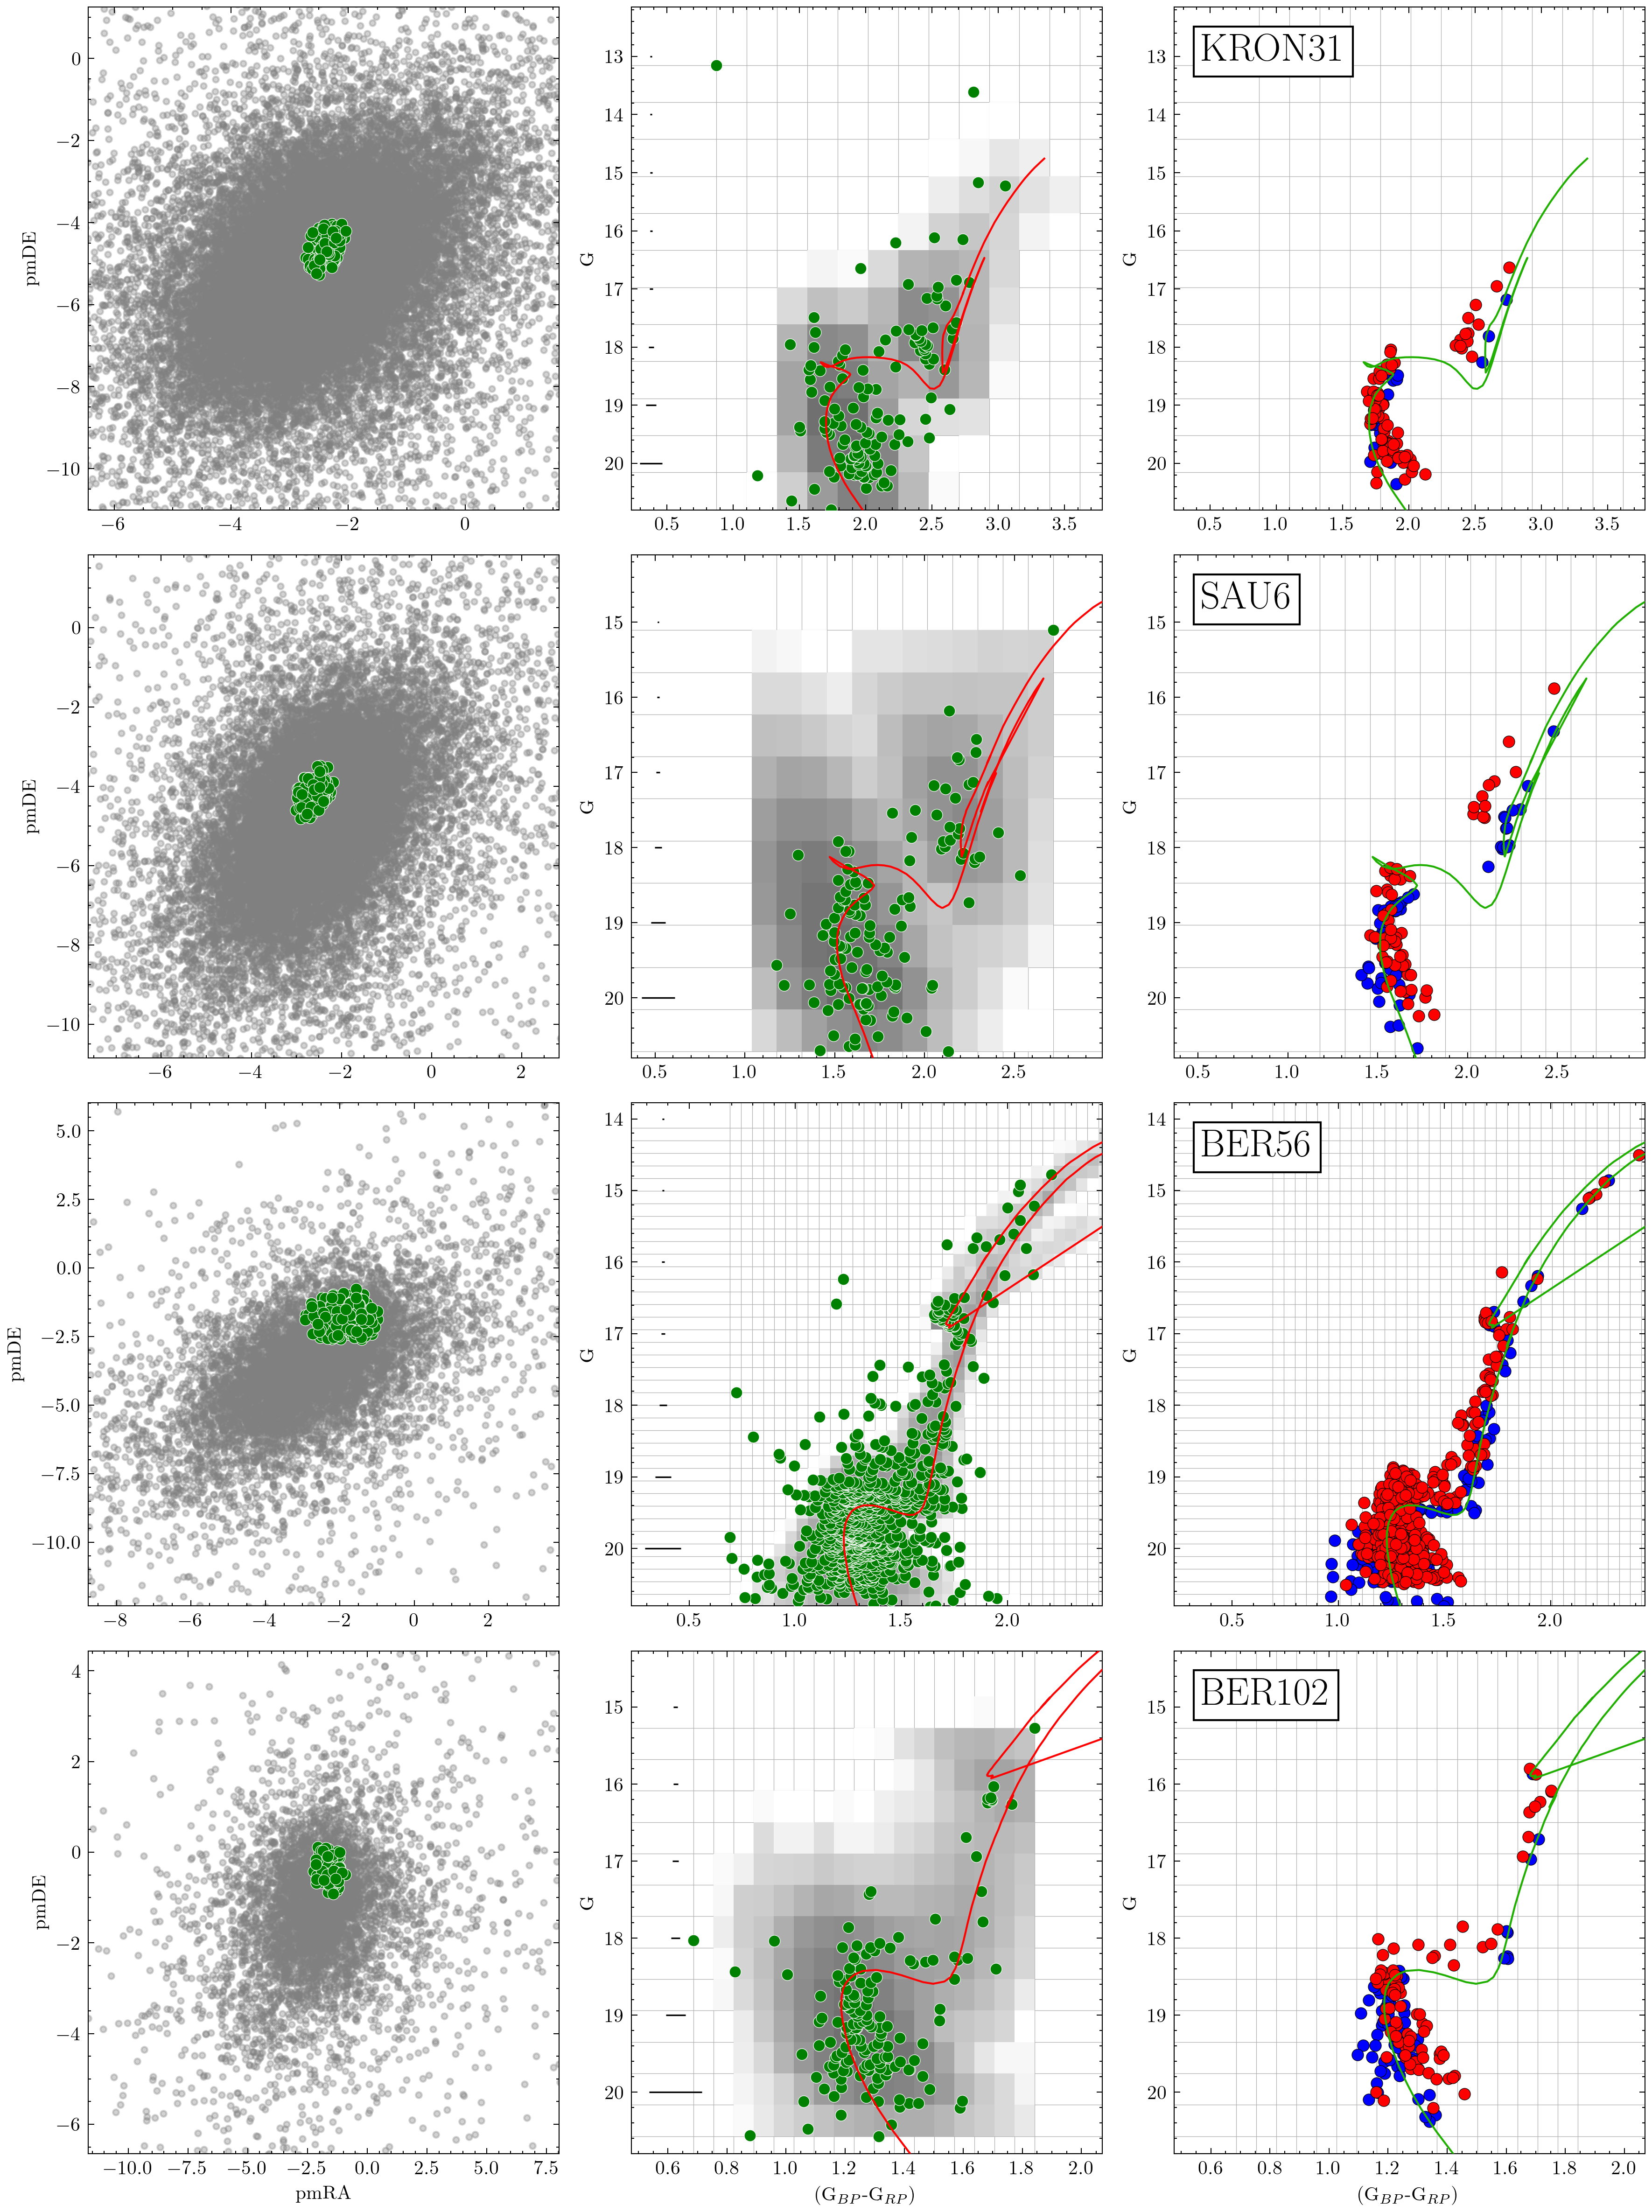
\includegraphics[height=.95\textheight]{figs/20_fpars.png}
  \caption{xxx}
  \label{fig:20fpars}
 \end{figure*}



\section{Galactocentric and dynamical parameters}
\label{app:galac_dynam}

  \begin{table*}
   \caption{[1]: \cite{Tarricq_2021}, [2]: \cite{Dias_2002}, [3]:
   \cite{Soubiran_2018}, [4]: \cite{Dias_2007}, [5]: \cite{Frinchaboy_2006}}
   \label{tab:velocities}
   \centering
   \renewcommand{\arraystretch}{1.3}
   \begin{tabular}{lccccccccc}
    \hline \hline
    $Cluster$ & $Dist$ & $R_{CG}$ & $X$ & $Y$ & $Z$ & $\mu_{\alpha}$ & $\mu_{\delta}$ & $RV$\\
     & [kpc] & [kpc] & [kpc] & [kpc] & [kpc] & [mas/yr] & [mas/yr] & [km/s]\\
    \hline
    BER73 & $4.89 \pm 0.02$ & 12.41 & -12.06 & -2.79 & -0.77 & $0.23\pm 0.17$ & $1.06 \pm 0.20$ & 112.41 [1]\\
    BER25 & $7.20 \pm 0.03$& 14.03 & -12.99 & -5.15 & -1.18 & $-0.13 \pm 0.14$ & $0.87 \pm 0.18$ & 108.07 [1]\\
    BER75 & $7.95 \pm 0.04$ & 14.25 & -12.68 & -6.33 & -1.51 & $-0.22 \pm 0.12$ & $1.14 \pm 0.17$ & 122.41 [1]\\
    BER26 & $4.75 \pm 0.02$ & 12.52 & -12.32 & -2.20 & 0.23 & $0.16 \pm 0.28$ & $0.38 \pm 0.26$ & 68.00 [2]\\
    BER29 & $14.16 \pm 0.07$ & 21.98 & -21.46 & -4.32 & 2.02 & $0.15 \pm 0.28$ & $-1.05 \pm 0.27$ & 25.72 [1] \\
    TOMB2 & $8.89 \pm 0.04$ & 15.22 & -13.46 & -7.04 & -1.03 & $-0.49 \pm 0.23$ & $1.39 \pm 0.28$ & 122.47 [1]\\
    BER76 & $5.49 \pm 0.03$ & 12.61 & -12.00 & -3.89 & -0.16 & $-0.60 \pm 0.18$ & $1.41 \pm 0.14$ & 73.02 [1]\\
    F1212 & $10.15 \pm 0.05$ & 16.74 & -14.99 & -7.45 & -0.47 & $-0.34 \pm 0.15$ & $0.52 \pm 0.20$ & 71.82 [1]\\
    SAU1 & $12.50 \pm 0.06$ & 19.69 & -18.31 & -7.05 & 1.65 & $-0.29 \pm 0.29$ & $-0.25 \pm 0.27$ & 98.00 [2]\\
    CZER30 & $6.57 \pm 0.03$ & 13.52 & -12.64 & -4.75 & 0.51 & $-0.62 \pm 0.12$ -& $0.07 \pm 0.11$ & 82.07 [1]\\
    ARMP2 & $10.97 \pm 0.05$ & 15.89 & -12.19 & -10.13 & -1.09 & $-0.49 \pm 0.23$ & $1.25 \pm 0.26$ & 58.25 [1]\\
    BH4 & $7.89 \pm 0.04$ & 13.10 & -10.80 & -7.35 & -0.95 & $-0.82 \pm 0.14$ & $2.12 \pm 0.16$ & -- \\
    F1419 & $9.33 \pm 0.04$ & 12.99 & -9.09 & -9.22 & -1.05 & $-2.48 \pm 0.24$ & $2.85 \pm 0.21$ & --\\
    BH37 & $2.78 \pm 0.01$ & 8.92 & -8.49 & -2.75 & -0.06 & $-3.50 \pm 0.09$ & $3.99 \pm 0.11$ & 51.90 [3]\\
    E9205 & $13.03 \pm 0.06$ & 13.31 & -4.53 & -12.40 & -1.69 & $-3.00 \pm 0.29$ & $2.48 \pm 0.23$ & 57.40 [1]\\
    E9218 & $11.15 \pm 0.05$ & 11.72 & -4.86 & -10.58 & -1.28 & $-3.59 \pm 0.36$ & $2.72 \pm 0.27$ &  --\\
    SAU3 & $6.61 \pm 0.03$ & 9.04 & -6.40 & -6.37 & 0.36 & $-6.70 \pm 0.24$ & $3.29 \pm 0.19$ & --\\
    KRON39 & $12.84 \pm 0.06$ & 12.70 & -3.83 & -12.10 & -0.43 & $-4.42 \pm 0.35$ & $1.89 \pm 0.23$ & --\\
    E9308 & $13.26 \pm 0.06$ & 12.50 & -2.85 & -12.13 & -0.93 & $-4.04 \pm 0.24$ & $1.38 \pm 0.17$ & 86.00 [2]\\
    BH144 & $9.55 \pm 0.04$ & 8.22 & -2.60 & -7.78 & -0.52 & $-5.14 \pm 0.33$ & $-0.47 \pm 0.32$ & 40.00 [4]\\
    BH176 & $19.78 \pm 0.09$ & 13.57 & 8.69 & -10.32 & 1.47 & $-3.97 \pm 0.45$ & $-3.07 \pm 0.36$ & 11.20 [5]\\
    KRON31 & $8.27 \pm 0.04$ & 8.40 & -4.20 & 7.27 & 0.28 & $-2.36 \pm 0.15$ & $-4.62 \pm 0.29$ & --\\
    SAU6 & $9.34 \pm 0.04$ & 9.82 & -4.63 & 8.65 & 0.47 & $-2.60 \pm 0.18$ & $-4.15 \pm 0.29$ & --\\
    BER56 & $11.00 \pm 0.05$ & 13.21 & -7.36 & 10.93 & -0.98 & $-1.92 \pm 0.32$ & $-1.81 \pm 0.32$ & -54.95 [1]\\
    BER102 & $7.68 \pm 0.04$ & 13.18 & -11.12 & 7.05 & -0.62 & $-1.56 \pm 0.25$ & $-0.36 \pm 0.21$ & --\\
    \hline
    \end{tabular}
  \end{table*}

\end{appendix}

\end{document}


